\documentclass[ngerman]{article}

\usepackage{fancyhdr}
\usepackage{hyperref}
\usepackage{nameref}
\usepackage{babel}
\usepackage{graphicx}
\usepackage{csquotes}
\usepackage{enumitem}
\usepackage{tabularx}
\usepackage{graphicx}
\usepackage{subcaption}
\usepackage{booktabs}

\MakeOuterQuote{"}
% * = Hartes Kriterium
% 
% „Einfache“ Programmierung
% GUI Designer für die schnelle Oberflächenprogrammierung
% Zukunftssicher
% Umfangsreiche Bibliotheksfunktionen vom Framework/Sprache
% * Verfügbarkeit auf Desktop und Mobilen Geräten(Web-Entwicklung?)
% * Keine App-Store-Abhängigkeit, da kein Internet in der Regel auf den Endgeräten verfügbar
% Sprache/Framework populär? Unten 20 beliebtesten Sprachen von 2019/2020
% Zukunftssicherheit: Verlauf der letzten 10 Jahre betrachten
% * „Einfache“ Wartung + Pflege
\setenumerate{itemsep=-.5em}
\newcounter{mylabelcounter}

\makeatletter
\newcommand{\labelText}[2]{%
#1\refstepcounter{mylabelcounter}%
\immediate\write\@auxout{%
  \string\newlabel{#2}{{1}{\thepage}{{\unexpanded{#1}}}{mylabelcounter.\number\value{mylabelcounter}}{}}%
}%
}
\makeatother
\begin{document}
    \sloppy
    \pagestyle{empty}
    %%%%%%%%%%%%%%%%%%%%%%%%%% Deckblatt %%%%%%%%%%%%%%%%%%%%%%%%%%
    \begin{figure}
        \begin{center}
            {\huge\textbf{Philipps-Universität Marburg}}\\
            \vspace{.2cm}
            {\small \textbf{Fachbereich 12 - Mathematik und Informatik}}\\\vspace{.5cm}
            \vspace{.2cm}
            %
\includegraphics[width=1\textwidth]{Uni Logo.png}\vspace{1cm}
            %\vspace{.5cm}
            {\huge\textbf{Siemens Marburg}}\\
            \vspace{1.5cm}
            {\LARGE\textbf{Analyse und Vergleich verschiedener Softwaretechnologien zur Entwicklung einer neuen Technologieplattform für die Siemens Applikation: "Opcenter Execution Pharma"}}\\
            \vspace{.5cm}
            \textbf{von Jonas Borgerding}
        \end{center}
    \end{figure}
    \clearpage
    \noindent
    %%%%%%%%%%%%%%%%%%%%%%%%%% Sperrvermerk %%%%%%%%%%%%%%%%%%%%%%%%%%
    \hspace*{\fill}{\Huge\textbf{Sperrvermerk}}\hspace*{\fill}\\\\\\
    \begin{center}
        Die vorgelegte Bachelorarbeit mit dem Titel „Analyse und Vergleich verschiedener Softwaretechnologien zur Entwicklung einer neuen Technologieplattform für die Siemens Applikation: "Opcenter Execution Pharma"“ beinhaltet vertrauliche Informationen und Daten des Unternehmens Siemens.
    \end{center}
    \vspace{4mm}
    \begin{center}
        Diese Bachelorarbeit darf nur vom Erst- und Zweitgutachter sowie berechtigten Mitgliedern des Prüfungsausschusses eingesehen werden. Eine Vervielfältigung und Veröffentlichung der Bachelorarbeit ist auch auszugsweise nicht erlaubt.
    \end{center}
    \vspace{4mm}
    \begin{center}
        Dritten darf diese Arbeit nur mit der ausdrücklichen Genehmigung des Verfassers und Unternehmens zugänglich gemacht werden.
    \end{center}
    \newpage
    %%%%%%%%%%%%%%%%%%%%%%%%%% Erklärung %%%%%%%%%%%%%%%%%%%%%%%%%%
    \textbf{Erklärung}\\
    Ich, Jonas Borgerding (Informatikstudent an der Philipps-Universität Marburg, Matrikelnummer 3111336), versichere an Eides statt, dass ich die vorliegende Bachelorarbeit selbstständig verfasst und keine anderen als die angegebenen Quellen und Hilfsmittel verwendet habe. Die hier vorliegende Bachelorarbeit wurde weder in ihrer jetzigen noch in einer ähnlichen Form einer Prüfungskommission vorgelegt.\\\\\\
    Stadtallendorf, \today\\\\
    Jonas Borgerding\newpage
    %\hspace*{\fill}\textbf{Zusammenfassung}\hspace*{\fill}\\
    %Das bestehende System "Opcenter Execution Pharma" wurde in VB6 entwickelt. Da VB6 seit 2005 keinen Support mehr erhält und es in der Pharmaindustrie, wegen einhaltung von bestimmten Qualitätsanforderungen, sehr lange dauert ein System neu zu Implementieren, ist es dringend notwendig auf eine neue, moderne Technologieplattform umzusteigen, welche möglichst Zukunftssicher ist, da ein Umstieg auf eine neue Technologieplattform nicht so einfach ist. Diese Bachelorthesis beschäftigt sich damit herauszufinden, welche neuen Technologien extistieren und welche Technologie für die Neuentwicklung des Projekt "Opcenter Execution Pharma", unter Beachtung mehrerer Aspekte, am besten geeignet ist.\\\indent Als erstes wird untersucht, auf welche Technologieplattform entwickelt werden sollte. Der nächste Schritt ist die Auswahl von geeigneten Programmiersprachen für die ausgewählte Plattform. Anschließend werden für die gefilterten Programmiersprachen maximal 3 Frameworks herausgesucht. Zum Schluss werden in den letzten wenigen Frameworks jeweils das selbe Modul entwickelt.\newpage
    \tableofcontents\newpage
    \pagestyle{fancy}
    \renewcommand{\sectionmark}[1]{\markright{#1}}
    \fancyhf{}
    \fancyfoot[C]{\thepage}
    \setcounter{page}{1}
    %
    %%%%%%%%%%%%%%%%%%%%%%%%%% Einleitung %%%%%%%%%%%%%%%%%%%%%%%%%%
    \fancyhead[R]{Einleitung}
    \section{Einleitung}
    \label{Einleitung}
    In dieser Bachelorarbeit wird untersucht, welche Technologien existieren und welche am besten für die Neuentwicklung des bestehenden Systems, "Opcenter Execution Pharma" (siehe \ref{VorstellungOEP}), unter mehreren Aspekten am besten geeignet ist.\\
    Hierzu ist die Bachelorarbeit viergegliedert. Im ersten Teil wird eine Technologieplattform ausgewählt, in welcher Entwickelt werden soll (siehe \ref{AuswahlTechnologieplattform}). Der zweite Teil ist die Auswahl von geeigneten Programmiersprachen für die gewählte Technologieplattform (siehe \ref{AuswahlProgrammiersprachen}). Im dritten Teil werden für die gewählten Programmiersprachen passende Frameworks herausgesucht (siehe \ref{AuswahlFrameworks}). Der letzte Teil wird eine Neuentwicklung eines Moduls des bestehenden Systems in wenigen Frameworks beinhalten \ref{Neuentwicklung}. Anschließend wird eine Empfehlung für ein Framework gegeben (siehe \ref{Entscheidung}).\\\\
    Der Quellcode zu den Performanztests und den Modulen ist in folgenden Repositories zu finden:\\
    \url{https://segit.mathematik.uni-marburg.de/Borgerdi/Bachelorarbeit_Jonas_Borgerding}\\
    \url{https://github.com/JonasBorgerding/Bachelorarbeit_Jonas_Borgerding}\\
    \newpage\noindent
    %
    %%%%%%%%%%%%%%%%%%%%%%%%%% Grundlagen %%%%%%%%%%%%%%%%%%%%%%%%%%
    \fancyhead[R]{Grundlagen}
    \section{Grundlagen}
    \label{Grundlagen}
    \subsection{Technologieplattformen}
    \label{GrundlagenTechnologiePlattformen}
    Für die Technologieplattformauswahl werden folgende Technologien betrachtet:
    \begin{enumerate}
        \item Native Anwendungen
        \item Cross-Platform Anwendungen
        \item Web Anwendungen
        \item Hybride Anwendungen
    \end{enumerate}
    Jede dieser Technologien erhält eine kleine Einleitung, was diese Technologie überhaupt ist. Außerdem werden hier einige Vor- und Nachteile zu den einzelnen Technologien erwähnt.\\
    Als Informationssuche dient die Suche auf "base-search.net", welche von der Universität Bielefeld bereitgestellt wird, nach den Suchbegriffen "cross platform development", "web development vs native development" und "hybrid development".
    \subsubsection{Native-Entwicklung}
    \textbf{Was ist eine native Entwicklung?}\\
    Native Anwendungen werden für ein spezifisches Betriebssystem, beispielsweise Windows, Android oder Linux, entwickelt. Die geschriebenen Anwendungen werden häufig über sogenannte Stores, welche Anwendungen sind, um mehr Anwendungen zu finden, installiert. Native Anwendungen werden bei dem Nutzer direkt auf dem Computer installiert. Als Computer werden alle Geräte betrachtet, welche durch den Nutzer durch eigene Programme erweitert werden können. Dazu zählen Laptops, Desktop PCs und Smartphones, jedoch kein smarter Kühlschrank oder Herd. \cite{Native app vs Web app: Multi-criteria decision-making for optimised mobile solution}\\
    %Unter einer nativen Entwicklung wird verstanden, dass eine Anwendung für ein bestimmtes Betriebssystem geschrieben wird, diese ist dann auch nur auf diesem Betriebssystem direkt ausführbar.\\
    %Hierfür wird die Anwendungen in Programmiersprachen geschrieben, die überwiegend für das Betriebssystem verwendet wurden. Beispielsweise werden für Android Java und Kotlin, für iOS werden Objective C und Swift verwendet.\\
    %Native Anwendungen werden direkt auf den Computer des Benutzers installiert.\cite{Native Application Development} Als Computer werden hier alle Geräte bezeichnet, die eine Benutzeroberfläche zur Interaktion haben und auf denen eigene Programme installiert werden können (Z.B. Desktop PC, Laptop, Smartphone).\\\\
    \textbf{Vorteile einer nativen-Entwicklung}\\
    Native Anwendungen werden in einer vom Betriebssystem unterstützten Programmiersprache geschrieben, meist ein C Dialekt. Der Programmcode wird in ein ausführbares Format kompiliert. Dadurch sind native Anwendungen schneller als interpretierte Programmiersprachen wie JavaScript.\\
    Eine native Anwendungen kann mit dem Internet oder Intranet verbunden werden. Dadurch lassen sich diese Anwendungen sowohl online als auch Offline verwenden.\cite{Native app vs Web app: Multi-criteria decision-making for optimised mobile solution}\\
    Das Schreiben einer nativen Anwendung erlaubt Plattformspezifische Funktionen und Anwendungen zu verwenden. \cite{Extending browser platforms with native capabilities}\\
    %Native Anwendungen können eine große Menge an Funktionen bieten, da diese auf Komponenten vom Betriebssystem, wie Beispielsweise den Standort oder die Kamera, zugreifen können.\\
    %Weil Programmiersprachen verwendet werden, mit denen das Betriebssystem geschrieben wurden, ist die geschriebene native Anwendung schnell von der Performanz.\\
    %Bei der Gestaltung der Anwendung können die Betriebssystem spezifischen UI Komponenten verwendet werden, wodurch die Anwendung dem Nutzer vertrauter vorkommt. \cite{Native Application Development} UI bedeutet "User Interface"(dt. Benutzeroberfläche).\\
    %Die Anwendung kann sehr lange "leben", d.h. unter anderem auf dem Rechner laufen und genutzt werden. Das Lebensende kann teils erst auftreten, wenn das Betriebssystem nicht mehr weiterentwickelt wird.\\
    %Eine Offline-Ausführung der nativen Anwendung ist möglich, wenn keine Daten von einem Server geholt werden müssen.\\
    %Außerdem kann bei der Entwicklung die neueste SDK für das Betriebssystem verwendet werden, wodurch neue Änderungen direkt verwendet werden können.\cite{NativeAdvantages} Ein SDK (Software Development Kit) ist eine Sammlung von Entwicklungswerkzeugen, wie einen Debugger und Compiler, die die Entwicklung von Anwendungen vereinfacht.\\\\
    \textbf{Nachteile einer nativen-Entwicklung}\\
    Da eine native Anwendung für ein Betriebssystem geschrieben wird, muss für jedes zu unterstützende Betriebssystem eine einzelne Anwendung geschrieben werden. Dies führt zu hohen Entwicklungs- und Wartungskosten. \cite{Native app vs Web app: Multi-criteria decision-making for optimised mobile solution}\\
    Außerdem muss die Anwendung auf jedem einzelnen Computer installiert werden, was zu hohen Installationskosten führt.
    %Der wohl größte Nachteil ist, dass keine Plattformübergreifende Anwendung mit der nativen Entwicklung erziehlt werden kann, wodurch für jede zu unterstützende Plattform eine eigene Anwendung geschrieben werden muss. \cite{Native Application Development}\\
    %Durch die verschiedenen Betriebssysteme kommt das Problem, dass für jedes Betriebssystem bei einem Update alles geschrieben und getestet werden muss. Auch muss die Kompatibilität zu den einzelnen Betriebssystemversionen sichergestellt werden.\cite{NativeDisadvantages}\\
    %Hierdurch entstehen hohe Entwicklungskosten und Wartungskosten.\\
    %Weiterhin muss die Anwendung auf jedem Computer installiert werden, was zu hohen Installationskosten führt.
    \subsubsection{Cross-Platform-Entwicklung}
    \textbf{Was ist eine Cross-Platform-Entwicklung?}\\
    In laufe der Zeit sind immer mehr Betriebssysteme auf den Markt gekommen, für welche Unternehmen entwickeln können und wollen. Da es aber zu viele Entwickler braucht die verschriedenen Betriebssysteme zu unterstützen, wird ein Cross-Plattform Ansatz gewählt. Dabei wird zwischen Web, Hybrid, Interpretiert und Cross-Kompiliert unterschieden. \cite{Cross-platform development of smartphone applications: An evaluation of React Native}. Für diese Technologieplattform werden die Vor- und Nachteile der Interpretierten und Cross-Kompilierten Cross-Plattform Ansätze zusammengefasst. Hybrid und Web werden einzeln betrachtet.\\
    %Die Cross-Platform Entwicklung behebt das Problem, dass für mehrere Betriebssysteme eine Anwendung entwickelt werden soll, jedoch ohne mehr Kosten zu haben. Dazu werden meist Web Technologien, wie HTML, CSS, JavaScript oder Dart, verwendet, um eine Anwendung zu schreiben, welche in die jeweiligen Betriebssystem verständlichen Sprachen übersetzt werden. 
    %Die Idee hinter der Cross-Platform Entwicklung ist eine Anwendung für mehrere Betriebssysteme zur Verfügung zu stellen, ohne für jedes Betriebssystem eine eigene Anwendung zu programmieren.\\
    %Dafür wird die Anwendung einmal programmiert und für die verschiedenen Betriebssysteme kompiliert. Es lassen sich dennoch die API von den Betriebssystemen verwenden, um einen Teil der Anwendung speziell für dieses Betriebssystem anzupassen. \cite{CrossPlatform} Eine API (Application Programming Interface) wird verwendet, um eine Kommunikation zwischen verschiednen Software-Anwendungen zu ermöglichen.\\\\
    \textbf{Vorteile einer Cross-Platform-Entwicklung}\\
    Bei der Cross-Compiler Variante wird für jedes Betriebssystem eine native Anwendung kompiliert, was dazu führt, dass die Anwendung eine geringe Ausführungsgeschwindigkeit hat. Weiterhin verhält sich so eine Anwendung wie eine gewöhnliche Anwendung des Betriebssystems für den Nutzer. Außerdem lassen sich Plattformspezifische Funktionen wie die Kamera und GPS nutzen.\\
    Bei der interpretierten Variante wird über eine abstrakteEbene, meist einer Virtuellen Maschine,  erlaubt native Funktionen zu nutzen. Dies erlaubt eine native Aussehende Oberfläche zu programmieren. Auch wird eine leichtere Wartbarkeit erreicht, da nur der Interpreter verändert werden muss, falls neue Funktionalitäten beim Betriebssystem hinzukommen. \cite{Cross-platform development of smartphone applications: An evaluation of React Native}\\
    %http://uu.diva-portal.org/smash/record.jsf?pid=diva2%3A948617&dswid=7703
    %https://himolde.brage.unit.no/himolde-xmlui/handle/11250/2414862
    %https://apps.dtic.mil/docs/citations/ADA383856
    %http://kth.diva-portal.org/smash/record.jsf?pid=diva2%3A1231519&dswid=-9092
    %https://dl.acm.org/doi/10.1145/1966989.1968203
    %http://liu.diva-portal.org/smash/record.jsf?pid=diva2%3A828065&dswid=-8186
    %Dadurch, dass die Anwendung nur einmal programmiert werden muss und dann für die verschiedenen Betriebssysteme kompiliert wird, werden Entwicklungszeit und -kosten gespart.\\
    %Ebenso werden Zeit und Kosten bei Updates gesparrt, denn die Updates müssen nur noch einmal geschrieben werden und können direkt für die Betriebssysteme kompiliert werden. \cite{CrossPlatformA}\\
    %Für die Entwicklung ist es nicht notwendig die Technologien der verschiedenen Betriebssysteme zu lernen. \cite{CrossPlatformAD}\\\\
    \textbf{Nachteile einer Cross-Platform-Entwicklung}\\
    Bei der Cross-Compiler Variante gibt es einen sehr großen Nachteil: Der Compiler ist schwierig an alle Plattformen und Betriebssysteme anzupassen. So können beispielsweise Funktionalitäten fehlen oder sehr spät bereitgestellt werden, die von einem Betriebssystem bereitgestellt werden.\\
    Im gegensatz zu der Cross-Compiler Variante hat die Interpretierte Variante eine geringer Performanz. Hinzu kommt, dass die Funktionalitäten von dem Framework abhängig sind. So können auch hier einige Funktionen nicht zur Verfügung stehen.\cite{Cross-platform development of smartphone applications: An evaluation of React Native}
    %Der Vorteil, die Anwendung nur einmal schreiben zu müssen und für verschiedene Betriebssysteme zu kompilieren, bringt auch Nachteile mit sich.\\
    %Ein Nachteil ist, dass die Anwendung auf nicht optimal mit dem Betriebssystem kommunizieren kann, was zu einer langsameren Performanz als eine native Anwendung führen kann.\\
    %Auch ist es schwierig alle Komponenten eines Betriebssystems zu nutzen, denn die jeweiligen Betriebssysteme entwickeln sich weiter, jedoch dauert es oft, wenn Komponenten überhaupt intergriert werden, lange, bis diese in den Cross-Platform Technologien verfügbar sind.\\
    %Weiterhin gibt es einen Nachteil der UI, denn die Cross-Platform Anwendungen haben zwar auf den Betriebssystemen das gleiche Aussehen, jedoch ist es gegenüber einer nativen Anwendung nicht dem Aussehen des Betriebssystems angepasst. \cite{CrossPlatformD}
    \subsubsection{Web-Entwicklung}
    \textbf{Was ist eine Web-Entwicklung?}\\
    Web Anwendungen werden, im Gegensatz zu den anderen Technologieplattformen, nicht lokal auf dem Computer installiert. Stattdessen lässt sich die Anwendung über den Browser verwenden, indem die korrekte URL eingegben wird. Web Anwendungen werden üblicherweise in HTML, CSS und JavaScript entwickelt. \cite{Native app vs Web app: Multi-criteria decision-making for optimised mobile solution}\\
    %Die Webentwicklung beschäftigt sich mit dem Entwickeln von Websites. Hierzu zählt das Entwickeln vom Design, der hinter der Website stehenden Logik und eventuell noch das Verbinden mit Datenbanken.\\
    %Zu dem Entwickeln des Designs(Front-End) wird in der Regel HTML, CSS und JavaScript eingesetzt, wobei HTML und CSS für das Aussehen zuständig sind und JavaScript für eine Interaktion mit dem Benutzer zuständig ist.\\
    %Die hinter der Website stehenden Logik (Back-End) kann mit sehr vielen Sprachen, wie Beispielsweise Python, Java und PHP, entwickelt werden. Hier wird eventuell auch eine Verbindung zu einer/mehreren Datenbank(en) hergestellt.\\
    %Websites werden über das Internet oder Intranet gehostet, damit andere Rechner auf diese Website zugreifen können. \cite{WebDevelopment2}\\\\
    \textbf{Vorteile einer Web-Entwicklung}\\
    Ein sehr großer Vorteil ist, dass die letzte Version diekt auf allen Nutzergeräten verfügbar ist, da der Server, welcher über das Internet oder Intranet gehostet wird, die letzte und auch einzige Versionen den Clients sendet.\\
    Der Browser kommuniziert mit dem Betriebssystem, wodurch manche Funktionalitäten genutzt werden können. Außerdem ist die Anwendung durch diese Kommunikation Plattformunabhängig. \cite{Native app vs Web app: Multi-criteria decision-making for optimised mobile solution}\\
    %Der große Vorteil von Web-Anwendungen ist, dass diese auf jedem Gerät laufen, welche einen Browser haben. Dies beinhaltet Linux, Windows, Mac, iOS und Android.\\
    %Ein weiterer Vorteil ist, dass nur ein Webserver vorhanden sein muss. Dies führt dazu, dass das Installieren oder Upgraden der Website nur einen einzigen Rechner betrifft.\\
    %Da der Server die Hauptarbeit leisten kann, brauchen Endnutzergeräte nicht eine starke Rechenleistung.\cite{AdvantagesWebDevelopment}
    %Durch die Browser, welche auf den Betriebssystemen sogar oft standardmäßig installiert sind, ist kein weiterer Download notwendig.\\
    %Web-Entwicklung zählt zu den günstigeren Entwicklungen, denn es lassen sich mehrere Links zwichen der Anwendung und der URL erstellen, welche einfach miteinander verbunden werden können.\cite{ADWebDevelopment}\\\\
    \textbf{Nachteile einer Web-Entwicklung}\\
    Es gibt viele verschiedene Browser, diese unterscheiden sich auch oft in Funktionalitäten und Aussehen. Die üblichen Browser haben zwar von den Funktionalitäten kaum Unterschiede, jedoch ist das Aussehen bei Ihnen oft anders. Wenn das gleiche Aussehen erreicht werden soll muss mehr Entwicklungszeit verwendet werden. \cite{Native app vs Web app: Multi-criteria decision-making for optimised mobile solution}\\
    Außerdem ist der Entwickler in erster Linie auf die HTML Elemente angewiesen, wodurch ein natives Aussehen für ein Betriebssystem schwierig wird. Vor allem hat der Entwickler kaum Kontrolle darüber, wie die Anwendung am Ende gerendert wird.\\
    Die nativen Funktionalitäten können zwar zum Teil genutzt werden, jedoch sind diese im Verhältnis zu den anderen Entwicklungsoptionen stark eingeschränkt. \cite{Cross-platform development of smartphone applications: An evaluation of React Native}
    %Es gibt sehr viele Browser, die die Standarts für Browser in der Regel implementieren. Dennoch kann es vorkommen, dass eine Browserspezifische Funktion benutzt wird. Dadurch kann die Webseite in anderen Browsern anders funktionieren, als es gewünscht ist.\cite{WebDevelopment}\\
    %Bei der Entwicklung muss darauf geachtet werden, dass die Website responsive, d.h. sich an den Bildschirmgrößen anpasst, entwickelt wird. Ansonsten kann es nicht benutzerfreundlich aussehen.\\
    %Wenn die Website einen Fehler enthält, kann dies dazu führen, dass die gesamte Website nicht funktioniert.\cite{DisadvantagesWebDevelopment}\\
    %Die Endgeräte müssen immer eine aktive Verbindung zum Server haben, ansonsten funktioniert die Web-Anwendung nicht mehr.\\
    %Außerdem ist der Zugriff auf bestimmte Funktionen der Hardware eingeschränkt oder komplett untersagt, was die Entwicklungsmöglichkeiten einschränkt. So lässt sich z.B. nicht direkt die Kamera eines Smartphones benutzen.\cite{ADWebDevelopment}
    \subsubsection{Hybride-Entwicklung}
    \textbf{Was ist eine Hybride-Entwicklung}\\
    Hybride Anwendungen kombinieren Native und Web Anwendungen, indem Web Programmcode geschrieben wird, welcher in einer nativen Anwendung ausgeführt wird. \cite{Native app vs Web app: Multi-criteria decision-making for optimised mobile solution}\\
    %Hybride-Anwendungen sind eine Mischung aus nativen-Anwendungen und Web-Anwendungen. Bei dieser Technologie wird die Web-Anwendung in eine native-Anwendung eingebettet.\\
    %Durch diese Lösung kann per Web-Anwendung auch auf systemspezifische Funktionen zugegriffen werden.\cite{HybrideDevelopment}\\\\
    \textbf{Vorteile einer Hybriden-Entwicklung}\\
    Durch den Hybriden Ansatz lassen sich Plattformspezifische Funktionalitäten auch mit einer Web Anwendugen verwenden, die anders nicht verwendet werden können.\\
    Hybride Anwendugen sind in der Regel auch schneller als Web Anwendugen. \cite{Cross-platform development of smartphone applications: An evaluation of React Native}\\
    Auch lässt sich der Web Teil für die Anwendugen für die anderen Betriebssysteme wiederverwenden.\\
    %Für eine Hybride Anwendung ist kein Web Browser, wie für eine Web-Anwendung, notwendig.\\
    %Dadurch, dass Hybride Anwendungen einen nativen Teil beinhalten, ist der Zugriff auf Betriebssystemspezifische APIs möglich.\\
    %Der Hauptteil der Anwendung besteht aus der Web-Anwendung. Diese kann für die verschiedenen Plattformen wiederverwendet werden.\cite{HybrideDevelopment}\\\\
    \textbf{Nachteile einer Hybriden-Entwicklung}\\
    Hybride Anwendungen haben nicht das native Aussehen eines Betriebssystems, da das grafische in HTML geschrieben ist.\cite{Cross-platform development of smartphone applications: An evaluation of React Native}
    %Durch den Web-Anteil in den Hybriden Anwendungen ist diese langsamer als eine native Anwendung, da der Hauptteil nicht in einer vom Betriebssystem direkt unterstützten Sprache geschrieben wurde.\\
    %Es muss ein Wrapper für den Web-Anteil geschrieben werden, damit die Anwendung funktionieren kann.\cite{HybrideDevelopment}
    \subsection{Programmiersprachen}
    \subsubsection{TIOBE Index}
    \label{GrundlagenTIOBE}
    Der TIOBE Index ist ein Ranking von einigen Programmiersprachen. Das Ranking erfolgt nach der Anzahl der Ergebnisse für die Suche "$<$Programmiersprache$>$ programming" auf verschiedenen Suchmaschinen, die unterschiedlich gewichtet werden. Als Programmiersprache werden nur die Sprachen gewertet, die 1. einen Wikipedia Eintrag haben und von Wikipedia ausdrücklich als Programmiersprache betitelt werden, 2. muss die Programmiersprache Turing Complete sein und 3. muss die genannte Suchanfrage mindestens 5000 Ergebnisse auf Google liefern.\\
    Mit dem TIOBE Index kann geschaut werden, wie aktuell die gelernten Programmiersprachen sind und für Unternehmen, welche Programmiersprachen gerade im Trend sind und daher empfohlen werden. \cite{TIOBE Index}
    \subsubsection{GitHut 2.0}
    \label{GrundlagenGitHut}
    Der GitHut 2.0 Index ist ein Ranking von Programmiersprachen, welches mithilfe von GitHub, dem größten Host für Programmierprojekte, Daten erstellt wird. Dazu wird die GitHub API verwendet, von welcher Daten für Pull Requests, Stars, Issues und Pushes genommen werden.\\
    Über GitHut kann herausgefunden werden, wie viel eine Programmiersprache tatsächlich verwendet wird.\cite{GitHut 2.0}
    \subsubsection{Time Machine / Wayback Machine}
    \label{GrundlagenTimeMachine}
    Mithilfe der Wayback Machine kann man sehr viele Webseiten von einem beliebigen Zeitpunkt der Vergangenheit besuchen. Dadurch ist es möglich veränderte Artikel von einem bestimmten Zeitpunkt zu lesen, falls Teile überarbeitet wurden.
    \subsubsection{Top 20 Programmiersprachen aus dem TIOBE Index und GitHut 2.0 Index}
    \label{GrundlagenTIOBEGitHutIndex}
    Für das Heraussuchen der Programmiersprachen aus dem TIOBE Index wurde die Wayback Machine verwendet, um auf die vorherigen Monate zuzugreifen. Dies ist notwendig, da die Webseite jeden Monat aktualisiert wird.\\
    In dem GitHut Index musste keine Wayback Machine verwendet werden, da die letzten Quartale gespeichert sind.
    \textbf{Programmiersprachen aus dem TIOBE Index}\\
    \label{GrundlagenLanguageTIOBE}
    \begin{tabularx}{\textwidth}{|l|X|c|}
        \hline
        \textbf{Monat Jahr}&\textbf{Programmiersprachen}&\textbf{Link}\\
        \hline
        \textbf{Dezember 2019}&Java, C, Python, C++, C$\sharp$, Visual Basic .NET, JavaScript, PHP, SQL, Swift, Ruby, Delphi/Object Pascal, Objective-C, Assembly Language, Go, R, MATLAB, D, Visual Basic, Perl&\cite{TIOBE Index 12.2019}\\
        \hline
        \textbf{Januar 2020}&Java, C, Python, C++, C$\sharp$, Visual Basic .NET, JavaScript, PHP, Swift, SQL, Ruby, Delphi/Object Pascal, Objective-C, Go, Assembly Language, Visual Basic, D, R, Perl, MATLAB&\cite{TIOBE Index 01.2020}\\
    \end{tabularx}\newpage
    \begin{tabularx}{\textwidth}{|l|X|c|}
        \hline
        \textbf{Februar 2020}&Java, C, Python, C++, C$\sharp$, Visual Basic .NET, JavaScript, PHP, SQL, Swift, Go, Assembly language, R, D, Ruby, MATLAB, PL/SQL, Delphi/Object Pascal, Perl, Objective-C&\cite{TIOBE Index 02.2020}\\
        \hline
        \textbf{März 2020}&Java, C, Python, C++, C$\sharp$, Visual Basic .NET, JavaScript, PHP, SQL, Go, R, Assembly language, Swift, Ruby, MATLAB, PL/SQL, Perl, Visual Basic, Objective-C, Delphi/Object Pascal&\cite{TIOBE Index 03.2020}\\
        \hline
        \textbf{April 2020}&Java, C, Python, C++, C$\sharp$, Visual Basic, JavaScript, PHP, SQL, R, Swift, Go, Ruby, Assembly language, PL/SQL, Perl, Objective-C, MATLAB, Classic Visual Basic, Scratch&\cite{TIOBE Index 04.2020}\\
        \hline
        \textbf{Mai 2020}&C, Java, Python, C++, C$\sharp$, Visual Basic, JavaScript, PHP, SQL, R, Swift, Go, MATLAB, Assembly language, Ruby, PL/SQL, Classic Visual Basic, Perl, Scratch, Objective-C&\cite{TIOBE Index 05.2020}\\
        \hline
        \textbf{Juni 2020}&C, Java, Python, C++, C$\sharp$, Visual Basic, JavaScript, PHP, R, SQL, Swift, Go, Ruby, Assembly language, MATLAB, Perl, PL/SQL, Scratch, Classic Visual Basic, Rust&\cite{TIOBE Index 06.2020}\\
        \hline
        \textbf{Juli 2020}&C, Java, Python, C++, C$\sharp$, Visual Basic, JavaScript, R, PHP, Swift, SQL, Go, Assembly language, Perl, MATLAB, Ruby, Scratch, Rust, PL/SQL, Classic Visual Basic&\cite{TIOBE Index 07.2020}\\
        \hline
        \textbf{August 2020}&C, Java, Python, C++, C$\sharp$, Visual Basic, JavaScript, R, PHP, SQL, Go, Swift, Perl, Assembly language, Ruby, MATLAB, Classic Visual Basic, Groovy, Objective-C, Rust&\cite{TIOBE Index 08.2020}\\
        \hline
        \textbf{September 2020}&C, Java, Python, C++, C$\sharp$, Visual Basic, JavaScript, PHP, R, SQL, Go, Swift, Perl, Assembly language, Ruby, MATLAB, Groovy, Rust, Objective-C, Dart&\cite{TIOBE Index 09.2020}\\
        \hline
        \textbf{Oktober 2020}&C, Java, Python, C++, C$\sharp$, Visual Basic, JavaScript, PHP, R, SQL, Perl, Groovy, Ruby, Go, MATLAB, Swift, Assembly language, Objective-C, Classic Visual Basic, PL/SQL&\cite{TIOBE Index 10.2020}\\
        \hline
    \end{tabularx}
    Im TIOBE Index waren folgende Programmiersprachen unter den top 20 in den Monaten von Dezember 2019 bis Oktober 2020:\\
    Java, C, Python, C++, C$\sharp$, Visual Basic .NET, JavaScript, PHP, SQL, Swift, Ruby, Delphi/Object Pascal, Objective-C, Assembly Language, Go, R, MATLAB, D, Visual Basic, Perl, Assembly language, PL/SQL, Classic Visual Basic, Scratch, Rust, Groovy und Dart.
    \textbf{Programmiersprachen aus dem GitHut Index}\\
    \label{GrundlagenLanguageGitHut}
    \begin{tabularx}{\textwidth}{|l|X|c|}
        \hline
        \textbf{Quartal}&\textbf{Programmiersprachen}&\textbf{Link}\\
        \hline
        \textbf{4/2019}&JavaScript, Python, Java, C++, PHP, Go, Ruby, C$\sharp$, TypeScript, Shell, C, Scala, Rust, Swift, Kotlin, Perl, Objective-C, Groovy, R, Vim script&\cite{GitHut 2.0 4/2019}\\
        \hline
        \textbf{1/2020}&JavaScript, Python, Java, C++, PHP, Go, C$\sharp$, TypeScript, Ruby, Shell, C, Scala, Rust, Swift, Kotlin, Perl, Objective-C, Groovy, Vim script, Lua&\cite{GitHut 2.0 1/2020}\\
        \hline
        \textbf{2/2020}&JavaScript, Python, Java, C++, PHP, TypeScript, Go, Shell, Ruby, C$\sharp$, C, Scala, Rust, Swift, Kotlin, Perl, Objective-C, Groovy, Lua, Vim script&\cite{GitHut 2.0 2/2020}\\
        \hline
        \textbf{3/2020}&JavaScript, Python, Java, C++, PHP, TypeScript, Go, Shell, Ruby, C, C$\sharp$, Scala, Rust, Swift, Kotlin, Perl, Groovy, Objective-C, Dart, Lua&\cite{GitHut 2.0 3/2020}\\
        \hline
        \multicolumn{3}{c}{}
    \end{tabularx}
    Im GitHut Index waren folgende Programmiersprachen unter den top 20 in den Quartalen 04/2019 bis 03/2020:\\
    JavaScript, Python, Java, C++, PHP, Go, Ruby, C$\sharp$, TypeScript, Shell, C, Scala, Rust, Swift, Kotlin, Perl, Objective-C, Groovy, R, Vim script, Lua und Dart.\\\\
    \textbf{Programmiersprachen der Indizes kombiniert}\\
    \label{GrundlagenLanguageCombined}
    Java, C, Python, C++, C$\sharp$, Visual Basic .NET, JavaScript, PHP, SQL, Swift, Ruby, Delphi/Object Pascal, Objective-C, Assembly Language, Go, R, MATLAB, D, Visual Basic, Perl, Assembly language, PL/SQL, Classic Visual Basic, Scratch, Rust, Groovy, Dart, TypeScript, Shell, Scala, Kotlin, Vim script und Lua.
    \subsubsection{Programmiersprache ist eine Hochsprache}
    \label{GrundlagenHochsprachen}
    Das Level gibt an, wie hardwarenahe eine Programmiersprache ist. Dabei wird zwischen "Low Level", was sehr hardwarenahe ist (z.B. Assembler), "Middle Level", was schon abstrakter ist, wodurch oft weniger Code notwendig ist (z.B. C) und "High Level", was eine noch höhere Abstraktion ist (z.B. Java) unterschieden.\\
    Um das Level der Programmiersprachen herauszusuchen wird für jede Programmiersprache aus \nameref{GrundlagenLanguageCombined} folgendes bei der Suchmaschine "Google" gesucht:\\
    "$<$Programmiersprache$>$ programming language level".\\\\
    Nachfolgend wird für jede der Programmiersprachen angegeben, welches Level dieser zugeordnet wird:\\\\
    \textbf{Java} ist laut Oracle \cite{JavaLevel1} und einem Medium Artikel \cite{JavaLevel2} eine Hochsprache.\\
    \textbf{C} war laut Medium \cite{CLevel2} eine Hochsprache, es wird aber nicht gesagt, wie die heute steht. Nach Course Report \cite{CLevel1} zufolge war C eine Hochsprache, wird heutzutage aber als Tiefesprache angesehen.\\
    \textbf{C++} war laut Course Report \cite{CLevel1}, wie C, eine Hochsprache, wird aber als Tiefsprache heutzutage betrachtet. Laut GeeksForGeeks \cite{C++Level1} ist C++ eine Mittelsprache.\\
    \textbf{Python} ist nach der offiziellen Website \cite{PythonLevel1} und hackr.io \cite{PythonLevel2} eine Hochsprache.\\
    \textbf{C$\sharp$} wird sowohl auf Medium \cite{CSLevel1} als auch auf Career Karma \cite{CSLevel2} als Hochsprache betrachtet.\\
    \textbf{Visual Basic .NET} wird auf Researchgate \cite{VBNLevel1} und Acseduonline \cite{VBNLevel2} als Hochsprache betrachtet.\\
    \textbf{JavaScript} ist laut Pluralsight \cite{JSL1} und Tutsplus \cite{JSL2} eine Hochsprache.\\
    \textbf{PHP} ist nach EDUCBA \cite{PHPLevel} eine Hochsprache.\\
    \textbf{SQL} wird von Oracle Patches \cite{SQLLevel} als eine Hochsprache eingestuft.\\
    \textbf{Swift} wird von bestprogramminglanguagefor.met \cite{SwiftLevel1} und Infoq \cite{SwiftLevel2} als Hochsprache eingestuft.\\
    \textbf{Ruby} ist nach bestprogramminglanguagefor.me \cite{RubyLevel1} und isleofruby \cite{RubyLevel2} als Hochsprache betitelt.\\
    \textbf{Delphi/Object Pascal} wurde von embarcadero \cite{DelphiLevel1} und kolmck \cite{DelphiLevel2} als Hochsprache eingestuft.\\
    \textbf{Objective-C} ist nach gsdh \cite{ObjCLevel} eine Hochsprache.\\
    \textbf{Assembly Language} ist eine Niedrigsprache nach Tutorialspoint \cite{AssLanLevel1} und educba \cite{AssLanLevel2}.\\
    \textbf{Go} wird nach einem Medium Artikel \cite{GoLevel} als Niedrigsprache mit modernen Hochsprachnefeatures betrachtet.\\
    \textbf{R} ist laut Codementor \cite{RLevel} eine Niedrigsprache.\\
    \textbf{MATLAB} ist zwar laut Springerprofessional \cite{MATLABLevel} eine Hochsprache.\\
    \textbf{D} wird von der offiziellen Webseite \cite{DLevel1} und Computerhope \cite{DLevel2} als Hochsprache angesehen.\\
    \textbf{Visual Basic} hat die letzte Versione 6.0. Genaueres später in der Entscheidung (siehe \ref{BinaryLanguageEntscheidung})\\
    \textbf{Perl} ist nach der offiziellen Dokumentation \cite{PerlLevel1} und GeeksForGeeks \cite{PerlLevel2} eine Hochsprache.\\
    \textbf{PL/SQL} ist wie SQL, nur mit mehr Erweiterung, also eine Hochsprache.\\
    \textbf{Classic Visual Basic} bezeichnet die Visual Basic Versionen von 6.0 und früher. Für genaueres siehe \ref{BinaryLanguageEntscheidung}\\
    \textbf{Scratch} ist eine visuelle Programmiersprache, die Entwickelt wurde, damit Kinder das Programmieren leichter lernen können.\\
    \textbf{Rust} wird von dev.to \cite{RustLevel} als Niedrigsprache mit hochsprachigen Konzepten bezeichnet.\\
    \textbf{Groovy} ist laut cs.com \cite{GroovyLevel} eine Hochsprache.\\
    \textbf{Dart} ist nach codecarbon \cite{DartLevel1} und Javatpoint \cite{DartLevel2} eine Hochsprache.\\
    \textbf{TypeScript} ist JavaScript mit Typen \cite{TypeScript}.\\
    \textbf{Shell} wird in der Kommandozeile verwendet und nicht für eine Anwendungsentwicklung.\\
    \textbf{Scala} ist eine Hochsprache nach der offiziellen Webseite \cite{ScalaLevel1} und auch nach Toptal \cite{ScalaLevel2}.\\
    \textbf{Kotlin} läuft wie Java auf der JVM. Da Kotlin unter anderem von Java, Python und C$\sharp$ beeinflusst ist, zähle ich Kotlin zu den Hochsprachen. Auch dafür spricht die noch geringere LOC Anzahl, um z.B. eine Klasse mit Attributen zu erstellen, die eine getter und setter Methode haben \cite{KotlinLanguage}. LOC bedeutet Lines of Code, womit die Codezeilen eines Programms gemeint sind, die keine Kommentare sind.\\
    \textbf{Vim script} ist die Skriptsprache, die in den Texteditor Vim eingebaut wurde.\\
    \textbf{Lua} ist nach einem Medium \cite{LuaLevel} Artikel eine Hochsprache. Lua ist, wie im Artikel angegeben, nicht nur für Kindet geeignet. Lua wurde schon in vielen Spielen und elektronischen Geräten wegen seiner kleinen Größe verwendet.
    \subsubsection{Programmiersprachen mit Web Framework und GUI Designer}
    \label{GrundlagenProgrammingLanuageWebFramework}
    Das Herausfiltern von Programmiersprachen, die kein Web Framework bereitstellen oder eins bereitstellen, aber keinen UI Designer direkt oder über eine Erweiterung bereitstellen, erfolgt, indem für jede noch übrige Programmiersprache jeweils nach "$<$Programmiersprache$>$ Web Framework visual Designer", "$<$Programmiersprache$>$ Web Framework wysiwyg" und "$<$Programmiersprache$>$ Web Framework Drag and Drop" gesucht wird. Es werden nur Programmiersprachensuchen mit mindestens einem Web Framework, für welches es einen Designer gibt, übernommen. Falls in keinem der Suchergebnisse von Seite 1 bis 3 ein Web Framework mit einem Designer erwähnt wird, nehme ich an, dass es keines gibt.\\\\
    \textbf{Java}: Für Java gibt es mindestens ein Framework mit einem Designer. Ein Framework ist Vaadin \cite{JavaVaadin}. Dieses bietet in der Pro Versionen einen Designer, welcher den dazugehörigen HTML Code und die Java Klassen direkt generiert.\\
    \textbf{Python}: Auch hier gibt es ein Framework mit einem Designer. Dieses ist \cite{PythonAnvil}, bei welchem es einen Designer gibt. Für die Webseite soll keine weitere Sprache außer Python notwendig sein. Bei dem Framework werden aus dem Designer lauter Python-Dateien generiert.\\
    \textbf{C$\sharp$}: In C$\sharp$ gibt das ein Framework namens Blazor. Dieses Framework selbst bietet keine Designer, jedoch gibt es eine Erweiterung namens Radzen \cite{CSharpRadzen}, welche einen Designer mitliefert. Auch hier wird der dazugehörige Code generiert, welcher aus .razor Dateien besteht.\\
    \textbf{Visual Basic .NET}: Microsoft bietet hier das Framework WebForms \cite{WebForms1}. In diesem Framework lässt sich mit Visual Basic .NET und C$\sharp$ entwickeln. Nach der offiziellen Webseite \cite{WebForms2} hat WebForms einen Designer.\\
    \textbf{JavaScript}: Hier gibt es ein Frontend Framework namens Webix \cite{Webix}. Dieses bietet einige Komponenten und einen Designer auf der Webseite. Jedoch ist Webix nur ein Frontend Framework und daher nicht für die Neuentwicklung von sehr großen Nutzen, da eine Datenbankverbindung nur von einem Server aus möglich ist.\\
    \textbf{PHP}: Auch für PHP gibt es eine Framework, welches einen Designer über die Webseite bereitstellt. Der Name ist Impresspages \cite{impresspages}.\\
    \textbf{Swift}: Für Swift gibt es zwar Web Frameworks, aber diese bieten keinen Designer an.\\
    \textbf{Ruby}: Auch in Ruby gibt es kein Web Framework mit einem Designer. Ferner gibt es keine Extension für das beliebte Ruby on Rails Framework.\\
    \textbf{Delphi/Object Pascal}: Für Delphi/Object Pascal gibt es ein Web Framework mit einem Designer namens Raudus \cite{raudus}. Dieses ist für Delphi und Lazarus geschrieben, der Designer mit Endresultat sieht jedoch nach älteren UIs aus.
    \textbf{D}: Es gibt zwar sehr wenige Web Frameworks für D, jedoch ist keines dabei, welches einen Designer bereitstellt.\\
    \textbf{Perl}: Ebenfalls gibt es Web Frameworks für Perl, jedoch ohne Designer.\\
    \textbf{Groovy}: Vaadin unterstützt auch Groovy, da Groovy auf der JVM läuft. Dieser Artikel erklärt es zwar für Scala, jedoch steht dabei, dass es mit Groovy ebenfalls gilt: \cite{ScalaVaadin}\\
    \textbf{Dart}: Für Dart gibt es ein großes Framewor, Flutter, jedoch bietet dieses keinen Designer. Auch gibt es scheinbar keine anderen Frameworks, die Dart als Programmiersprache verwenden.\\
    \textbf{TypeScript}: Bei den Ergebnissen gab es kein Web Framework mit einem Designer.\\
    \textbf{Scala}: Mit Scala lässt sich für Vaadin entwickeln, da Scala wie Java auf der JVM läuft. Dieser Artikel erklärt, wie es geht: \cite{ScalaVaadin}\\
    \textbf{Kotlin}: Wie auch Groovy und Scala läuft Kotlin auf der JVM. Daher ist Vaadin auch hier ein passendes Web Framework: \cite{KotlinVaadin}\\
    \textbf{Lua}: Leider gibt es kein Web Framework für die Skriptsprache Lua.\\\\
    \subsubsection{Programmiersprachen Einleitung und letztes Update}
    \label{Grundlagen Zukunftssicherheit}
    Hier wird folgendes für jede Programmiersprache gesucht: "$<$Programmiersprache$>$ history" für Informationen über die Programmiersprache und "$<$Programmiersprache$>$ latest release date", um das Datum vom letzten Update herauszufinden.\\
    \textbf{Java} wurde 1995 von dem "Green Team", einem kleinen Team von Sun Ingenieuren, veröffentlicht. James Gosling gilt als "Vater" von Java, zusammen mit Mike Sheridan und Patrick Naughton hat er 1991 mit der Entwicklung der Sprache angefangen.\\
    Die Intention von Java war für die Entwicklung von interaktiven Fernsehgeräten. Jedoch war die Technologie der digitalen Kabelfernsehertechnologie noch nicht fortgeschritten genug. Allerdings war Java für die Programmierung im Internet passend. Zurzeit wird Java unter anderem für die Entwicklung im Internet, Mobilen Geräten und Spiele eingesetzt. \cite{JavaHistory}\\
    Das letzte Update, JDK 15, wurde am 15. September 2020 veröffentlicht. \cite{JavaLatestRelease}\\\\
    \textbf{Python} wurde von Guido Van Rossum, am "Centrum Wiskunde \& Informatica", im Dezember 1989 angefangen zu Entwickeln. Die erste, öffentliche Version, erschien im Jahr 1991. Python wurde hauptsächlich dafür Entwickelt, eine Programmiersprache zu haben, die Lesbar ist. Die Syntax von Python erlaubt den Entwicklern Konzepte in weniger Codezeilen auszudrücken als mit Java oder C++. \cite{PythonHistory1}\\
    Python ist eine general purpose Programmiersprache, denn Python wird für so ziemlich alles eingesetzt. Ein Paar verwendungen von Python sind für die Mobile Entwicklung, Spieleentwicklung, Webentwicklung, IoT und Datascience. \cite{PythonHistory2} IoT bedeutet Internet of Things. Hierbeit kommunizieren Computer mit anderen Maschinen, wobei ein ständiger Datenaustausch stattfindet.\\
    Die letzte Version ist Python 3.9, welche am 05. Oktober 2020 veröffentlicht wurde. \cite{PythonLatestRelease}\\\\
    \textbf{C$\sharp$} wurde von Anders Hejlsberg bei Microsoft im Jahr 2000 entwickelt. Die Programmiersprache ist sehr ähnlich zu Java, was daran liegt, dass Microsoft Änderungen an Java vornehmen wollte, Sun es jedoch verboten hat. Das war die Geburtsstunde von C$\sharp$. Sie wurde für die Entwicklung im .NET Framework erstellt und braucht auch die .NET Umgebung um Lauffähig zu sein. Sie ist vor allem sehr gut für die Desktop Entwicklung unter Windows und der Spieleentwicklung geeignet. Jedoch lassen sich mit C$\sharp$ auch Web Anwendungen und Mobile Anwendungen erstellen. \cite{CSharpHistory}\\
    Die letzte stabile Version von C$\sharp$ ist die Version 8.0, zu welcher von Microsoft am 07. April 2020 ein Beitrag erstellt wurde, was in der Sprache neu ist. \cite{CSharpLatestRelease1}\\
    Dazu kommt eine Vorschau zu C$\sharp$ 9.0, welche am 20.Mai 2020 veröffentlicht wurde. \cite{CSharpLatestRelease2}\\\\
    \textbf{Visual Basic .NET} wurde, wie C$\sharp$, von Microsoft entwickelt und 2002 mit dem .NET Framework veröffentlicht. Visual Basic .NET beruht auf Visual Basic, diese können aber nicht miteinander interagieren. Auch mit Visual Basic .NET kann für Windows Dektop, für das Web, Mobile Anwendungen und Office entwickeln. \cite{VBNETHistory}\\
    Visual Basic .NET scheint zuletzt am 24. Oktober 2018 ein Update erhalten zu haben. \cite{VBNETLatestRelease1}\\
    Geplant ist die Unterstützung von weiteren Tools in .NET 5, jedoch keine Weiterentwicklung der Programmiersprache selbst. \cite{VBNETLatestRelease2}\\\\
    \textbf{PHP} wurde 1994 von Rasmus Lerdorf entwickelt. Anfangs war PHP ein Tool, um die Besucherzahlen von seinem online Lebenslauf zu zählen. In Laufe der Zeit hat Rasmus mehr Funktionalitäten hinzugefügt, bis er PHP schließlich neu schrieb. Im Laufe der Zeit erhielt PHP unter anderem eine eingebaute Unterstützung für einige Datenbanksysteme, eigene Funktionen und Cookies. PHP wird Hauptsächlich für die Webentwicklung eingesetzt. \cite{PHPHistory}\\
    Die letzten Veröffentlichungen von PHP waren am 01. Oktober 2020. \cite{PHPLatestRelease}\\\\
    \textbf{Delhpi/Object Pascal}: Delphi basiert auf Object Pascal. Pascal wurde 1971 von Niklaus Wirth und 1973 entwickelt. Mit Pascal war es möglich, neue Datenstrukturen aus bestehenden zu bilden. Auch wurde dynamische Datenstrukturen unterstützt, so war es möglich Objekte im Laufe des Programms vergrößern oder verkleinern zu können.\\
    Pascal wurde dafür entwickelt, eine Lehrsprache für Schüler in Programmierklassen zu sein.\\
    Delphi ist eine Umwandlung von Pascal in eine Objektorientierte Programmiersprache, die auch Datenbankzugriffe erlaubt. \cite{DelphiHistory}\\
    Die letzte Version von Delphi wurde, laut dem Freepascal Wikipedia, im November 2018 veröffentlich. \cite{DelphiLatestRelease}\\\\
    \textbf{Groovy} wurde das erste Mal im Jahr 2003 von James Strachan in seinem Blog erwähnt. Die ersten Veröffentlichungen kamen in den Jahren 2004-2006. Nach einer Versionsumbenennung erschien Groovy 1.0 im Jahr 2007. Leider ist nicht mehr zu der Intention hinter Groovy bekannt, auch in anderen Artikeln. Groovy läuft auf der JVM, wodurch alle Bibliotheken, die unter anderem in Java geschrieben wurden, auch on Groovy verwendet werden können. \cite{GroovyHistory}\\
    Die letzte Version von Groovy erschien am 26. September 2020 auf dem GitHub Repository. \cite{GroovyLatestRelease}\\\\
    \textbf{Scala} wurde 2001 von Martin Odersky angefangen zu Entwickeln und 2004 veröffentlicht. Da Odersky bei der Entwicklung von Javac (primärer Java Compiler) und Generic Java dabei war, ist Scala ähnlich zu Java. Scala läuft, wie Java und Groovy, ebenfalls auf der JVM. Sie wurde entwickelt, um eine bessere Sprache zu sein. \cite{ScalaHistory}\\
    Die neueste Version von Scala, 2.12.12, wurde am 13. Juli 2020 veröffentlich. \cite{ScalaLatestRelease}\\\\
    \textbf{Kotlin} wurde von Jetbrains 2010 angefangen zu entwickeln. Mit Kotlin kann für Androit, JavaScript, Native und JVM entwickelt werden. Die Programmiersprache ist nicht nur Objektorientiert, sondern auch Funktional. Es werden auch Mischungen erlaubt. Sie wurde entwickelt, um kompakter Programmieren zu können. So lassen sich Programme mit bis zu 40\% weniger Code schreiben. \cite{KotlinHistory}\\
    Die Letzte Version von Kotlin wurde am 07. September 2020 veröffentlicht. \cite{GroovyLatestRelease}\\\\
    % MAYBE!!! \subsubsection{Ausführungsgeschwindigkeit von einigen Programmiersprachen}
    % MAYBE!!! \label{GrundlagenExecutionPerformance}
    % MAYBE!!! Die Suche nach "Programming language execution performance" wurde für einen groben Performanzvergleich verwendet. Folgende Resultate wurden in den Ergebnissen angezeigt:\\
    % MAYBE!!! Ein Artikel auf Newstack.io beschäftigt sich mit dem Stromverbrauch von 27 verschiedenen Programmiersprachen. Es ist nicht nur der Stromverbrauch, sondern auch der Speicherverbrauch und vor allem die Ausführungszeit von den Programmiersprachen dargestellt. Unter den 27 Programmiersprachen ist Java, C$\sharp$ und Python. Groovy, Scala und Kotlin sind leider nicht mit betrachtet.\\
    % MAYBE!!! Für den Vergleich in dem Artikel wurden, von 6 Portugisichen Forschern, 10 Probleme von den "Computer Language Benchmarks Game" \cite{Computer Language Benchmarks Game} genommen.\\
    % MAYBE!!! Nach den Tests zufolge ist, von den übrigen Programmiersprachen aus dem vorherigen Schritt, folgende Reihenfolge der Performanz (Erst genannte Programmiersprachen sind schneller als letzter genannte):\\
    % MAYBE!!! \begin{enumerate}
    % MAYBE!!!     \item Java
    % MAYBE!!!     \item C$\sharp$
    % MAYBE!!!     \item Python
    % MAYBE!!! \end{enumerate}
    % MAYBE!!! \cite{PowerUseage}
    % MAYBE!!! Dieses Ergebnis ist nicht wirklich verwunderlich, denn Java und C$\sharp$ werden beide in ein Zwischenformat kompiliert und dann ausgeführt, während Python interpretiert wird. Interpretierte Programmiersprachen sind meistens langsamer als kompilierte Programmiersprachen und Programmiersprachen mit einer Zwischenschicht.\\
    % MAYBE!!! In dem GitHub Repository von attractivechaos wurden verschiedene Algorithmen mit unterschiedlichen Programmiersprachen und Compilern entwickelt. Die Resultate wurden in einer Tabelle dargstellt. \cite{ExecutionPerformance}\\
    % MAYBE!!! Auf dem ersten Blick ist zu erkennen, dass verschiedene Compiler verschiedene Ausführungsgeschwindigkeiten bei den Programmiersprachen haben.\\\\
    % MAYBE!!! Überblick über die verschiedenen Compiler:\\
    % MAYBE!!! \textbf{C$\sharp$}:\\
    % MAYBE!!! Mono-2.10.1 ist eine Open Source Variante des .NET Frameworks, welches auf Unix, Windows, macOS und anderen Betriebssystemen lauffähig ist. \cite{MonoCSharp}\\
    % MAYBE!!! \textbf{Java}:\\
    % MAYBE!!! \texttt{JRE-1.6.0\char`_25} ist das Java Runtime Environment von Oracle, welche Java offiziell verwalten. \cite{JREJava}\\
    % MAYBE!!! \textbf{Python}:\\
    % MAYBE!!! PyPy-1.4.1 ist eine JIT Variante von Python, welche meistens schneller läuft, als die standart Python Variante. \cite{PythonPyPy}\\
    % MAYBE!!! CPython-3.2 und CPython-2.7.1 sind die Interpreter von der offiziellen Python Software Foundation. Die Nummern geben die Version an. \cite{CPython}\\
    % MAYBE!!! Mono-2.10.1 bietet auch einen Python Interpreter. Durch IronPython ist es möglich Python mit .NET zu verwenden. \cite{IronPython}\\
    % MAYBE!!! \texttt{JRE-1.6.0\char`_25} erlaubt die Interaktion von Python und Java. Python kann somit von Java ausgeführt und Java von Python ausgeführt werden. \cite{Jython}\\
    % MAYBE!!! GCC-4.3.2 mit ShedKin-09 ist ein Experiment um Python in C++ umzuwandeln. Es werden allerdings nicht so viele Bibliotheken unterstützt. \cite{ShedSkin}\\\\
    % MAYBE!!! Für Python wird der CPython Interpreter mit der Version 3.2 betrachtet, da dieser von der Offiziellen Webseite ist und im Vergleich die neuere Version ist.\\\\
    % MAYBE!!! Nachfolgend werden die 4 auf der GitHub Weiseite betrachteten Programmiersprachen nach der Ausführungszeit und Algorithmus geordnet. A $>$ B bedeutet, dass Programmiersprache A schneller als Programmiersprache B abgeschnitten hat.\\
    % MAYBE!!! \textbf{sudoku:t}: Java $>$ C$\sharp$ $>$ Python\\
    % MAYBE!!! \textbf{matmul:t}: Java $>$ C$\sharp$ $>$ Python\\
    % MAYBE!!! \textbf{matmul:m}: C$\sharp$ $>$ Java $>$ Python\\
    % MAYBE!!! \textbf{patmch:1t}: Python $>$ Java $>$ C$\sharp$\\
    % MAYBE!!! \textbf{patmch:2t}: Java $>$ Python $>$ C$\sharp$\\
    % MAYBE!!! \textbf{dict:t}: Python $>$ C$\sharp$ $>$ Java\\
    % MAYBE!!! \textbf{dict:m}: C$\sharp$ $>$ Python $>$ Java
    \subsubsection{Entwicklungsgeschwindigkeit}
    \label{GrundlagenEntwicklungsgeschwindigkeit}
    Als Suchkriterien für die Datenbank und INI Bibliotheken dienen die Suchen "$<$Programmiersprache$>$ database connection low level" und "$<$Programmiersprache$>$ ini file library".\\
    Folgende Bibliotheken wurden für die Programmiersprachen gefunden und für den Vergleich genommen:
    \begin{tabularx}{\textwidth}{|X|X|X|}
        \hline
        \textbf{Programmiersprache}&\textbf{Datenbank}&\textbf{INI Datei}\\
        \hline
        \textbf{Java}&JDBC&ini4j\\
        \hline
        \textbf{Python}&SQLAlchemy&configparser\\
        \hline
        \textbf{C$\sharp$}&SqlConnection(in System.Data)&ini-parser\\
        \hline
        \textbf{Groovy}&groovy-sql&ini4j\\
        \hline
        \textbf{Scala}&JDBC&ini4j\\
        \hline
        \textbf{Kotlin}&JDBC&ini4j\\
        \hline
    \end{tabularx}
    \subsection{Web Frameworks}
    \subsubsection{Frameworks mit einem GUI Designer}
    \label{GrundlagenWebFrameworksWithGUIDesigner}
    Für die Suche nach Web Frameworks mit einem GUI Designer wird auf der Suchmaschine Google nach folgenden Suchbegriffen gesucht:\\
    "$<$Programmiersprache$>$ Web Framework", "$<$Programmiersprache$>$ Web Framework GUI Designer" und "$<$Programmiersprache$>$ Web Framework Drag and Drop". Es werden nur die Ergebnisse aus den ersten 3 Seiten betrachtet.\\
    Als Web Framework mit GUI Designer zählen auch die Web Frameworks, deren Erweiterung einen GUI Designer bereitstellen.\\\\
    Folgende Ergebnisse wurden für die Programmiersprachen gefunden:\\
    \textbf{Java:}\\
    \textit{1. JSF (Java Server Faces)}: Hier können Komponenten per drag and drop verwendet werden. Es ist kein bis kaum HTML, CSS und JavaScript notwendig. \cite{JavaWebFramework1}\\
    \textit{2. Vaadin}: Mit dem Vaadin Designer (kostenplfichtig) lassen sich Webseiten per drag and drop designen. \cite{JavaVaadinDesigner}\\
    \textbf{Scala:}\\
    \textit{Hierfür habe ich kein direktes Framework gefunden, welches für Scala geschrieben wurde und Drag and Drop hat. Jedoch lassen sich, wegen der JVM, Vaadin und JSF nutzen.}\\
    \textbf{Kotlin:}\\
    \textit{1. Vaadin:} Vaadin unterstützt offiziell Kotlin. \cite{KotlinVaadin}\\
    \textit{2. KVision:} KVision erlaubt eine Web Entwicklung ohne oder mit wenig HTML, CSS und JavaScript. \cite{Kotlin KVision}\\
    \textit{3. Codename One:} Codename One stellt einen GUI Designer bereit. Es lassen sich Cross Plattform und Web Anwendungen entwickeln. \cite{Kotlin Codename One}\\
    \textbf{Python:}\\
    \textit{1. WebBot:} WebBot ist ein Sammlung von Open Source Werkzeugen inklusive einem Designer. Es lassen sich Webseiten gestalten, welche auch über Django laufen. \cite{Python Webbot}\\
    \textit{2. Anvil:} Anvil erlaubt das Gestalten von Webseiten per Drag and Drop. So wird kaum bis kein HTML und CSS benötigt. \cite{PythonAnvil}\\
    \textit{3. Widgy(Django):} Widgy hat einen Designer, mit dem Seiten genriert werden können. Widgy selbst wurde auf Django aufgebaut. \cite{Python Widgy}\\
    \textbf{C$\sharp$}\\
    \textit{1. Wisej:} Wisej bietet einen Designer an, mit welchem Anwendungen designed werden können. Der Designer ist jedoch in der bezahlten Version enthalten. \cite{CSharp Wisej}\\
    \textit{2. WebForms:} WebForms erlaubt eine Web Entwicklung mithilfe von Drag und Drop für ASP.NET. \cite{WebForms1}\\
    \textit{3. Radzen(Blazor):} Radzen ist eine Erweiterung für Blazor. Diese Erweiterung stellt einen Designer bereit, über den Webseiten designed werden können. Es wird der HTML Code und die dazugehörigen Klassen generiert. \cite{CSharpRadzen}\\
    \subsubsection{Zukunftssicherheit der Frameworks}
    \label{GrundlagenZukunftssicherheitFramework}
    Für die Zukunftssicherheit wird bei "Google" für jedes Web Framework aus \ref{GrundlagenWebFrameworksWithGUIDesigner} nach "who developed $<$Framework$>$", "$<$Framework$>$ latest update" und "companies using $<$Framework$>$".\\\\
    Die Ergebnisse werden folgend in einer Tabelle dargestellt:\\
    \begin{tabularx}{1.15\textwidth}{|l|X|X|X|}
        \hline
        \textbf{Framework}&\textbf{Entwickler}&\textbf{Letztes Update}&\textbf{Unternehmen, die es verwenden}\\
        \hline
        \textbf{JSF}&Oracle (JSR-314) \cite{JSFDeveloper}&17.04.2017 \cite{JSFLatestUpdate}&Fedex \cite{JSFCompaniesUsing}\\
        \hline
        \textbf{Vaadin}&Vaadin Ldt. (Kostenlose Version Open Source) \cite{VaadinDeveloper}&21.12.2020 (Framework), 18.11.2020 (Designer) \cite{VaadinReleases}&Volkswagen, PUMA, Dell \cite{VaadinCompanies}\\
        \hline
        \textbf{KVision}&Robert Jaros \cite{KVisionDeveloper}&28.12.2020 \cite{KVisionReleases}&Keine gefunden\\
        \hline
        \textbf{Codename One}&Ex Sun/Oracle Mitarbeiter. Lizenz unter Codename One Ltd. \cite{CodenameOneDeveloper}&IntelliJ Plugin: 30.06.2020 \cite{CodenameOneReleases1}, Netbeans: 21.02.2019 \cite{CodenameOneReleases2}&Quintiles Transnational Holdings, Airbiquity \cite{CodenameOneCompanies}\\
        \hline
        \textbf{WebBot}&Natesh M Bhat \cite{WebBotDeveloper}&04.10.2020 \cite{WebBotReleases}&Nicht gefunden\\
        \hline
        \textbf{Anvil}&Anvil - Gründer: Meredydd Luff und Ian Davies \cite{AnvilDeveloper}&Online gehostet, das Runtime Environment: 10.08.2020 \cite{AnvilReleases}&Skagerak Energi, telemix \cite{AnvilCompanies}\\
        \hline
        \textbf{Widy(Django)}&Django: Open Source unter Django Software Foundation \cite{DjangoDeveloper}; Widgy: Apache2 offen unter Fusionbox \cite{WidgyDeveloper}&Widgy: 16.07.2019 \cite{WidgyReleases}; Django: 01.12.2020 \cite{DjangoReleases}&Instagram, Spotify, Youtube \cite{DjangoCompanies}\\
        \hline
        \textbf{Wisej}&Ice Tea Group LLC \cite{WisejDeveloper}&14.12.2020 \cite{WisejReleases}&Goodyear, PGSafe \cite{WisejCompanies}\\
        \hline
        \textbf{WebForms}&Microsoft \cite{WisejDeveloper}&Kein genaues Datum gefunden. WebForms ist in .NET integriert. Jedoch sind die Artikel von Microsoft von 2014 und früher. \cite{WebFormsReleases}&Keine gefunden.\\
        \hline
        \textbf{Radzen(Blazor)}&Blazor: Open Source unter Microsoft \cite{BlazorDeveloper}, Radzen: Radzen Ltd. \cite{RadzenCompanies}&Blazor: 03.04.2020 \cite{BlazorReleases}, Radzen: 28.12.2020 \cite{RadzenReleases}&Blazor: Durstexpress, Scopeland Technology \cite{BlazorCompanies}, Radzen: Dell, Microsoft\\
        \hline
    \end{tabularx}
    \newpage\noindent
    %
    %%%%%%%%%%%%%%%%%%%%%%%%%% Vorstellung Opcenter Execution Pharma %%%%%%%%%%%%%%%%%%%%%%%%%%
    \fancyhead[R]{Vorstellung von Opcenter Execution Pharma}
    \section{Vorstellung von Opcenter Execution Pharma}
    \label{VorstellungOEP}
    Das System "Opcenter Execution Pharma" (OEP) ist ein MES-Lösung für die pharmazeutische Industrie, welche in VB6 geschrieben wurde und als Desktop Anwendung bereitgestellt wird. MES bedeutet "Manufacturing Execution System", oft als Produktionsleitsystem bezeichnet, und ermöglicht die Führung, Lenkung, Steuerung oder Kontrolle von Produktionen in Echtzeit.\cite{OEP Main Page}.\\
    OEP selbst setzt sich aus mehreren Anwendungen zusammen, die ineinander übergreifend sind. Das Ziel ist, die Medikamentenfertigung zu digitalisieren und eine kundenspezifischen Automatisierung zu ermöglichen.\\
    Wichtige Aspekte in dem System sind:
    \begin{itemize}
        \item die Erfassung von wem ein Arbeitsschritt durchgeführt wurde,
        \item die Erfassung, wann ein Arbeitsschritt durchgeführt wurde,
        \item gegebenenfalls die Erfassung, wer einen Arbeitsschritt kontrolliert hat,
        \item die Erfassung, wer ein Zwischen- oder Endprodukt freigegeben hat und
        \item die Erfassung von Abweichungen und Störungen
    \end{itemize}
    Diese Punkte führen zu einer lückenlosen Nachvollziehung der Produktion nach den GMP Richtlinien.\\
    Für die digitalisierung werden sogenannte "Process Instruction" (PI) verwendet. Die PIs werden verwendet, um eine Anleitung oder Protokollierung zu erstellen.\\
    Bei den PIs ist nur eine Anleitung mit Arbeitsschritten mit einfachen Eingabefäldern möglich.\\
    Die Erweiterung von PIs mit Skripten erlaubt eine zusätzliche Möglichkeiten Skripte auszuführen.\\
    Sowohl PI als auch PI mit Skripten haben keine grafische Oberfläche. Das MES-Portal hingegen erlaubt eine kundenspezifische Benutzeroberfläche und die Erstellung von Skripten neben den PIs.\\\\
    Beispiel Milchshake erstellen:\\
    \begin{tabularx}{\textwidth}{|X|X|X|}
        \hline
        PI&PI mit Skripten&MES-Portal\\
        \hline
        •Glas beschaffen&•Glas anfordern&•UI, die alle Gläser, Mixer und Shaker mit ihren Reinigungszuständen auflistet\\
        •Milch beschaffen&•Milch anfordern&•Sauberes Glas anfordern\\
        •Bananen beschaffen&•Bananen anfordern&•Sauberen Mixer anfordern\\
        •Mixer beschaffen&•Mixer anfordern&•Sauberen Shaker anfordern\\
        •Shaker beschaffen&•Shaker anfordern&•Skript zum Bananen mixen ausführen\\
        •Glas kontrollieren&•Glas kontrollieren&•Skript zum Milch und gemixte Bananen in den Shaker geben ausführen\\
        •Bei beschmutzten Glas ein neues beschaffen&•Bei beschmutzten Glas ein neues beschaffen&•Skript zum Shaker schütteln ausführen\\
        •Mixer kontrollieren&•Mixer kontrollieren&•Skript zum Milchshake ins Glas einfüllen ausführen\\
        •Bei beschmutzten oder defekten Mixer einen neuen beschaffen&•Bei beschmutzten oder defekten Mixer einen neuen beschaffen&\\
        •Shaker kontrollieren&•Shaker kontrollieren&\\
        •Bei beschmutzten Shaker einen neuen beschaffen&•Bei beschmutzten Shaker einen neuen beschaffen&\\
        •Bananen mixen&•Skript zum Bananen mixen ausführen&\\
        •Milch und gemixte Bananen in den Shaker geben&•Skript zum Milch und gemixte Bananen in den Shaker geben ausführen&\\
        •Shaker schütteln&•Skript zum Shaker schütteln ausführen&\\
        •Milchshake in Glas einfüllen&•Skript zum Milchshake ins Glas einfüllen ausführen&\\
        \hline
    \end{tabularx}\newpage
    Für die Neuentwicklung bestehen folgende Anforderungen:
    \begin{enumerate}
        \item Plattformunabhängig
        \begin{enumerate}[label=]
            \item \textbf{Einleitung:} Ein Programm kann sehr viel verwendet werden, wenn es auf möglichst vielen Plattformen lauffähig ist. Auch in der pharmazeutische Industrie ist es wichtig, dass ein System auf möglichst vielen Plattformen genutzt werden kann, sodass jederzeit ein Zugriff auf das System möglich ist.
            \item \textbf{Aktuelles System:} Bisher kann Opcenter Execution Pharma nur auf Windows Systemen ausgeführt werden, da die Anwendung in VB6 geschrieben wurde.
            \item \textbf{Anforderung an die neue Plattform:} Das neuentwickelte System soll auf allen gängigen Betriebssystemen verwendet werden können. Dazu zählen vor allem Windows, macOS, iOS und Android.
        \end{enumerate}
        \item Keine App-Store Abhängigkeiten
        \begin{enumerate}[label=]
            \item \textbf{Einleitung:} Für den privaten Gebrauch werden sehr viele Anwendungen über App-Stores installiert, da es viel bequemer ist, als sich eine Kopie für den eigenen Computer holen zu müssen. Allerdings sind die Computer von den Kunden meist nicht mit dem Internet verbunden und haben somit keinen Zugriff auf App-Stores. Deshalb ist es wichtig, dass das neue System komplett offline installiert werden kann und keine Abhängigkeiten zu beispielsweise Google Play notwendig sind.
            \item \textbf{Aktuelles System:} Bei dem aktuellen System gibt es keine App-Store Abhängigkeiten, denn bei der Installation und bei Updates wird das Programm auf jeden einzelnen Computer einzeln installiert.\\
            \item \textbf{Anforderung an die neue Plattform:} Auch das neu entwickelte System soll keine Abhängigkeiten zum App-Store haben, da die Computer nicht mit dem Internet verbunden sind. Allerdings sind alle Computer in einem Lokalen Netzwerk (Intranet) miteinander verbunden, somit ist eine Web Entwicklung möglich.
        \end{enumerate}
        \item Effiziente Wartung und Pflege
        \begin{enumerate}[label=]
            \item \textbf{Einleitung:} Bei ersten Installation und bei der Wartung und Pflege beim Kunden vor Ort geht viel Zeit verloren, wenn jeder Computer das Update einzeln erhalten muss.
            \item \textbf{Aktuelles System:} Bei dem aktuellen System muss mit jedem Update jeder einzelne Computer das Update manuell erhalten. Dies kostet sehr viel Zeit und damit Geld.
            \item \textbf{Anforderung an die neue Plattform:} Die Erstinstallation und jedes Update soll in möglichst kurzer Zeit beim Kunden installiert werden können. Somit können Kosten bei der Wartung und Pflege gespart werden.
        \end{enumerate}
        \item Zukunftssicherheit
        \begin{enumerate}[label=]
            \item \textbf{Einleitung:} Es gibt hunderte von Programmiersprachen und tausende von Frameworks, die für eine Neuentwicklung verwendet werden können. Da Programmiersprachen und Frameworks jedoch altern und der Support irgendwann eingestellt wird, ist es wichtig eine Programmiersprache und ein Framework zu wählen, welches eine Zukunftssicherheit hat.
            \item \textbf{Aktuelles System:} Das aktuelle System ist in VB6 geschrieben. Leider wurde der Support für VB6 2005 eingestellt, wodurch die Programmiersprache keine Updates mehr erhält.
            \item \textbf{Anforderung an die neue Plattform:} Es soll Programmiersprache und ein Framework gefunden werden, die mindestens die nächsten 15 Jahre Updates erhalten, denn es bestehen sehr strenge Qualitätsanforderungen bei der Systementwicklung, wodurch eine Neuentwicklung sehr lange dauert.
        \end{enumerate}
        \item Schnelle Ausführungsgeschwindigkeit
        \begin{enumerate}[label=]
            \item \textbf{Einleitung:} Bei einem Programm spielt die Ausführungsgeschwindigkeit eine sehr wichtige Rolle, denn kein Nutzer von einem Programm möchte lange auf eine Antwort warten.
            \item \textbf{Aktuelles System:} Das aktuelle System hat eine ziemlich geringe Ausführungseschwindigkeit. So werden Daten innerhalb von einer Sekunde aus der Datenbank gelesen und dem Nutzer angezeigt. Auch das wechseln von einem Modul in ein anderes ist in weniger als einer halben Skunde erreicht.
            \item \textbf{Anforderung an die neue Plattform:} Auch in der neuen Plattform soll die Ausführungseschwindigkeit nicht zu hoch sein. Das Auslesen und Anzeigen von Daten soll keine Sekunde dauern. Ebenfalls soll das wechseln zwischen Modulen sehr schnell sein.\\
        \end{enumerate}
        \item Geringe Entwicklungszeit
        \begin{enumerate}[label=]
            \item \textbf{Einleitung:} Ein sehr wichtiger Punkt bei der Entwicklung ist, dass die Entwicklungszeit so gering wie möglich ist, sodass kosten gespart werden können.
            \item \textbf{Aktuelles System:} Aktuell wird das System in VB6 entwickelt und es wird nur ein Programm erstellt, da nur Windows als Betriebssystem verwendet wird.
            \item \textbf{Anforderung an die neue Plattform:} Bei der neuen Plattform sollen die Entwicklungkosten so gering wie möglich gehalten werden bei gleichzeitiger Plattformunabhängig. Von der Entwicklung ausgeschlossen sind Low Code Plattformen, denn die Projekte auf der Prozessebene sind viel zu komplex. Mit Low Code Plattformen würde eine weitere Komplexität hinzukommen, vor allem bei der Dokumentation.
        \end{enumerate}
        \item Anforderungen an die Programmiersprache
        \begin{enumerate}[label=]
            \item \textbf{Einleitung:} Die Programmiersprache sollte eine bestimmte beliebtheit haben, sodass sichergestellt werden kann, dass es eine Dokumentation zu dieser gibt. Weiterhin sollte die Programmiersprache grundsätzlich nicht zu lange zum Entwickeln brauchen, bestmöglich eine Hochsprache. Denn mit Hochsprachen muss nicht alles betrachtet werden, wie Speichermanagement. Außerdem soll die Programmiersprache für die Web Entwicklung geeignet sein und das Framework selbst oder eine Erweiterung soll einen Designer zum Gestalten von Webseiten bereitstellen.
            \item \textbf{Aktuelle Programmiersprache:} VB6 war zu der Zeit eine sehr beliebte Programmiersprache. Heutzutage wird Visual Basic zwar noch verwendet, jedoch ist die Beliebtheit nicht mehr als zu hoch.
            \item \textbf{Anforderung an die neue Programmiersprache:} Die Programmiersprache soll unter den Top 20 Programmiersprachen aus dem TIOBE Index von Dezember 2019 bis Oktober 2020 und dem GitHut Index vom Quartal 4/2019 bis 03/2020 sein. Weiterhin soll die Programmiersprache eine Hochsprache sein und anhand des Ergebnisses von \ref{TechnologieplattformEntscheidung} ein Web Framework bereitstellen.
        \end{enumerate}
        \item Anforderungen an das Web Framework
        \begin{enumerate}[label=]
            \item \textbf{Einleitung:} Das Web Framework sollte von bekannten Unternehmen verwendet oder entwickelt werden. Ein Designer beschleunigt die Entwicklung enorm.
            \item \textbf{Aktuelle Framework:} Das aktuelle Projekt ist kein Web Framework. Das Framework ist WinForms mit VB6, welches einen Designer bereitstellt. WinForm wurde von Microsoft entwickelt.
            \item \textbf{Anforderung an die neue Programmiersprache:} Das Web Framework, die Erweiterung nicht betrachtet, sollte von mindestens einem großen Unternehmen verwendet oder entwickelt werden. Außerdem sollte das Web Framework einen Designer bereitstellen, sodass die Entwicklung schneller erfolgen kann. Das Framework muss auf einer Programmiersprache beruhen, die in \ref{ProgrammiersprachenEntscheidung} in der Entscheidung ausgewählt wurde.
        \end{enumerate}
    \end{enumerate}
    % Das bestehende System "Opcenter Execution Pharma" ist eine in VB6 entwickelte Desktop Anwendung. Jedoch erhält VB6 seit 2005 keinen Support mehr. Weiterhin sind die Kosten für die Installation und Wartung bei dem Kunden sehr hoch. Dies liegt daran, dass die Anwendung auf jeden Client Computer installiert werden muss, bei bis zu mehreren Hundert Computer dauert es sehr lange und kostet dementsprechend mehr Geld. \\
    % Da es in der Pharmaindustrie wegen der Einhaltung von bestimmten Qualitätsanforderungen sehr lange dauert ein System neu zu implentieren, ist es dringend erforderlich auf eine neue, moderne Technologieplattform umzuseteigen. Diese neue Technologieplattform soll möglichsts Zukunftssicher sein, da ein ständiger Umstieg nicht so einfach ist. Weiterhin sollte die Installtion und Wartung nicht mehr so viel Geld kosten.\\\indent
    % Für die Neuentwicklung sind keine direkten Funktionalitäten eines Betriebssystems bekannt, die genutzt werden sollen. Die Endnutzergeräte sind in einem lokalen Netzwerk und können darüber interagieren. Wegen diesen beiden Aspekten kann eine Web Entwicklung auch in betracht gezogen werden.\\
    % Bei Siemens wird keine Low Code Plattform Entwicklung, also eine Entwicklung ohne oder nur wenig selbst zu programmieren, betrieben\\\\
    % Es gelten für die neue Technologieplattform folgende Anforderungen:
    % \begin{enumerate}
    %     -\item Plattformunabhängig
    %     -\item Keine App-Store Abhängigkeiten
    %     -\item Effiziente Wartung und Pflege
    %     -\item Zukunftssicherheit
    %     -\item Schnelle Performanz
    %     \item Geringe Entwicklungszeit
    % \end{enumerate}
    % Die Anforderungen werden in den jeweiligen Abschnitten genauer spezifiziert.
    \newpage\noindent
    %
    %%%%%%%%%%%%%%%%%%%%%%%%%% Auswahl Technologieplattform %%%%%%%%%%%%%%%%%%%%%%%%%%
    \fancyhead[R]{Auswahl einer geeigneten Technologieplattform}
    \section{Auswahl einer geeigneten Technologieplattform}
    \label{AuswahlTechnologieplattform}
    In diesem Kapitel wird untersucht, welche Technologieplattform für die Neuentwicklung am besten geeignet ist.
    \subsection{Auswahlkriterien}
    Für die Auswahl der Technologie werden die Kriterien 1 (Plattformunabhängig), 2 (Keine App-Store Abhängigkeiten), 3 (Effiziente Wartung und Pflege) und 6 (Geringe Entwicklungszeit) von Kapitel \ref{VorstellungOEP} verwendet.
    % \begin{enumerate}
    %     \item Verfügbarkeit auf allen Betriebssystemen, die eine Benutzeroberfläche und einen Browser haben, wie Beispielsweise Linux, Blackberry und Windows.
    %     \item Keine App-Store Abhängigkeiten, da in der Regel kein Internet auf den Endgeräten verfügbar ist.
    %     \item Effiziente, d.h. schnelle und damit kostengünstige Entwicklung und Pflege.
    %     \item Einfache, schnelle und von anderen Systemen unabhängige Installation beim Kunden.
    % \end{enumerate}
    \subsection{Vorgehen bei der Auswahl}
    Für jedes Kriterium wird untersucht, welche der in den Grundlagen vorgestellten Technologien das jeweilige Kriterium erfüllt. Am Ende jedes Kriteriums wird untersucht, welche Technologieplattform(en) dieses Kriterium am besten erfüllt.\\
    Nach der Untersuchung der Kriterienerfüllung wird eine begründete Entscheidung für eine Technologieplattform getroffen.
    \subsection{Entscheidung}
    \label{TechnologieplattformEntscheidung}
    \textbf{\textit{Vorab:}}\\
    Im Grunde reicht eine blose Entscheidung mithilfe der Grundlagen aus \ref{GrundlagenTechnologiePlattformen} nicht aus, sondern es müsste in jeder Technologieplattform mindestens ein Projekt geschrieben werden, um einen Vergleich zu haben. Jedoch gibt es innerhalb einer Technologieplattform auch unterschiedliche Frameworks, die unterschiedliche Entwicklungszeiten benötigen. Deshalb wird bei der Entscheidung davon ausgegangen, dass die Frameworks der Technologieplattformen die gleiche Entwicklungszeit für ein Projekt benötigen, was in der Praxis natürlich nicht zutrifft.\\\\
    \textbf{\textit{Plattformunabhängigkeit:}}\\
    Im Grunde decken alle 4 Technologieplattformen alle Betriebssysteme ab. Jedoch gibt es einen Unterschied vom Aufwand her:\\
    \indent Bei der nativen Entwicklung muss für jedes Betriebssystem jeweils eine Anwendung geschrieben werden, was zu erhöhten Entwicklungskosten führt.\\
    \indent Bei der Cross-Platform Entwicklung werden mit einem einzigen Projekt mehrere Betriebssysteme abgedeckt. Hier ist das schreiben von einer bis sehr wenigen Anwendungen notwendig.\\
    \indent In der Web Entwicklung muss das Projekt nur einmal geschrieben werden und ist dann auf allen Betriebssystemen über einen Browser verfügbar.\\
    \indent Auch bei der Hybriden Entwicklung werden alle Betriebssysteme abgedeckt. Es muss für jedes einzelne Betriebssystem eine native Anwendung erstellt werden, in welche eine Website eingebunden wird.\\
    \indent $\Rightarrow$ Hier haben die Cross-Platform und Web Entwicklung einen deutlichen Vorteil gegenüber der hybriden und nativen Entwicklung.\\\\
    \textbf{\textit{Keine App-Store Abhängigkeiten:}}\\
    Hier gibt es einen kleinen Unterschied:\\
    \indent Auf Desktop Geräten (PC, Laptop) können Programme z.B. einem USB-Stick installiert werden. Somit ist eine Offline Installation für alle 4 Plattformtechnologien auf einem Desktop Geräten ohne Probleme möglich.\\
    \indent Jedoch ist dies bei mobilen Geräten (Smartphone, Tablet) nicht so einfach möglich. Denn dort werden Apps in der Regel über den jeweiligen Store installiert. Es gibt aber Möglichkeiten Apps ohne den Store zu installieren. Diese sind jedoch nicht so trivial wie für Desktop Geräten.\\
    \indent $\Rightarrow$ Hier liegt der Vorteil bei den Desktop-Geräten, da hier problemlos die Anwendung installiert werden kann. Bei mobilen Geräten ist dies unter umständen Möglich, jedoch nicht elegant.\\\\
    \textbf{\textit{Effiziente Wartung und Pflege}}\\
    Hier gibt es einen klaren Sieger:\\
    \indent Da bei der nativen, hybriden und cross Plattform Entwicklung jeweils eine Desktop-Anwendung entstehen, muss diese auf jedem Client Computer installiert werden und bei jedem Update muss das Update bei allen Computern installiert werden. Damit entsteht ein hoher Zeitaufwand und damit auch hohe Kosten.\\
    \indent Ganz anders sieht es bei der Web Entwicklung aus. Hier entsteht zwar auch ein Programm, jedoch muss dieses nur auf einem Rechner, dem Server, installiert werden. Auch bei Updates muss nur noch der Server aktualisiert werden. Dadurch werden einen Menge Installations- und Wartungskosten gespart, da viel weniger Zeit für die Installtion und Updates verwendet werden muss.\\
    \indent$\Rightarrow$ Bei der Web Entwicklung wird am wenigsten Zeit für die Erstinstallation und Wartung von Updates benötigt.\\\\
    % Der Unterschied bei der Erstinstallation, Wartung und Pflege ist spürbar:\\
    % \indent Bei der nativen Entwicklung müssen für jede unterstützte Plattform jeweils eine Anwendung geschrieben werden, was zu hohen Entwicklungs- und Pflegekosten führt.\\
    % \indent Mit einer Cross-Platform Entwicklung werden im besten Fall mit einem Projekt für mehrere Betriebssysteme gleichzeitig entwickelt. Auch die Pflege der Anwendung muss nur in einem Projekt gemacht werden. Damit sind die Entwicklungs- und Pfelegekosten viel geringer als bei einer nativen Anwendung.\\
    % \indent Wie bei der Cross-Platform Entwicklung muss bei der Web Entwicklung nur ein Projekt erstellt und später gepflegt werden. Das führt ebenfalls zu viel geringeren Entwicklungs- und Wartungskosten als bei der nativen Entwicklung.\\
    % \indent Anders sieht es bei der Hybriden Entwicklung aus. Hier Muss für jede zu unterstützende Plattform eine Anwendung erstellt werden, die den Hauptteil auf den jeweiligen Betriebssystemen darstellt. Nachdem die native Anwendung erstellt wurde, sind die Entwicklungs- und Wartungskosten ungefährt so gering wie bei der Cross Platform und Web Entwicklung. Somit ist die Hybride Entwicklung günstiger als eine rein native Entwicklung, jedoch teurer als eine Web und Cross Platform Entwicklung.\\
    % \indent$\Rightarrow$ Von den Entwicklungskosten her sind die Cross Platform und Web Entwicklung am günstigsten, gefolgt von der Hybriden Entwicklung. Die native Entwicklung hat am meisten Entwicklungskosten. Etwas anders sieht es bei der Pflege aus. Hier sind die Web, Cross Platform und Hybride Entwicklung etwa gleichgünstig, denn es wird nur ein Projekt geplfegt. Die native Entwicklung ist hier weiterhin am teuersten, da mehrere Projekte geplfegt werden müssen. Somit sind die Web und Cross Platform Entwicklung die günstigsten Technologien, wenn es um die Entwicklung und Pflege geht.\\\\
    \textbf{\textit{Geringe Entwicklungszeit}}\\
    Die Entwicklungszeiten sind ziemlich unterschiedlich:\\
    \indent Mit der nativen Entwicklung muss für jedes zu unterstützende Betriebssystem eine eigene Anwendung geschrieben werden. Bei mehreren unterstützten Betriebssystemen muss das System mehrfach entwickelt werden, was zu langen und hohen Entwicklungskosten führt.\\
    \indent Mit der Cross-Platform Entwicklung werden mit einem Projekt mehrere Betriebssysteme erreicht. Dadurch müssen nicht viele verschiedene Projekte gestartet werden, sondern im besten Fall 1. Dadurch sind die Entwicklungskosten wesentlich geringer.\\
    \indent Die Web Entwicklung braucht nur ein Projekt, da die gängigen Betriebssysteme einen Browser zur Verfügung stellen und die Webseite im Intranet erreicht wird.\\
    \indent Für die Hybride Entwicklung ist erstmal für jedes zu unterstützende Betriebssystem eine Anwendung notwendig, jedoch wird der Hauptteil nur einmal geschrieben und wird dann in den Container integriert. Dadurch sind die Entwicklungskosten sehr niedrig.\\
    \indent$\Rightarrow$ Die kürzeste Entwicklungszeit haben die Web und Cross-Platform Entwicklung, etwas länger und kostenspieliger ist die Hybride Entwicklung, jedoch nur bis zu einem gewissen Teil.\\\\
    % Den Unterschied kann man stark erkennen:\\
    % \indent Anwendungen, die mit der nativen, Cross Platform und Hybriden Entwicklung geschrieben wurden, müssen auf allen Endnutzergeräten manuell installiert werden, da keine abhängigkeiten zu anderen Systemen bestehen dürfen. Somit ist Erstinstallation und jedes Update installieren sehr aufwendig und damit teuer.\\
    % \indent Anders sieht es bei der Web Entwicklung aus. Das Projekt, welches erstellt wird, muss auf nur einem Computer installiert werden und die anderen Computer können über einen Browser das System verwenden. Auch bei Updates muss nur der Computer, der als Server fungiert, das Update erhalten. Hier sind die Erstinstallation- und Updatekosten sehr gering.\\
    % \indent$\Rightarrow$ Die Web Entwicklung hat hier einen klaren Vorteil gegenüber den anderen Technologieplattformen.\\\\
    \indent$\Rightarrow$ Zusammengefasst ist die Web-Entwicklung die beste Option für eine Neuentwicklung. Sie ist zwar oft etwas etwas langsamer als eine native Anwendung, jedoch liegt dies unter anderem an der Kommunikation zwischen dem Server und dem Client. Die Verbindung zwischen dem Client und dem Server wird im Intranet aufgebaut, wodurch keine Informationen ins Internet gelangen. Allerdings sind nicht starke Rechner für die Clients notwendig, sondern "nur" ein starker Server. Dieser kann die Website schneller erstellen und dadurch etwas Geschwindigkeit aufholen. Vor allem wird durch die Web-Entwicklung eine Plattformunabhängigkeit geschaffen, die alle möglichen Betriebssysteme mit einem Browser direkt unterstützt. Mit der Plattformunabhängigkeit kommen geringere Entwicklungskosten als bei nativen und hybriden Entwicklungen. Auch sind die Kosten für die Installation und Wartung beim Kunden viel geringer, da nur 1 Rechner die neuere Version braucht. Ein Offline-Installtion ist auch möglich, da der Server in der Regel ein Desktop Computer ist.
    \newpage\noindent
    %
    %%%%%%%%%%%%%%%%%%%%%%%%%% Auswahl Programmiersprachen %%%%%%%%%%%%%%%%%%%%%%%%%%
    \fancyhead[R]{Auswahl geeigneter Programmiersprachen}
    \section{Auswahl geeigneter Programmiersprachen}
    \label{AuswahlProgrammiersprachen}
    Im letzten Teil habe ich mich für die Web Entwicklung als Technologieplattform entschieden (siehe \ref{TechnologieplattformEntscheidung}).\\
    Dieser Teil der Bachelorarbeit befasst sich mit der Auswahl von geeigneten Programmiersprachen für die Web Entwicklung. Hierfür wird dieser Teil geteilt. Im ersten Abschnitt werden Programmiersprachen mithilfe von Binären Kriterien herausgesucht und gefiltert, im zweiten Abschnitt werden die resultierenden Programmiersprachen durch nicht binäre Kriterien weitergefiltert.
    \subsection{Binäre Filterung}
    \subsubsection{Auswahlkriterien}
    Für die binäre Filterung wird das Kriterium 7 (Anforderungen an die Programmiersprache) verwendet. Dieses beinhaltet die Punkte "Programmiersprache ist unter den Top 20 vom TIOBE und GitHut Index", "Programmiersprache ist eine Hochsprache" und "Programmiersprache stellt eine Web Framework mit einem Designer bereit".
    \subsubsection{Vorgehen bei der Auswahl}
    Die Kriterien werden nacheinander behandelt. Folgendes Vorgehen gilt für die Auswahl der einzelnen Kriterien:\\
    \textbf{Programmiersprache istunter  den  Top  20  vom  TIOBE  und  GitHut  Index}\\
    Um auf die vergangenen TIOBE Indizes (siehe \ref{GrundlagenTIOBE}) zugreifen zu können verwende ich die Wayback Machine (siehe \ref{GrundlagenTimeMachine}).\\
    Für die Auswahl der Programmiersprachen werden der TIOBE Index und GitHut Index verwendet, da einer alleine nicht aussagekräftig genug ist. Denn nur die Anzahl der Suchanfragen zu berücksichtigen zeigt mir nicht, wie viel die Programmiersprache im Verhältnis zu anderen verwendet wird. So kann sehr viel nach einer Programmiersprache gesucht werden, weil diese beispielsweise neu ist oder sehr viel nachgeschlagen wird.\\
    Den GitHut Index alleine zu verwenden ist auch nicht aussagekräftig, denn ältere Programmiersprachen sind meistens in mehr Projekten vertreten als neuen Programmiersprachen.\\
    Die Mischung aus beiden Indizes berücksichtigt die Programmiersprachen, die mehr gesucht werden und die Programmiersprachen, die viel verwendet werden.\\\\
    \textbf{Programmiersprache ist eine Hochsprache}\\
    Es werden nur eindeutige "Hochsprachen", das heißt die Quellen geben das selbe Level an, für die Framework-Suche betrachtet, da diese eine höhere Abstraktion haben und dadurch einfacher zu lernen sind und es einfacher ist, in diesen etwas zu Entwickeln. "Hochsprachen" werden mehr für die Web Entwicklung eingesetzt als "niedrigere" Programmiersprachen, da es meistens nicht notwendig ist die letzte kleine Performanz rauszuholen. \cite{High level Low level languages}\\
    \textbf{Programmiersprache stellt eine Web Framework mit einem Designer bereit}
    Betrachtet werden nur Programmiersprachen mit mindestens einem Web Framework, welche einen GUI Designer haben. Der Grund dafür ist, dass ein Designer die Entwicklung sehr beschleunigt, da der Code nicht selbst geschrieben werden muss für die Oberfläche und das Endresultat direkt sichtbar ist.
    \subsubsection{Entscheidung}
    \label{BinaryLanguageEntscheidung}
    Für die einzelnen Kriterien wurden folgende Entscheidungen getroffen, welche Programmiersprachen weiter betrachtet werden:\\
    \textbf{Programmiersprache unter Top 20 im TIOBE Index und unter Top 20 im GitHut Index}\\
    Da es hier keine Interpretation gibt, werden folglich alle Programmiersprachen aus den Indizes übernommen (siehe \ref{GrundlagenLanguageCombined})\\
    \textbf{Programmiersprache ist eine Hochsprache}\\
    Einordnung des Levels steht in den Grundlagen (siehe \ref{GrundlagenHochsprachen}). Nicht überall ist das Level eindeutig, deshalb wird die Entscheidung hier aufgegriffen:\\
    \textbf{C}: Da C als Hochsprache angesehen wurde, jetzt jedoch als Tiefsprache, würde ich C als Mittelsprache einordnen und daher nicht weiter betrachten.\\
    % \textbf{C++}: Da C++ einmal als Hochsprache und einmal als Mittelsprache eingeordnet wurde, würde ich C++ nicht weiter betrachten. C++ bietet zwar mehr Konzepte als C, aber es ist trotzdem sehr Hardwarenahe wegen direktem Speicherzugriff.\\
    \textbf{SQL}: SQL wird zwar als Hochsprache eingeordnet, jedoch ist SQL keine Programmiersprache im eigentlichen Sinne. Daher wird SQL nicht weiter betrachtet.\\
    \textbf{Objective-C}: Zwar wurde Objective-C als Hochsprache eingeordnet, jedoch ist sie eine Mischung aus C und Smalltalk. Da C eine Mittelsprache ist wird Objective-C nicht für die weiteren Schritte betrachtet.\\
    % \textbf{Assembly Language}: Assembly ist eine Niedrigsprache und wird daher nicht weiter betrachtet.\\
    % \textbf{Go}: Ist zwar eine moderne Programmiersprache, jedoch wird sie als Niedrigsprache angesehen. Daher wird Go nicht weiter betrachtet.\\
    % \textbf{R}: Auch R wird als eine Niedrigsprache angesehen und wird nicht weiter betrachtet.\\
    \textbf{MATLAB}: Wird zwar als Hochsprache angesehen, jedoch wird sie für die Datenanalyse verwendet. Daher wird MATLAB nicht weiter betrachtet.\\
    \textbf{Visual Basic}: Da Visual Basic nicht mehr unterstützt wird, wird sie nicht weiter betrachtet.\\
    \textbf{PL/SQL}: Ist eine Erweiterung von SQL und wird daher nicht weiter betrachtet.\\
    \textbf{Classic Visual Basic}: Beinhaltet die Verionen von 6.0 und früher. Da schon VB 6.0 nicht unterstützt wird, wird Classic Visual Basic nicht weiter betrachtet.\\
    \textbf{Scratch}: Ist eine Visuelle Programmiersprache, die für Kinder zum Programmieren lernen entwickelt wurde. Daher wird Scratch nicht weiter betrachtet.\\
    % \textbf{Rust}: Wird als Niedrigsprache angesehen und daher nicht weiter betrachtet.\\
    \textbf{Shell}: Wird in der Kommandozeile verwendet und daher nicht weiter betrachtet.\\
    \textbf{Vim Script}: Wurde für die Entwicklung für den Texteditor Vim entwickelt. Daher wird Vim Script nicht weiter betrachtet.\\\\
    Folgende Programmiersprachen wurden eindeutig als Hochsprache eingeordnet und werden daher weiterhin betrachtet:\\
    Java, Python, C$\sharp$, Visual Basic .NET, JavaScript, PHP, Swift, Ruby, Delphi/Object Pascal, D, Perl, Groovy, Dart, TypeScript, Scala, Kotlin und Lua.\\\\
    \textbf{Programmiersprache hat ein Web Framework mit einem GUI Designer}\\
    Da es auch hier keine Interpretation gibt, ob eine Programmiersprache ein Web Framework hat und wenn ja mit einem GUI Designer, sind folgende Sprachen für die weitere Betrachtung übriggeblieben (siehe \ref{GrundlagenProgrammingLanuageWebFramework}):\\
    Java, Python, C$\sharp$, Visual Basic .NET, PHP, Delphi/Object Pascal, Groovy, Scala und Kotlin
    \subsection{Nicht-Binäre Filterung}
    \subsubsection{Auswahlkriterien}
    Für die Nicht-Binäre Filterung werden die Kriterien 4 (Zukunftssicherheit), 5 (Schnelle Ausführungsgeschwindigkeit) und 6 (Geringe Entwicklungszeit) verwendet.
    \subsubsection{Vorgehen bei der Auswahl}
    Auch hier werden Kriterien nacheinander abgearbeitet. Dabei wird folgendes Vorgehen für die einzelnen Schritte betrachtet:\\
    \textbf{Zukunftssicherheit der Programmiersprachen}\\
    Für jede Programmiersprache wird geguckt, wann sie das letzte Mal ein Update erhalten hat. Wenn das letzte Update länger als 18 Monate zurückliegt, wird die Programmiersprache als nicht schnell wachsend angesehen und nicht weiter betrachtet.\\
    Für die Programmiersprachen, die die letzten 18 Monate ein Update erhalten haben wird der Verlauf der letzten 5 Jahre im TIOBE Index und im GitHut Index angesehen. Wenn die Beliebtheit gleich geblieben ist oder steigt, wird die Programmiersprache als Zukunftssicher angesehen.\\
    Für die Visualierung der Beliebtheit wird der Graph mithilfe des Python Bibliothek "Matplotlib" gezeichnet. Für den TIOBE Index habe ich einen Script geschrieben, der die Zahlen automatisch zieht. (siehe TIOBEBeliebtheit.py)\\
    \textbf{Ausführungs- und Entwicklungsgeschwindigkeit}\\
    %Es werden allgemeine Performanzvergleiche betrachtet. Dort sollten mindestens 2 übrige Programmiersprachen aus dem ersten Kriterium drin sein.\\
    %Falls kein Eindeutiges Ergebnis vorliegt, welche Programmiersprache schneller als eine andere ist, werden eigene Performanztests geschrieben. Ansonsten werden für alle übrigen Programmiersprache Ausführungszeiten herausgesucht und versucht diese miteinander zu vergleichen. Dies würde mit der Entwicklungsgeschwindigkeit testen zusammen passieren.\\
    %\textbf{Entwicklungsgeschwindigkeit}\\
    %Im Falle von eines eindeutigen Geschwindigkeitsvergleichs werden auch für die Entwicklungsgeschwindigkeit Quellen zum Vergleich herausgezogen.\\
    %Andernfalls werden die Ausführungsgeschwindigkeitstests mit den Entwicklungsgeschwindigkeitstest verbunden.\\
    Für die Ausführungs- und Entwicklungsgeschwindigkeit werden eigene Tests geschrieben. Diese werden nachfolgend genauert spezifiziert.\\
    Da Bibliotheken die Entwicklung enorm beschleunigen, gelten folgende Kriterien für die Entwicklungsgeschwindigkeit:
    \begin{enumerate}
        \item Viele Bibliotheken, insbesondere eine für Datenbankverbindungen bereitgestellt werden. Der Grund ist, dass möglichst viele Funktionalitäten bereits implementiert wurden und nicht noch selbst entwickelt werden müssen.
        \item Lesen und Schreiben von Dateien, denn oft werden Konfigurationen z.B. in INI-Dateien gespeichert. Diese müssen eingelsen werden. Bestmöglich gibt es eine Bibliothek oder es lassen sich Plattformspezifische Funktionen dafür aufrufen.
    \end{enumerate}
    Anschließend werden die Performanzdaten ausgewertet und ein Ranking der Programmiersprachen erstellt. Die besten 5 Programmiersprachen werden übernommen.\\
    \textbf{Eigene Tests für die Ausführungsgeschwindigkeits- und Entwicklungsgeschwindigkeitstests von Programmiersprachen}\\
    \textit{Welche Forschnungsfrage soll beantwortet werden?}\\
    Mithilfe dieser Tests soll untersucht werden, in welchen Programmiersprachen etwas potenziell schnell entwickelt werden kann und die schnell die Ausführungsgeschwindigkeiten der jeweiligen Programmiersprachen sind.\\
    \textit{Was ist das Set Up?}\\
    Das Set Up der Tests besteht aus der Kommandozeile, einem Text Editor (Visual Studio Code) und den Kompilern für die jeweiligen Programmiersprachen.\\
    \textit{Wie wird die Evaluation durchgeführt?}\\
    Es werden pro Programmiersprache jeweils 3 Dateien erstellt. Die eine Datei enthält die main Methode, die für die Geschwindigkeit messen und Ergebnisse ausgeben zuständig ist. Diese verwendet die anderen beiden Dateien. Die zweite Datei beinhaltet eine Klasse, die für eine Datenbankabfrage verwendet wird. Dafür wird eine Testdatenbank in SQLite bereitgestellt. Diese beinhaltet eine Tabelle mit 4 Spalten und 10.000 Einträgen. Im Programm wird die ganze Tabelle per Datenbankabfrage gelesen und die Daten in einer eigenen, inneren Klasse gespeichert. Die dritte Datei wird für das Einlesen einer INI Datei verwendet. Alle Kategorien und deren Einträge werden gelesen, in einer eigenen, inneren Klasse gespeichert und der jeweils letzte Eintrag verändert in "Testing around", in die Datei geschrieben, wieder in den eigentlichen Wert verändert und erneut in die Datei geschrieben.\\
    Für den Ausführungsgeschwindigkseitsvergleich werden die beiden Testklassen jeweils 500 mal erstellt und dessen Testmethode ausgeführt. Die Zeit wird für jede Ausführung gemessen und der Durchschnitt genommen.\\
    Für den Entwicklungsgeschwindigkeitsvergleich werden die Programme selbst betrachtet. Dabei wird vor allem auf die notwendigen Codezeilen geschaut (ohne Leerzeilen, jedoch mit Lesbarkeit nach den Codestyleempfehlungen) und wie die Syntax der Sprache ist, vor allem die Lesbarkeit.\\
    % Am Ende werden die Programmiersprachen nach einer Mischung der beiden Geschwindigkeitsvergleiche sortiert und die top 4 Programmiersprachen genommen.
    \subsubsection{Entscheidung}
    \label{ProgrammiersprachenEntscheidung}
    \textbf{Zukunftssicherheit der Programmiersprachen}\\
    Hier werden die Gefundenen letzten Update Daten von den Programmiersprachen ausgewertet. Diese sind in \ref{Grundlagen Zukunftssicherheit} zu finden.\\\\
    \textbf{Java}\\
    Da das letzte Update in der 18 Monate Grenze liegt, wird der Verlauf der Beliebtheit ist folgend graphisch dargestellt:
    \begin{figure}[h!]
        \begin{subfigure}[h!]{.5\textwidth}
            \caption{Java TIOBE-Index}
            \centering
            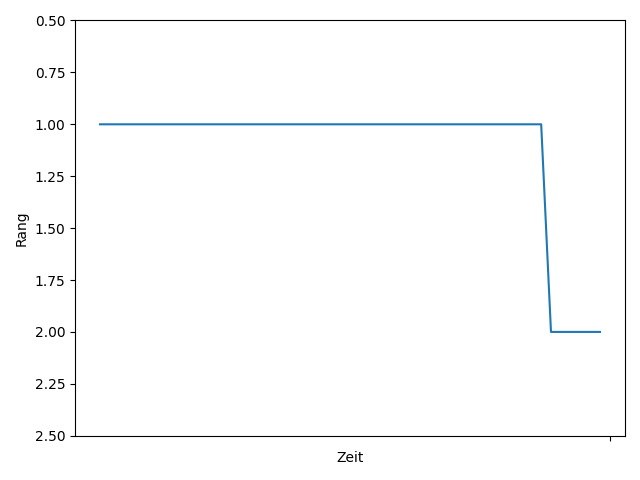
\includegraphics[scale=.25]{JavaTIOBE.png}
        \end{subfigure}
        \begin{subfigure}[h!]{.5\textwidth}
            \caption{Java GitHut 2.0-Index}
            \centering
            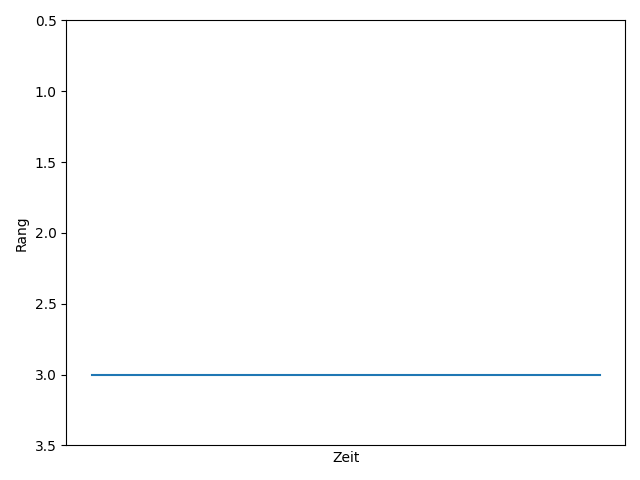
\includegraphics[scale=.25]{JavaGitHut.png}
        \end{subfigure}
    \end{figure}\\
    Der Verlauf im TIOBE Index deutet an, dass nach Java immer weniger gesucht wird. Das kann daran liegen, dass die Sprache nicht mehr so modern und beliebt ist, oder dass sehr viele Entwickler bereits Java kennen. Auf GitHub ist Java seit dem Quartal 03/2015 auf Platz 3.\\
    Letztendlich würde ich sagen, dass Java nicht mehr so gefragt ist, wie es mal war. Da jedoch sehr viele Unternehmen noch Java verwenden, und Java bei Android als noch eine große Rolle spielt, wird Java die nächsten Jahre bis Jahrzehnte weiterhin bestehen.\\\\
    \textbf{Python}\\
    Auch hier liegt das letzte Update in der 18 Monate Grenze. Daher wird der Verlauf der Beliebtheit auch hier graphisch angegeben:
    \begin{figure}[h!]
        \begin{subfigure}[h!]{.5\textwidth}
            \caption{Python TIOBE-Index}
            \centering
            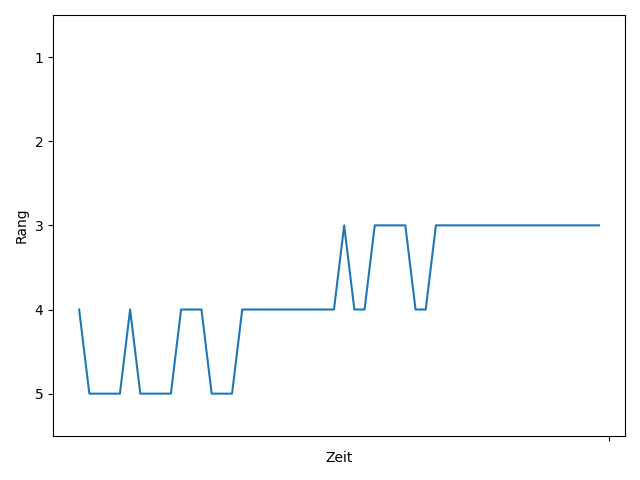
\includegraphics[scale=.25]{PythonTIOBE.png}
        \end{subfigure}
        \begin{subfigure}[h!]{.5\textwidth}
            \caption{Python GitHut 2.0-Index}
            \centering
            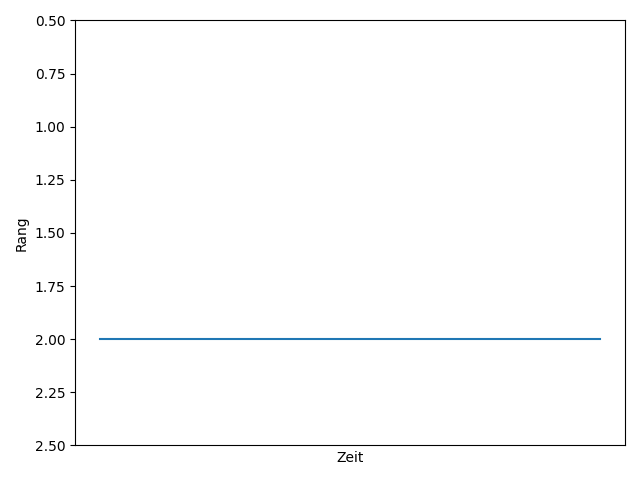
\includegraphics[scale=.25]{PythonGitHut.png}
        \end{subfigure}
    \end{figure}\\
    Wie bei Java ist auch bei Python die Beliebtheit auf GitHub gleich geblieben, nur dass Python mit Platz 2 beliebter ist als Java.\\
    Im TIOBE Index hat die beliebtheit am Anfang zwischen Platz 4 und 5 geschwankt, bi dem späteren Verlauf wurde Python jedoch beliebter, bis sie seit einigen Monaten auf Platz 3 liegt. Ein Grund dürfte die, zur Zeit, sehr hohe Nachfrage nach Python sein.\\
    Da Python immer mehr auf Suchmaschinen gesucht wird und die Beliebtheit bei Pull-Requests auf GitHub die zweithöchste ist, würde ich Python als sehr Zukunftssicher einstufen.\\\\
    \textbf{C$\sharp$}\\
    Da die Vorschauversion keine 18 Monate entfernt veröffentlicht wurde, wird der Beliebtheitsverlauf von C$\sharp$ folgend graphisch dargestellt:
    \begin{figure}[h!]
        \begin{subfigure}[h!]{.5\textwidth}
            \caption{C$\sharp$ TIOBE-Index}
            \centering
            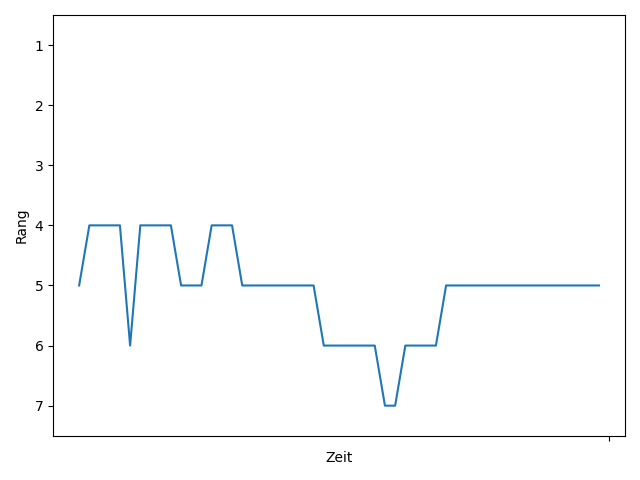
\includegraphics[scale=.25]{CSharpTIOBE.png}
        \end{subfigure}
        \begin{subfigure}[h!]{.5\textwidth}
            \caption{C$\sharp$ GitHut 2.0-Index}
            \centering
            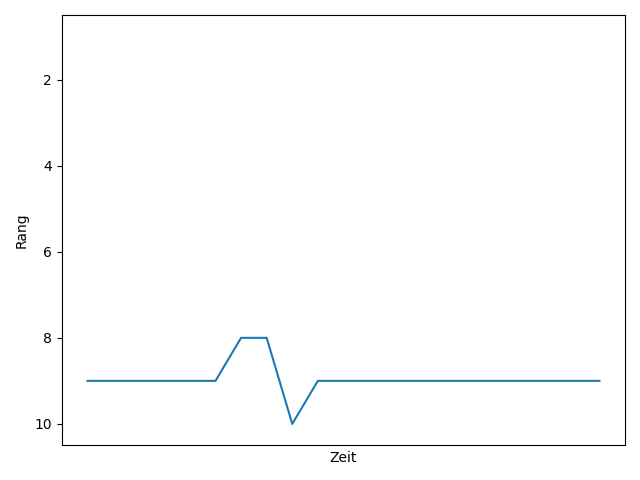
\includegraphics[scale=.25]{CSharpGitHut.png}
        \end{subfigure}
    \end{figure}\\\\
    C$\sharp$ ist zwar Syntax-Technisch sehr ähnlich zu Java, jedoch nicht so beliebt. Nach dem TIOBE Index hat C$\sharp$ bis vor wenige Monate einige Schwankungen von den Suchanfragen her. Es ist bis vor wenige Monate ein ständiges Steigen und Fallen, jedoch hält sich C$\sharp$ insgesamt ungefähr auf Platz 5. Anders sieht es auf GitHub aus. Hier sind sehr wenige Schwankungen. Auch hier bleibt insgesamt der Rang von C$\sharp$ ziemlich gleich, auf Platz 9.\\
    Da C$\sharp$ nicht unbeliebter wird und vor allem sehr viel Verwendung im .NET Framework für die Desktop, Mobile, Web und Spieleentwicklung hat, schätze ich C$\sharp$ als sehr Zukunftssicher ein. Ein Hauptfaktor hierfür ist noch, dass Microsoft, als ein gigantisches Unternehmen, hinter C$\sharp$ steht.\\\\
    \textbf{Visual Basic .NET}\\
    Visual Basic .NET wird nicht mehr weiter betrachtet, da das letzte Update 2 Jahre her ist und die Programmiersprache nicht mehr neue Features bekommt.\\\\
    \textbf{PHP}\\
    PHP ist in der 18 Monatsgrenze des letzten Updates und der Verlauf der Beliebtheit wird auch hier graphisch angezeigt:
    \begin{figure}[h!]
        \begin{subfigure}[h!]{.5\textwidth}
            \caption{PHP TIOBE-Index}
            \centering
            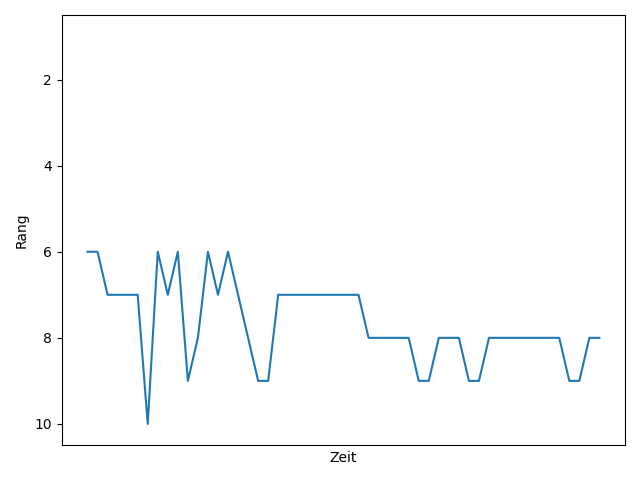
\includegraphics[scale=.25]{PHPTIOBE.png}
        \end{subfigure}
        \begin{subfigure}[h!]{.5\textwidth}
            \caption{PHP GitHut 2.0-Index}
            \centering
            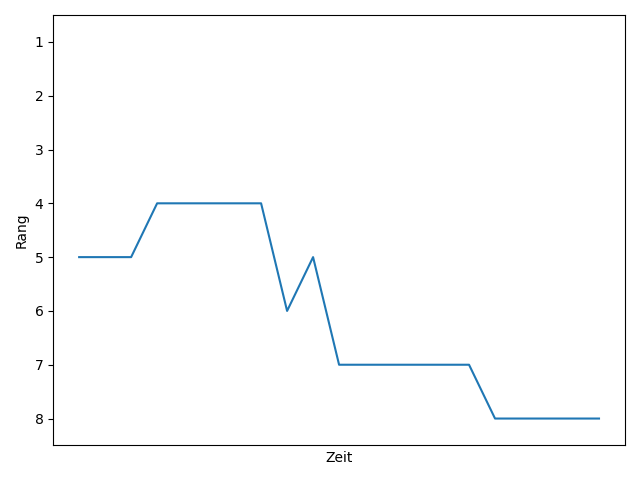
\includegraphics[scale=.25]{PHPGitHut.png}
        \end{subfigure}
    \end{figure}\\
    Bei PHP gibt es im TIOBE Index anfangs starke Schwankungen der Beliebtheit. Nur sind diese Schwankungen bei PHP stärker. PHP fing an auf Platz 6, und schwankt dann zwischen Platz 6 und 10, bis sie letztendlich zwischen Platz 8 und 9 schwankt. Sichtbar ist hier eine sinkende Tendenz der Beliebtheit.\\
    Auch auf GitHub kann sich PHP immer weniger auf hohen Plätzen halten. Die Sprache ist erst leicht beliebter geworden, bis sie letztendlich von Platz 5 am Anfang auf Platz 8 im letzten Quartal abgerutscht ist.\\
    Allerdings wird PHP sehr viel als Backend Sprache auf den Servern eingesetzt.\\
    Ich stufe PHP nicht als ganz Zukunftssicher ein. Sie wird wahrscheinlich noch sehr lange Zeit Updates erhalten, da scheinbar aber immer weniger Entwickler mit PHP arbeiten wollen, sehe ich keine sehr große Zukunft für PHP.\\\\
    \textbf{Delhpi/Object Pascal}\\
    Da das letzte Update über 18 Monate her ist wird Delhpi/Object Pascal nicht mehr vom Beliebtheitsverlauf betrachtet.\\\\
    \textbf{Groovy}\\
    Groovy liegt in der 18 Monate Grenze seit dem letzten Update und der Beliebtheitsverlauf von Groovy wird folgend graphisch angegeben:
    \begin{figure}[h!]
        \begin{subfigure}[h!]{.5\textwidth}
            \caption{Groovy TIOBE-Index}
            \centering
            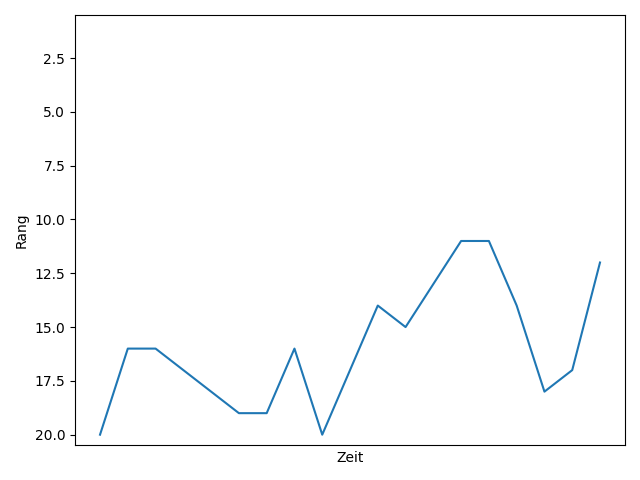
\includegraphics[scale=.25]{GroovyTIOBE.png}
        \end{subfigure}
        \begin{subfigure}[h!]{.5\textwidth}
            \caption{Groovy GitHut 2.0-Index}
            \centering
            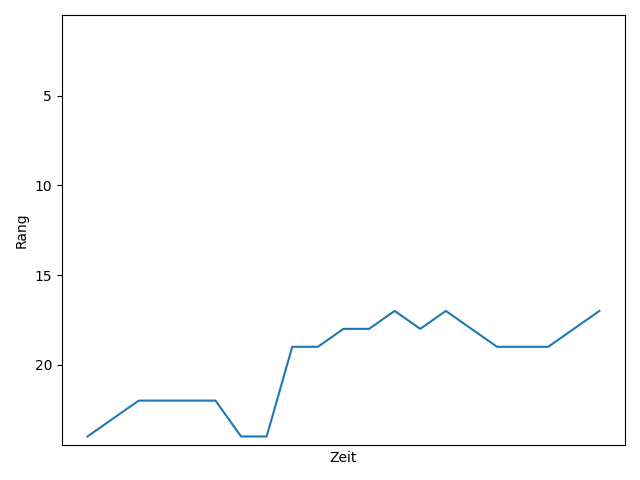
\includegraphics[scale=.25]{GroovyGitHut.png}
        \end{subfigure}
    \end{figure}\\
    Bei Groovy ist der Trend nicht ganz erkennbar.\\
    Der TIOBE Index zeigt am Anfang einen Anstieg der Suchen nach Groovy, danach werden die Anfragen jedoch wieder weniger. Später erreicht Groovy seinen Höhepunkt auf Platz 11, jedoch fällt die Nachfrage direkt wieder und steigt dann wieder auf Platz 12.\\
    Auch auf GitHub steigert Groovy sich vom Platz und fällt wenig später wieder. Dann steigt Groovy wieder, fällt und steigt.\\
    Ich würde dennoch Groovy als Zukunftssicher einstufen, denn insgesamt wurde die Beliebtheit von Groovy nicht schlechter als sie am Anfang war. Sie steigert sich sogar im Vergleich vor 4-5 Jahren. Nach dem TIOBE Index sind es zwar extreme Unterschiede, jedoch ist der Anstieg auf GitHub stärker als der Fall.\\\\
    \textbf{Scala}\\
    Scala liegt mit dem letzten Update in der 18 Monate Grenze. Der Beliebtheitsverlauf wird folgend graphisch dargestellt:
    \begin{figure}[h!]
        \begin{subfigure}[h!]{.5\textwidth}
            \caption{Scala TIOBE-Index}
            \centering
            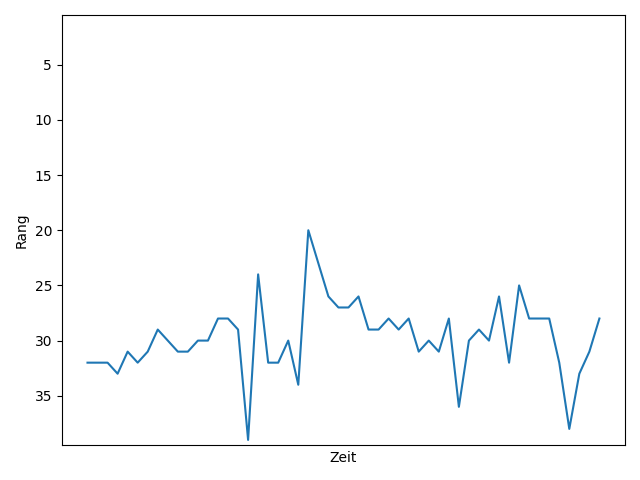
\includegraphics[scale=.25]{ScalaTIOBE.png}
        \end{subfigure}
        \begin{subfigure}[h!]{.5\textwidth}
            \caption{Scala GitHut 2.0-Index}
            \centering
            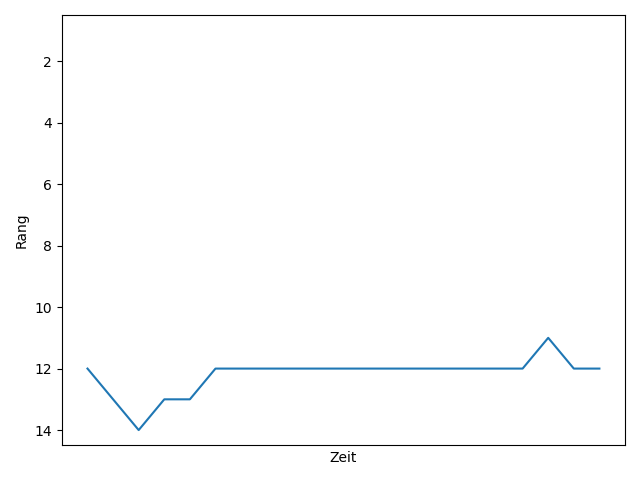
\includegraphics[scale=.25]{ScalaGitHut.png}
        \end{subfigure}
    \end{figure}\\
    In dem TIOBE Index schwankt der Rang von Scala als hin und her.\\
    Anfangs wird Scala beliebter von den Suchanfragen her, dann fällt die Beliebtheit. Dann steigt die Beliebtheit noch höher, und fällt direkt wieder. Zurzeit steigt die Beliebtheit wider, wie lange der Anstieg anhält, ist jedoch nicht klar. Nach dem TIOBE Index ist Scala nicht die beliebteste Sprache, jedoch bleibt der Rang auf die Zeit betrachtet ziemlich gleich.\\
    Scala bewegt sich in dem GitHut Index auf die ganze Zeit gesehen meist auf Platz 12. Es gibt wenige Abweichungen. Damit ist Scala ziemlich stabil von den Pull Requests.\\
    Ich stufe Scala auch als Zukunftssicher ein. Der Grund ist die hohe Stabilität auf GitHub. Die Suchanfragen nach Scala bringen die Sprache zwar ins Schwanken, aber letztendlich ist Scala auch im TIOBE Index Trendmäßig gleichgeblieben.\\\\
    \textbf{Kotlin}\\
    Auch Kotlin liegt in der 18 Monate Grenze seit dem letzten Update und der graphische Verlauf der Beliebtheit wird graphisch dargestellt:
    \begin{figure}[h!]
        \begin{subfigure}[h!]{.5\textwidth}
            \caption{Kotlin TIOBE-Index}
            \centering
            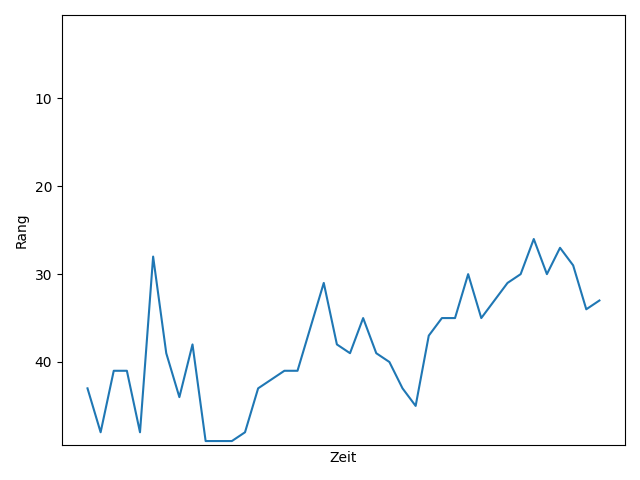
\includegraphics[scale=.25]{KotlinTIOBE.png}
        \end{subfigure}
        \begin{subfigure}[h!]{.5\textwidth}
            \caption{Kotlin GitHut 2.0-Index}
            \centering
            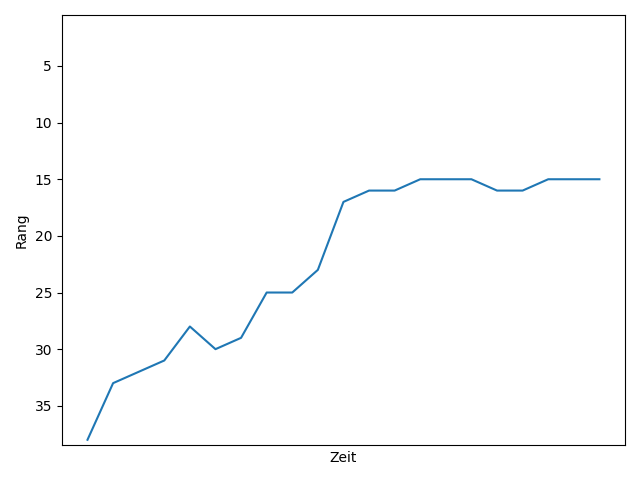
\includegraphics[scale=.25]{KotlinGitHut.png}
        \end{subfigure}
    \end{figure}\\
    Wie bei Scala ist auch bei Kotlin ein dauerhaftes Schwanken im TIOBE Index.\\
    Bei Kotlin hingegen ist der Rang letztendlich wesentlich höher als am Anfang.\\
    Auf GitHub erfreut sich Kotlin immer größerer Beliebtheit. Im Gegensatz zum Anfang hat sich der Rang mehr als verdoppelt und stabilisiert sich letztendlich um den Rang 15.\\
    Durch den letztendlich höheren Rang im TIOBE Index und den viel höheren Rang im GitHut Index stufe ich Kotlin als Zukunftssicher ein.\\\\
    Folgende Programmiersprachen wurden als Zukunftssicher eingeschätzt und werden für die Performanzvergleiche betrachtet:\\
    Java, Python, C$\sharp$, Groovy, Scala und Kotlin.\\\\
    \textbf{Ausführungsgeschwindigkeit}\\
    Wie in \ref{GrundlagenExecutionPerformance} zu erkennen ist, sind ist jede der Programmiersprachen mindestens einmal schneller als die anderen 3.\\
    Da die Ausführungszeit hier unterschiedlich ist und nicht der Ausführungszeitreihenfolge aus der ersten Quelle direkt nachkommt, werde ich eigene Tests schreiben. Diese Tests werden im nächsten Abschnitt genauer beschrieben, nachdem nach bestimmten Bibliotheken gesucht wurde.\\\\
    \textbf{Entwicklungsgeschwindigkeit}\\
    Anhand der gefundenen Bibliotheken aus \ref{GrundlagenEntwicklungsgeschwindigkeit} werden dann Performanzvergleiche geführt. Dazu wird eine Datenbank eingerichtet, welche 10.000 Einträge in einer Tabelle enthält. Anschließend wird diese Tabelle ausgelesen und die Datenbankeinträge in einer Liste gespeichert. Weiterhin wird eine INI Datei mit 4 Kategorien und jeweils 5 Einträgen pro Katergorie erstellt. Diese wird eingelesen, jeder Eintrag in einer Liste gespeichert, der letzte Eintrag jeder Kategorie verändert und wieder zurückverändert.\\
    Die Ausführungsgeschwindigkeit wird mithilfe von der Systemzeit gemessen. Dazu wird die aktuelle Systemzeit vor dem Codeblock gespeichert und diese Zeit von der Systemzeit nach dem Codeblock subtrahiert. Die Programme werden jeweils 50x ausgeführt und der Mittelwert der Ergebnisse genommen.\\
    Für Entwicklungsgeschwindigkeit wird anhand der notwendigen Codezeilen und dem notwendigen Overhead beurteilt.\\\\
    \textbf{Ergebnisse Ausführungsgeschwindigkeits- und Entwicklungsgeschwindigkeitstests}\\
    \textit{Was sind die Ergebnisse?}\\
    Die Tests wurden auf einem Linux Mint 20 Cinnamon Laptop ausgeführt, der folgende Hardware hat:\\
    \textbf{Prozessor:} Intel© Core™ i5-7200U CPU @ 2.50GHz × 2\\
    \textbf{Arbeitsspeicher:} 8GB\\
    \textbf{Grafikkarte:} Intel Corporation HD Graphics 620\\\\
    Die folgende Tabelle zeigt die Ergebnisse der Tests:\\
    \begin{tabular}{|l|l|l|l|}
        \hline
        \textbf{Programmiersprache}&\textbf{Datenbank}&\textbf{INI Datei}&\textbf{Codezeilen gesamt}\\
        \hline
        Java&0,0071 s&0,0025 s&142\\
        \hline
        Python&0,0488 s&0,0264 s&67\\
        \hline
        C$\sharp$&0,0210 s&0,0013 s&134\\
        \hline
        Groovy&0,3625 s&0,0063 s&85\\
        \hline
        Kotlin&0,0086 s&0,0022 s&68\\
        \hline
        Scala&0,0084 s&0,0035 s&106\\
        \hline
    \end{tabular}\\
    Weiterhin wurden die Tests auf einem Windows 10 Computer ausgeführt, welcher folgende Hardware hat:\\
    \textbf{Prozessor:} Intel(R) Core(TM) i5-7500 CPU @ 3.40GHz, 3408 MHz, 4 Kern(e), 4 logische(r) Prozessor(en)\\
    \textbf{Arbeitsspeicher:} 16GB\\
    \textbf{Grafikkarte:} NVIDIA GeForce GTX 1060 6GB\\\\
    Hier sind die Ergebnisse der Geschwindigkeitstests:\\
    \begin{tabular}{|l|l|l|}
        \hline
        \textbf{Programmiersprache}&\textbf{Datenbank}&\textbf{INI Datei}\\
        \hline
        Java&0,0062 s&0,0037 s\\
        \hline
        Python&0,0326 s&0,0191 s\\
        \hline
        C$\sharp$&0,0088 s&0,0029 s\\
        \hline
        Groovy&0,6326 s&0,0049 s\\
        \hline
        Kotlin&0,0066 s&0,0036 s\\
        \hline
        Scala&0,0071 s&0,0039 s\\
        \hline
    \end{tabular}\\
    \textit{Interpretation der Ergsbnisse und beantwortung, welche Programmiersprachen am besten geeignet sind anhand eines Rankings}\\
    Zu erkennen ist, dass Kotlin und Python, bis auf eine Zeile Unterschied, am wenigsten Codezeilen benötigen. Das liegt daran, dass Python keine Sichtbarkeitsmodifier wie public und private hat und Kotlin automatisch getter und setter generiert, welche sich aber nach belieben ersetzen lassen. Groovy hat auch automatisch generierte getter und setter, im Unterschied zu Kotlin können die Felder aber nicht im Methodenaufruf Styl deklariert werden. Scala erlaubt getter Methoden zu schreiben, die keine Funktionsaufrufklammern haben, wodurch auch wenige Codezeilen eingespart werden, auch erlaubt Scala, wie Kotlin, eine Funktionsaufrufklammern Schreibeweise für die Klassenparameter. Am meisten Codezeilen benötigen Java und C$\sharp$, wobei bei C$\sharp$ von der Codingconvention die Methodenklammern in einer neuen Zeile empfohlen werden, was insgesamt 22 Zeilen ausmacht. Diese unterstützen beide keine Funktionsaufrufklammern Schreibweise für Klassenparameter, auch wird keine automatische getter und setter Generierung unterstützt. Jedoch erlaubt C$\sharp$ eine Kurzschreibweise für getter und setter.\\
    Von der Syntax her ist Python eine sehr lesbare Sprache, egal in welchen Programmen, denn die Syntax erzwingt dies. Die anderen haben keine Syntax, die das Einrücken erzwingt.\\
    Einen kleinen, aber doch netter Unterschied, haben Java und C$\sharp$ zu den anderen 4 Programmiersprachen, denn in nur in Java und C$\sharp$ sind die Semikolons notwendig, in den anderen nicht. So entstehen weniger Syntaxfehler.\\
    Java hängt wenigen sehr netten Features gegenüber den anderen Programmiersprachen zurück, dazu zählt die Stringinterpolation, also das Verwenden von Variablen und Funktionsaufrufe innerhalb des Strings, ohne eine String Format explizit machen zu müssen und das überschreiben der Operatoren.\\
    Python, Kotlin und Groovy erlauben Higher Order Functions, also Funktionen, die außerhalb einer Klasse geschrieben werden können. Das ist ein nettes nice to have, denn so sind keine Klassen für einzelne Methoden notwendig.\\\\
    Entwicklungstechnisch sortiere ich die 6 Programmiersprachen deswegen folgend an:\\
    \textbf{1. Python}: Die Higher Order Functions und vor allem die Syntax machen Python zu einer sehr lesbaren Sprache. Neue Klassenvariablen brauchen nicht explizit deklariert werden, diese können auch in einer Methode deklariert werden. Die Kombination macht Python sehr angenehm zum Entwickeln.\\
    \textbf{2. Kotlin}: Das automatische generieren von getter und setter Methoden durch die data class, die extension Methoden wie run, welche einen Codeblock ausführen lässt, als wäre dieser Teil der Objektklasse, machen es nochmal einfacher zu Entwickeln. Ebenfalls macht das weglassen von dem "new" Schlüsselwort eine Objekterzeugung auch angenehmer.\\
    \textbf{3. Groovy}: Die automatische getter und setter machen das Klassenschreiben angenehmer. Ebenfalls, wie in Kotlin, lässt die with Methode einen Codeblock ausführen, als wäre es Teil der Objektklasse. Groovy braucht leider ein Paar mehr Zeilen Code, wodurch es etwas später eingeordet wird.\\
    \textbf{4. C$\sharp$}: Obwohl Scala weniger Codezeilen benötigt und keine Semikolons notwendig sind, ist C$\sharp$ angenehmer zu entwickeln. Die stark verkürzten getter und setter machen Klassen schreiben viel angenehmer.\\
    \textbf{5. Scala}: Wegen dem notwenigen Schreiben von getter und setter macht es das Entwickeln langsamer im Gegensatz zu Platz 1 bis 4, wodurch Scala auf Platz 5 landet.\\
    \textbf{6. Java}: Java hängt den Programmiersprachen in einigen Aspekten nach, darunter automatisch generierte getter und setter, Stringinterpolation und vor allem Operatorenüberschreibung. Deswegen landet Java auf Platz 6.\\\\
    Nach den Ergebnissen der Ausführungszeit ordne ich die Programmiersprachen wie folgt an:\\
    \textbf{1. Java}: Sowohl auf Linux als auch auf Windows werden die Datenbankeinträge schneller gelesen und in ein Objekt reingepackt. Bei dem einlesen der Ini Datei sind C$\sharp$ und Kotlin nur leicht schneller, jedoch erfolgen Datenbankabfragen häufiger als Dateien einlesen.\\
    \textbf{2. Kotlin}: Kotlin ist nur leicht langsamer als Scala im Datenbanktest auf Linux und etwas schneller auf Windows. Im INI Test ist Kotlin jedoch beide Male schneller.\\
    \textbf{3. Scala}: Scala ist nur leicht langsamer als Kotlin im Ini Test und doch wesentlich langsamer als C$\sharp$, jedoch ist Scala auf Linux im Datenbanktest schneller als C$\sharp$ und etwas langsamer auf Windows.\\
    \textbf{4. C$\sharp$}: Auf Linux ist C$\sharp$ wesentlich langsamer als auf Windows bei dem Datenbanktest. Insgesamt ist C$\sharp$ bei diesem Test am Platz 4. Anders sieht es bei dem INI Test aus, denn dort ist C$\sharp$ auf beiden Betriebssystemen am schnellsten. Da jedoch mehr Daten abgefragt werden und die Ausführung auf Linux so lange dauert, was wahrscheinlich daran liegt, dass C$\sharp$ von Microsoft entwickelt wird und es bei Windows für die Entwicklung verwendet wird, wird C$\sharp$ hier eingeordnet.\\
    \textbf{5. Python}: Python braucht zwar beim INI Test auf beiden Betriebssystemen am längsten, jedoch ist Python beim Datenbanktest noch wesentlich schneller als Groovy.\\
    \textbf{6. Groovy}: Groovy braucht bei dem Datenbanktest am längsten, und das mit weitem Abstand. In der Praxis ist diese Zeit viel zu lange.\\\\
    Insgesamt würde ich die Programmiersprachen wie folgt anordnen:\\
    \textbf{1. Kotlin}: Kotlin ist bei der Ausführungsgeschwindigkeit und Entwicklungsgeschwindigkeit auf Platz 2. Kotlin ist nur minimal langsamer als Java, lässt sich aber viel schneller entwickeln.\\
    \textbf{2. Java}: Java ist zwar bei der Entwicklung auf dem letzten Platz, jedoch ist Java von den ganzen Programmiersprachen die schnellste. Die Entwicklung ist zwar nicht so angenehm wie bei den anderen Prorgrammierpsrachen, jedoch sind die meisten Aspekte nice to have Sachen.\\
    \textbf{3. Scala}: Scala ist auf Platz 3 der Ausführungseschwindigkeit und auf Platz 5 bei der Entwicklung. Da die Ausführungsgeschwindigkeit aber entscheidender ist als die Entwicklung, ordne ich Scala hier ein.\\
    \textbf{4. C$\sharp$}: Bei beiden Performanzvergleichen ist C$\sharp$ auf Platz 4. Wenn der Server ein Windows Betriebssystem hat, ist C$\sharp$ sehr nahe an Scala von der Ausführungsgeschwindigkeit dran.\\
    \textbf{5. Python}: Die Entwicklung in Python ist sehr sehr angenehm, jedoch dauert die Ausführung der Programme sehr lange. Das wird daran liegen, dass Python interpretiert wird. Deshalb wird Python hier eingeordnet.\\
    \textbf{6. Groovy}: Die Entwicklung ist auch in Groovy sehr angenehm, jedoch ist die Ausführungsgeschwindigkeit noch langsamer als die von Python bei den Datenbanken, was in der Praxis sehr schlecht ist.\\\\
    Anhand der Anordnung wären die Top 4 Programmiersprachen Kotlin, Java, Scala und C$\sharp$. Da jedoch Kotlin, Scala, Java und Groovy auf der JVM lauffähig sind, wird für den dritten Abschnitt noch Python mitbetrachtet neben den Top 4 Programmiersprachen. Der Grund ist, dass ein Python Framework eventuell etwas Geschwindigkeit aufbauen kann.
    \textit{Entscheidungen, die für die Evaluation vorgenommen wurden, welche die Validität der Regebnisse gefährden können}\\
    Folgende Entscheidungen wurde vorgenommen:
    \begin{enumerate}
        \item Version der Programmiersprache: Bei der Entwicklungszeit spielt die Version der Programmiersprache eine Rolle. Der Grund ist, dass bei neueren Versionen oft neue Features hinzukommen, die die Entwicklungszeit deutlich reduzieren können (z.B. foreach Schleifen anstatt klassische for Schleifen).
        \item Betriebssystem: Das Betriebssystem spielt eine wichtige Rolle: Programmiersprachen, die für die Entwicklung des Betriebssystems verwendet werden, laufen in der Regel schneller als Programmiersprachen, die nicht bei der Betriebssystementwicklung verwendet wurden.
        \item Compiler: Die Wahl des Compilers spielt eine entscheidente Rolle. Denn bei den meisten Skriptsprachen, wie Python, gibt es den Compiler, der offiziell bereitgestellt wird. Aber es gibt auch Compiler von anderen Organisationen, welche z.B. das Just in Time Kompilieren unterstützen. Der Compiler wirkt sich auf die Ausführungsgeschwindigkeiten aus.
    \end{enumerate}
    \newpage\noindent
    %
    %%%%%%%%%%%%%%%%%%%%%%%%%% Auswahl Frameworks %%%%%%%%%%%%%%%%%%%%%%%%%%
    \fancyhead[R]{Auswahl geeigneter Web-Frameworks}
    \section{Auswahl geeigneter Web-Frameworks}
    \label{AuswahlFrameworks}
    In diesem Kapitel werden für die übrigen Programmiersprachen Web Frameworks herausgesucht, welche einen GUI Designer bereitstellen.
    \subsection{Auswahlkriterien}
    Für die Web Framework Auswahl werden folgende Kriterien aus \ref{VorstellungOEP} verwendet: 4 (Zukunftssicherheit des Frameworks), 5 (Schnelle Ausführungseschwindigkeit des Frameworks), 6 (Geringe Entwicklungszeit des Frameworks) und 8 (Anforderungen an das Web Framework).
    \subsection{Vorgehen bei der Auswahl}
    Wie in den anderen Abschnitten, werden auch hier die Kriterien nacheinander abgearbeitet.\\
    Folgendes Vorgehen wird für die einzelnen Schritte vorgenommen:\\
    \textbf{Anforderungen an das Web Framework}\\
    Es werden Web Frameworks mit GUI Designer für die resultierenden Sprachen aus \ref{ProgrammiersprachenEntscheidung} gesucht. Es werden nur Frameworks akzeptiert, welche einen GUI Designer direkt bereitstellen oder eine Erweiterung des Frameworks einen Designer bereitstellt.\\
    \textbf{Zukunftssicher des Frameworks}\\
    Für jedes gefundene Web Framework wird herausgesucht, ob das letzte Update in den letzten 12 Monaten war. Weiterhin wird geschaut, wer dieses Framework entwickelt und welche Unternehmen dieses Framework verwenden.\\
    Anhand der gefundenen Informationen wird eine Prognose abgegeben, ob dieses Framework zukunftssicher scheint.\\
    \textbf{Schnelle Ausführungseschwindigkeit und Geringe Entwicklungszeit des Frameworks}\\
    Die Performanz für die übrigen Frameworks wird auch hier anhand von einem kleinen Programm getestet.\\
    Hierfür wird eine neue Datenbank aufgesetzt, welche 3 Tabellen mit je 4 Spalten hat. Es wird weiterhin eine INI Datei geschrieben, welche verschiedene Konfigurationen speichert. Diese Konfigurationen enthalten einen Namen, eine Beschreibung und einen SQL Statement.\\
    Auf der Webseite bekommt man die Option eine Konfiguration auszuwählen. Dann wird einem der Name und Beschreibung angezeigt.Ebenfalls werden die Daten aus der Datenbank ausgelesen und angezeigt. Es gibt die Option nur eine bestimmte Anzahl an Daten zu holen.\\
    Anschließend werden die Web Frameworks nach der Ausführungseschwindigkeit und Entwicklungsgeschwindigkeit bewertet.
    \subsection{Entscheidung}
    \textbf{Anforderungen an das Web Framework}\\
    Hier gibt es keine Interpretation. Die gefundenen Frameworks sind in \ref{GrundlagenWebFrameworksWithGUIDesigner} zu finden.\\
    \textbf{Zukunftssicher des Frameworks}\\
    \indent\textbf{JSF} JavaServer Faces stufe ich als nicht Zukunftssicher ein. Der Grund ist, dass das letzte Update im April 2017 war. Zwar lässt sich das Framework noch verwenden, jedoch werden Bugs usw. wahrscheinlich nicht mehr behoben.\\
    \indent\textbf{Vaadin} Vaadin stufe ich als Zukunftssicher ein, denn das letzte Update ist erst wenige Tage her. Außerdem wird Vaadin unter anderem von Volkswagen und Dell verwendet, welche ein sehr großes Interesse an einer Weiterentwicklung haben. Weiterhin ist Vaadin in der Kostenlosen Version Open Source, wodurch eine Community auch die Option hat das Framework weiterzuentwickeln.\\
    \indent\textbf{KVision} KVision stufe ich als nicht Zukunftssicher ein. Zwar war das Update auch erst wenige Tage her, jedoch habe ich keine Unternehmen gefunden, welche das Framework verwenden. Auch wird das Framework von nur einer Person entwickelt und wenn diese die Entwicklung aufgibt, ist das Framework sehr wahrscheinlich tot.\\
    \indent\textbf{Codename One} Codename One stufe ich zwar als Zukunftssicher ein, weil es von Ex Sun/Oracle Mitarbeitern entwickelt wurde, die in einem Unternehmen sind und das letzte Update in IntelliJ vor ca. 6 Monaten war. Jedoch kann das Framework nur verwendet werden, wenn das Plugin installiert wurde. Bei Netbeans hingegen ist das Update schon über 21 Monate her, was die Updates erhalten schwieriger macht.\\
    \indent\textbf{WebBot} WebBot stufe ich ebenfalls als nicht Zukunftssicher ein. Der Grund ist, wie bei KVision, dass zwar das letzte Update nicht so lange her ist, jedoch wird es von nur einer Person entwickelt und es sind keine Unternehmen bekannt, die dieses Framework nutzen.\\
    \indent\textbf{Anvil} Wie Codename One stufe ich zwar Anvil als Zukunftssicher ein, weil das letzte Update im August war. Ebenfalls wird es von ein Paar Unternehmen verwendet. Jedoch lassen sich Seiten nur per Drag und Drop über deren Online Designer entwickeln. Das Runtime Environment lässt zwar das Hosten auf dem eigenen Rechner zu, jedoch steht der Designer dann nicht mehr bereit.\\
    \indent\textbf{Widgy(Django)} Hier ist es eine schwere Entscheidung. Django ist das wohl größte Python Web Framework, welches unter anderem von Instagram, Spotify und Youtube verwendet wird. Dieses wird sehr wahrscheinlich noch sehr lange leben. Anders sieht es bei der Erweiterung Widgy aus. Diese hat seit über einem Jahr kein Update mehr erhalten. Es können möglicherweise schon alle Funktionalitäten programmiert sein, aber eine Software braucht immer Pflege, um weiterleben zu können. Wegen wahrscheinlich keinen Updates für Widgy werden keine Bugs mehr behoben, die in dem Designer auftreten. Deshalb stufe ich diese Kombination als nicht zukunftssicher ein.\\
    \indent\textbf{Wisej} Dieses Framework wird von einem Unternehmen entwickelt, welches jedoch kleiner ist. Das letzte Update ist erst ca. 1 Monat her und das Framework wird unter anderem von Goodyear verwendet. Das Framework ist leider auch etwas unbekannt, wahrscheinlich auch weil es relativ neu ist. Ich stufe Wisej als Zukunftssicher ein mit dem Hintergedanken, dass ein anderes Framework mit gleich oder leicht schwächeren Performanzdaten bevorzugt wird bei der Entscheidung.\\
    \indent\textbf{WebForms} WebForms wurde von Microsoft entwickelt. Leider habe ich kein Datum gefunden, wann das letzte Update war. Da dieses in .NET integriert ist, wird es wohl noch länger leben. Jedoch habe ich ebenfalls kein Unternehmen gefunden, welches dieses Framework verwendet.\\
    \indent\textbf{Radzen(Blazor)} Das Framework Blazor wurde ebenfalls von Microsoft entwickelt, ist Open Source und in .NET enthalten. Die Erweiterung Radzen ist von einem kleinen Unternehmen entwickelt. Blazor hat im April 2020 das letzte Update erhalten, Radzen vor wenigen Tagen. Das Framework selbst wird unter anderem von Durstexpress verwendet, Radzen soll von Dell und Microsoft verwendet werden. Da Blazor noch Updates zu erhalten scheint und Radzen sehr viele in kurzer Zeit stufe ich diese Kombination als Zukunftssicher ein.\\
    Übrig bleiben also Vaadin, Wisej und Radzen.\\\\
    \textbf{Schnelle Ausführungseschwindigkeit und Geringe Entwicklungszeit des Frameworks}\\
    Da nur 3 Frameworks übrig bleiben verzichte ich in diesem Abschnitt auf die Performanztests und integriere diese in den nächsten Abschnitt, in welchem ein Modul nachprogrammiert wird.
    \newpage\noindent
    %
    \fancyhead[R]{Entwicklung eines Moduls in verschiedenen Frameworks}
    \section{Entwicklung eiens Moduls in verschiedenen Frameworks}
    \label{Neuentwicklung}
    \subsection{Frameworks, mit denen ein Modul entwickelt wird}
    \textbf{Vaadin:} Da Vaadin auf der JVM läuft, ist eine Entwicklung mit Java, Scala und Kotlin denkbar. Da der Designer jedoch Java Klassen ausgibt, wird das Modul mit Java Entwickelt.\\
    \textbf{Wisej:} Da ich die Bachelorarbeit an einem Linux PC schreibe und der Wisej Designer zur Zeit nur mit Visual Studio funktioniert wird die Entwicklung mit Wisej leider ausfallen.\\
    \textbf{Radzen(Blazor):} Da Wisej ausfällt und Blazor Server und Client Seitig programmiert werden kann, wird das Modul sowohl Server Seitig als auch Client Seitig entwickelt.
    \subsection{Evaluation der Modulentwicklung}
    \textit{Welche Forschungsfrage soll beantwortet werden?}\\
    Die Entwicklung eines Moduls in den 2 Frameworks dient zur Untersuchung, mit welchem Framework eine Entwicklung potenziell am schnellsten erfolgen kann. Weiterhin wird neben der Entwicklungszeit auch die Ausführungszeit gemessen. Dazu zählt die Ausführungszeit auf dem Server, dem Client und der Kommunikation zwischen Server und Client.\\
    \textit{Was ist das Setup?}\\
    Für die Entwicklung der Module wird eine MySQL/MariaDB Datenbank aufgesetzt. Weiterhin wird die Entwicklungsumgebung IntelliJ IDEA für die Entwicklung von dem Modul mit Vaadin verwendet. Für die Entwicklung mit Radzen für die Server und Client Seite werden der Radzen Designer und die Entwicklungsumgebung Rider verwendet.\\
    \textit{Wie wird die Evaluation durchgeführt?}\\
    Eine MySQL/MariaDB Datenbank wird aufgesetzt, welche von den 3 Projekten genutzt wird. Diese Datenbank enthält 2 Tabellen. Eine Tablle Person, welche Informationen zu einer Person speichert und einer Tabelle Meeting, welche ein Treffen zwischen zwei Personen speichert.\\
    In der Personen Tabelle werden 10000 Datensätze gespeichert, in der Meeting Tabelle werden 5000 Treffen gespeichert.\\
    Weiterhin wird eine INI Datei erstellt, welche 2 SQL Abfragen und 3 Filter Optionen enthält. Beide SQL Abfragen enthalten ein Platzhalter, welche zur Laufzeit ersetzt werden, sodass ein eine gültige Abfrage zustande kommt. Die Filter Optionen enthalten einen Namen, Default Werte für die Filterung und den Platzhalternamen von der SQL Abfrage.\\
    Die Entwicklung des Moduls selbst sieht wie folgt aus:\\
    Es wird eine Seite erstellt, welche 2 Tabellen und eine Filteroption enthält. Die eine Tabelle soll die Personen aus der Datenbank anzeigen. Sie enthält die Spalten Vorname, Nachname, PLZ, Stadt und Bundesland. Die höhe soll 50\% sein und die Breite 60\%. Rechts neben dieser Tabelle sollen die Filteroptionen stehen. Dabei gibt es die Option nach der Stadt, der PLZ und dem Bundesland zu filtern, oder eine Kombination.\\
    Die einzelnen Filter enthalten einen Text, welcher angibt was gefiltert wird. Die Eingabe soll ein Dropdown Menü sein, bei welchem sich zusätzlich der aktuelle Wert durch Schreiben verändern lässt. Unter den 3 Filtern ist ein Button zur Bestätigung. Diese Filterspalte soll eine Breite von 40\% haben und eine Höhe von 50\%.\\
    Die letzten 50\% der Seite soll die zweite Tabelle einnehmen. Diese zeigt die Meetings mit den Spalten Person und Datum. Person zeigt den Vor- und Nachnamen inklusive PLZ und Wohnort an, z.B. Jonas Borgerding (35260 Stadtallendorf). Das Datum zeigt das Datum des Treffens an.\\
    Daten werden für die erste Tabelle nur angezeigt, wenn der Filter Button betätigt wird. Es werden alle Daten sofort geladen, jedoch auf mehrere Seiten in der Tabelle aufgeteilt. Pro Seite sollen 10 Personen angezeigt werden.\\
    Wenn eine Person in der ersten Tabelle ausgewählt wird sollen alle Treffen mit einer anderen Person in der zweiten Tabelle angezeigt werden. Dafür wird die jeweils andere Person in der Tabelle inklusive den Treffdatum angezeigt. Die Einträge werden auch in der zweiten Tabelle auf Seiten eingeteilt.\\
    Für beide Tabellen soll es die Option geben die Einträge nach den einzelnen Spalten zu sortieren.\\
    Außerdem soll links ein Menü sein, welches alle Seiten der Anwendung anzeigt. Diese hat in diesem Fall jedoch nur eine Seite.\\
    Es soll außerdem noch ein Footer und ein Header bei der Webseite bereitgestellt werden, in welchem zusätzliche Informationen angezeigt werden können.\\
    Für den Vergleich wird betrachtet, wie einfach die Erstellung eines Projektes, die Bedienung des Designers und die eventuelle Erweiterung um benötigte Komponenten war. Außerdem wird die Downloadgröße in 2 verschiedenen Browsern (Google Chrome und Firefox) für die Pure Webseite ohne Daten herausgesucht. Diese Information ist hilfreich, denn der Nutzer soll nicht zu lange warten müssen um die Anwendung bedienen zu können. Außerdem wird die Downloadgröße in den Browsern für die Pure Webseite ohne Datenabfrage herausgesucht, denn diese ist für die Verfügbarkeit der Anwendung nach dem Starten verantwortlich. Für die Downloadgeschwindigkeit und Downloadgröße wird die Untersuchung jeweils 20 Mal gemacht und der Durchschnitt genommen.\\
    \textit{Ergebnisse}\\
    \textbf{Radzen Server-Side:}\\
    1. Entwicklung: Die Erstellung eines Projektes erfolgt über den Radzen Designer. Es werden Informationen über das Projekt angegeben. Bei bestätigung wird ein vollständiges .NET Projekt erstellt, welches anschließen auch in Visual Studio, Rider usw. geöffnet werden kann.\\
    Bei dem angelegten Projekt werden direkt 2 Layouts erstellt. Eins für eine Login Seite und ein Layout mit einem Footer und Header und einem Menü zum Auswählen der einzelnen Seiten der Anwendung.\\
    Neben den Layout gibt es die Seiten(Pages), die den eigentlichen Inhalt liefern. Es können auch zwischen Vordefinierten Pages eine ausgewählt werden, auf welcher man aufbauen kann. Darunter sind einige Seiten, bei denen Daten aus einer Datenbank angezeigt werden können. Der Designer kümmert sich um die Abfragen und dem generieren der einzelnen Spalten für die Datenanzeige.\\
    Allerdings sind für das Projekt eigene Anfrage formuliert, welche beim Entwickeln dann doch selbst in die Tabelle gebracht werden müssen.\\
    Wählt man die Komponente DataGrid aus und platziert sie auf der Seite sieht man im Designer Optionen zum Anpassen. Über diese Optionen lässt sich das Aussehen verändern, Spalten definieren usw.\\
    Weiterhin lassen sich über Events schon Funktionen aufrufen, auch eigen geschriebene Funktionen erkennt der Designer. Dies erlaubt mir die Events vom DataGrid und einem Button zu nutzen, um die eigens geschrieben Funktionen zur Datenbankabfrage aufzurufen.\\
    Da Radzen keine Komponente bereitstellt, die per Dropdown eine Option wählen lässt und der Nutzer diese per Schreiben verändern kann, muss eine solche Komponente selbst geschrieben werden.\\
    Dafür habe ich in Rider die Radzen Bibliothek verwendet. In einer .razor Datei habe ich von Radzen das Label, die Textbox und das DropDown verwendet, um das Aussehen zu erhalten. Blazor erlaubt die Übergabe von Parametern an eine Komponente. Diese erlaubt mir, die eigens geschrieben Komponente für die 3 Filter wiederzuverwenden.\\
    Im Designer konnte die eigene Komponente per HTML Element in die Seite gebracht werden. Dieses HTML Element von Radzen erlaubt es eigenen html zu schreiben, der in der Seite verwendet wird. Zusammen mit der Blazor For-Schleife und der eignene Komponente konnten die aus der INI Datei gelesenen Filter einfach in die Seite integriert werden.\\
    2. Downloadgeschwindigkeit und Downloadgröße: TODO
    \newpage\noindent
    %
    \fancyhead[R]{Entscheidung für ein Framework}
    \section{Entscheidung für ein Framework}
    \label{Entscheidung}
    \newpage\noindent
    %%%%%%%%%%%%%%%%%%%%%%%%%%Technologieplattform%%%%%%%%%%%%%%%%%%%%%%%%%%
    % \fancyhead[R]{Auswahl der Technologieplattform}
    % \section{Auswahl der Technologieplattform}
    % \subsection{Einleitung}
    % \label{einleitungTechnologiePlattformen}
    % In dem ersten Teil dieser Bachelorthesis wird untersucht für welche Technologieplattform entwickelt werden sollte, damit eine erste Eingrenzung von allen möglichen Entwicklungsmöglichkeiten gemacht werden kann.\\
    % Als Kriterien für die Neuentwicklung gelten:
    % \begin{enumerate}
    %     \item Verfügbarkeit auf allen Betriebssystemen, die eine Benutzeroberfläche und einen Browser haben, wie Beispielsweise Linux, Blackberry und Windows.
    %     \item Keine App-Store Abhängigkeiten, da in der Regel kein Internet auf den Endgeräten verfügbar ist.
    %     \item Effiziente, d.h. schnelle und kostengünstige, Entwicklung, Wartung und Pflege, z.B. soll die Installation beim möglichst schnell, einfach und unabhängig von anderen Systemen sein.
    % \end{enumerate}
    % Da keine direkten Funktionalitäten eines Betriebssystems für die Neuentwicklung bekannt sind und die Endnutzergeräte in einem lokalen Netzwerk sind, ist eine Web Entwicklung nicht ausschließbar.
    % Daher werden folgende Technologieplattformen untersucht:
    % \begin{enumerate}
    %     \item Native Anwendungen
    %     \item Cross-Platform Anwendungen
    %     \item Web Anwendungen
    %     \item Hybride Anwendungen
    % \end{enumerate}
    % Dabei wird für jede Technologieplattform eine kurze Einleitung gegeben und einige Merkmale genannt. Anschließend werden einige Vor- und Nachteile zu den jeweiligen Technologieplattformen genannt.\\
    % \indent Nachdem die Technologieplattformen vorgestellt wurden, wird untersucht, ob und inwieweit die Technologieplattformen die jeweiligen Kriterien erreichen. Am Ende wird eine Technologieplattform ausgewählt, die die Kriterien am besten Erfüllt, vor allem aus dem Wirtschaftlichen Aspekt.\\
    % \indent Informationen über die jeweiligen Technologieplattformen werden über die Suchmaschine "Google" gesucht. Dafür werden folgende Suchbegriffe, getrennt und mit "definition", "advantages" und "disadvantages" am Ende, verwendet:\begin{enumerate}
    %     \item Native Development
    %     \item Cross Platform Development
    %     \item Web Development
    %     \item Hybride Development
    % \end{enumerate}
    % \newpage
    % \subsection{Fazit und Entscheidung}
    % Untersuchung der in \ref{einleitungTechnologiePlattformen} formulierten Kriterien:\\\\
    % \textbf{\textit{Verfügbarkeit auf allen Betriebssystemen mit einer Benutzeroberfläche und einen Browser:}}\\
    % Im Grunde decken alle 4 Technologieplattformen alle Betriebssysteme ab. Jedoch gibt es einen Unterschied vom Aufwand her:\\
    % \indent Bei der nativen Entwicklung muss für jedes Betriebssystem jeweils eine Anwendung geschrieben werden, was zu erhöhten Entwicklungskosten führt.\\
    % \indent Bei der Cross-Platform Entwicklung werden mit einem einzigen Projekt mehrere Betriebssysteme abgedeckt. Hier ist das schreiben von einer bis sehr wenigen Anwendungen notwendig.\\
    % \indent In der Web Entwicklung muss das Projekt nur einmal geschrieben werden und ist dann auf allen Betriebssystemen über einen Browser verfügbar.\\
    % \indent Auch bei der Hybriden Entwicklung werden alle Betriebssysteme abgedeckt. Es muss für jedes einzelne Betriebssystem eine native Anwendung erstellt werden, in welche eine Website eingebunden wird.\\
    % \indent $\Rightarrow$ Hier haben die Cross-Platform und Web Entwicklung einen deutlichen Vorteil gegenüber der hybriden und nativen Entwicklung.\\\\
    % \textbf{\textit{Keine App-Store-Abhängigkeiten:}}\\
    % Hier gibt es einen kleinen Unterschied:\\
    % \indent Auf Desktop Geräten (PC, Laptop) können Programme z.B. einem USB-Stick installiert werden. Somit ist eine Offline Installation für alle 4 Plattformtechnologien auf einem Desktop Geräten ohne Probleme möglich.\\
    % \indent Jedoch ist dies bei mobilen Geräten (Smartphone, Tablet) nicht so einfach möglich. Denn dort werden Apps in der Regel über den jeweiligen Store installiert. Es gibt aber Möglichkeiten Apps ohne den Store zu installieren. Diese sind jedoch nicht so trivial wie für Desktop Geräten.\\
    % \indent $\Rightarrow$ Hier liegt der Vorteil bei den Desktop-Geräten, da hier problemlos die Anwendung installiert werden kann. Bei mobilen Geräten ist dies unter umständen Möglich, jedoch nicht elegant.\\\\
    % \textbf{\textit{Effiziente Entwicklung, Wartung und Pflege}}\\
    % Der Unterschied ist hier sehr markant:\\
    % \indent Bei der nativen-, cross-platform- und hybriden-Entwicklung werden jeweils Anwendungen für die verschiedenen Betriebssysteme erstellt. Bei der Erstinstallation der Anwendung muss diese auf jedes Gerät installiert werden, was sehr viel Zeit benötigt. Auch bei jedem Update muss auf jedem Gerät das Update installiert werden, was wiederum so viel Zeit benötigt.\\
    % \indent Einen klaren Vorteil hat hier die Web-Entwicklung, denn dort muss die Anwendung nur einmal installiert werden(auf dem Server) und ist auf allen Geräten über den Browser zugänglich.\\
    % \indent Bei der Pflege ist bei der nativen Entwicklung am meisten Aufwand zu betreiben, da dort jedes einzelne Projekt weiterentwickelt werden muss.\\
    % \indent Die Cross-Platform-, Hybride- und Web-Entwicklung benötigen in der Regel nur eine Entwicklung, was Zeittechnisch ein klarer Vorteil gegenüber der nativen Entwicklung ist.\\
    % \indent $\Rightarrow$ Die Web-Entwicklung ist Installtions- und Wartungstechnisch den anderen Optionen Kostentechnisch überlegen. Pfelegetechnisch ist nur die native Entwicklung nicht so optimal.\\\\
    % \indent$\Rightarrow$ Zusammengefasst ist die Web-Entwicklung die beste Option für eine Neuentwicklung. Sie ist zwar oft etwas etwas langsamer als eine native Anwendung, jedoch liegt dies unter anderem an der Kommunikation zwischen dem Server und dem Client. Allerdings sind nicht starke Rechner für die Clients notwendig, sondern "nur" ein starker Server. Dieser kann die Website schneller erstellen und dadurch etwas Geschwindigkeit aufholen. Vor allem wird durch die Web-Entwicklung eine Plattformunabhängigkeit geschaffen, die alle möglichen Betriebssysteme mit einem Browser direkt unterstützt. Mit der Plattformunabhängigkeit kommen geringere Entwicklungskosten als bei nativen und hybriden Entwicklungen. Auch sind die Kosten für die Installation und Wartung beim Kunden viel geringer, da nur 1 Rechner die neuere Version braucht. Ein Offline-Installtion ist auch möglich, da der Server in der Regel ein Desktop Computer ist.\newpage
    %%%%%%%%%%%%%%%%%%%%%%%%%%Sprachauswahl%%%%%%%%%%%%%%%%%%%%%%%%%%
    % \section{Auswahl geeigneter Programmiersprachen}
    % \fancyhead[R]{Auswahl geeigneter Programmiersprachen}
    % \subsection{Einleitung}
    % Dieser Teil befasst sich mit der Auswahl von geeigneten Programmiersprachen, für welche im nächsten Schritt Web-Frameworks herausgesucht werden.\\
    % Hier findet eine erste Selektion anhand binärer Kriterien statt, um bereits Programmiersprachen filtern zu können. Im Anschluss werden die übrigen Programmiersprachen anhand von nicht-binären Kriterien weiter gefiltert, bis nur noch ca. 5 Sprachen übrig bleiben.
    % \subsection{Binäre Filterung}
    % \subsubsection{Einleitung}
    % Für die binäre Filterung werden folgende Kriterien verwendet:
    % \begin{enumerate}
    %     \item Die Programmiersprachen ist unter den Top 20 Sprachen in dem TIOBE Index (siehe \ref{GrundlagenTIOBE}) von Dezember 2019 bis Oktober 2020 oder unter den Top 20 Programmiersprachen in GitHut 2.0 in den Quartalen Q4/2019 bis Q3/2020.
    %     \item Die Programmiersprache ist eine "Hochsprache", wie Beispielsweise Java, aber nicht Assembler
    %     \item Die Programmiersprache ist für die Web-Entwicklung geeignet und es gibt mindestens 1 Web-Framework oder eine Erweiterung eines Web-Frameworks, welches einen graphischen Designer bereitstellt
    % \end{enumerate}
    % Die Kriterien werden in der genannten Reihenfolge nacheinander abgearbeitet.
    % Für die Informationssuche wird wiederum die Suchmaschine "Google" verwendet. Es wird für die Programmiersprachensuche folgendes gesucht: "TIOBE index", "Time machine" und "GitHut 2.0".\\
    % Über die \nameref{timeMachine} werden die TIOBE Indizes von Dezember 2019 bis September 2020 herausgesucht.\\
    % Der TIOBE Index wird für Programmiersprachensuche verwendet, da dieser angibt, wie oft nach einer bestimmten Programmiersprache gesucht wird. Dieser lässt sich verwenden um herauszufinden welche Programmiersprachen für ein neues Projekt verwendet werden sollten. \cite{TIOBE Index}\\
    % Da der TIOBE Index nur die Suchanfragen in Suchmaschinen berücksichtigt und nicht wie viel die einzelnen Programmiersprachen in Projekten verwendet werden, wird zusätzlich noch GitHut 2.0 verwendet. GitHut 2.0 führt ein Ranking von der Verwendung der Programmiersprachen auf GitHub. Je mehr eine Programmiersprache in Repositories verwendet wird(neue Projekte, Commits etc.), desto weiter oben ist diese im Ranking. \cite{GitHut 2.0}\\
    % Da beide Statistiken alleine nicht aussagekräftig sind, wird die Kombination aus beiden genommen. Damit erhalten wir eine Liste von Programmiersprachen, die in den letzten Monaten sowohl viel gesucht wurden als auch viel verwendet wurden.\\
    % Um das \nameref{programmingLanguageLevel} der Programmiersprachen aus dem vorherigen Schritt herauszufinden, wird für jede Programmiersprache folgendes gesucht: "$<$Programmiersprache$>$ programming language level". Es werden nur Programmiersprachen akzeptiert, die als "Hochsprache" eingeordnet sind.\\
    % Es werden nur "Hochsprachen" für die Framework-Suche betrachtet, da diese eine höhere Abstraktion haben und dadurch einfacher zu lernen sind und es einfacher ist, in diesen etwas zu Entwickeln. "Hochsprachen" werden mehr für die Web Entwicklung eingesetzt als "niedrigere" Programmiersprachen, da es meistens nicht notwendig ist die letzte kleine Performanz rauszuholen. \cite{High level Low level languages}\\
    % Das Herausfiltern von Programmiersprachen, die kein Web Framework bereitstellen oder eins bereitstellen, aber keinen \nameref{nativeApplicationUI} Designer direkt oder über eine Erweiterung bereitstellen, erfolgt, indem für jede noch übrige Programmiersprache jeweils nach "$<$Programmiersprache$>$ Web Framework visual Designer", "$<$Programmiersprache$>$ Web Framework wysiwyg" und "$<$Programmiersprache$>$ Web Framework Drag and Drop" gesucht wird. Es werden nur Programmiersprachensuchen mit mindestens einem Web Framework, für welches es einen Designer gibt, übernommen. Falls in keinem der Suchergebnisse von Seite 1 bis 3 ein Web Framework mit einem Designer erwähnt wird, nehme ich an, dass es keines gibt.
    % \subsubsection{Programmiersprachen aus dem TIOBE Index und GitHut}
    % \label{programmingLanguagesTIOBEGitHut}
    % Nachfolgend werden alle Programmiersprachen von Dezember 2019 bis Oktober 2020 vom TIOBE Index aufgelistet:\\
    % \begin{tabularx}{\textwidth}{|l|X|c|}
    %     \hline
    %     \textbf{Monat Jahr}&\textbf{Programmiersprachen}&\textbf{Link}\\
    %     \hline
    %     \textbf{Dezember 2019}&Java, C, Python, C++, C$\sharp$, Visual Basic .NET, JavaScript, PHP, SQL, Swift, Ruby, Delphi/Object Pascal, Objective-C, Assembly Language, Go, R, MATLAB, D, Visual Basic, Perl&\cite{TIOBE Index 12.2019}\\
    %     \hline
    %     \textbf{Januar 2020}&Java, C, Python, C++, C$\sharp$, Visual Basic .NET, JavaScript, PHP, Swift, SQL, Ruby, Delphi/Object Pascal, Objective-C, Go, Assembly Language, Visual Basic, D, R, Perl, MATLAB&\cite{TIOBE Index 01.2020}\\
    %     \hline
    %     \textbf{Februar 2020}&Java, C, Python, C++, C$\sharp$, Visual Basic .NET, JavaScript, PHP, SQL, Swift, Go, Assembly language, R, D, Ruby, MATLAB, PL/SQL, Delphi/Object Pascal, Perl, Objective-C&\cite{TIOBE Index 02.2020}\\
    %     \hline
    %     \textbf{März 2020}&Java, C, Python, C++, C$\sharp$, Visual Basic .NET, JavaScript, PHP, SQL, Go, R, Assembly language, Swift, Ruby, MATLAB, PL/SQL, Perl, Visual Basic, Objective-C, Delphi/Object Pascal&\cite{TIOBE Index 03.2020}\\
    % \end{tabularx}
    % \begin{tabularx}{\textwidth}{|l|X|c|}
    %     \hline
    %     \textbf{April 2020}&Java, C, Python, C++, C$\sharp$, Visual Basic, JavaScript, PHP, SQL, R, Swift, Go, Ruby, Assembly language, PL/SQL, Perl, Objective-C, MATLAB, Classic Visual Basic, Scratch&\cite{TIOBE Index 04.2020}\\
    %     \hline
    %     \textbf{Mai 2020}&C, Java, Python, C++, C$\sharp$, Visual Basic, JavaScript, PHP, SQL, R, Swift, Go, MATLAB, Assembly language, Ruby, PL/SQL, Classic Visual Basic, Perl, Scratch, Objective-C&\cite{TIOBE Index 05.2020}\\
    %     \hline
    %     \textbf{Juni 2020}&C, Java, Python, C++, C$\sharp$, Visual Basic, JavaScript, PHP, R, SQL, Swift, Go, Ruby, Assembly language, MATLAB, Perl, PL/SQL, Scratch, Classic Visual Basic, Rust&\cite{TIOBE Index 06.2020}\\
    %     \hline
    %     \textbf{Juli 2020}&C, Java, Python, C++, C$\sharp$, Visual Basic, JavaScript, R, PHP, Swift, SQL, Go, Assembly language, Perl, MATLAB, Ruby, Scratch, Rust, PL/SQL, Classic Visual Basic&\cite{TIOBE Index 07.2020}\\
    %     \hline
    %     \textbf{August 2020}&C, Java, Python, C++, C$\sharp$, Visual Basic, JavaScript, R, PHP, SQL, Go, Swift, Perl, Assembly language, Ruby, MATLAB, Classic Visual Basic, Groovy, Objective-C, Rust&\cite{TIOBE Index 08.2020}\\
    %     \hline
    %     \textbf{September 2020}&C, Java, Python, C++, C$\sharp$, Visual Basic, JavaScript, PHP, R, SQL, Go, Swift, Perl, Assembly language, Ruby, MATLAB, Groovy, Rust, Objective-C, Dart&\cite{TIOBE Index 09.2020}\\
    %     \hline
    %     \textbf{Oktober 2020}&C, Java, Python, C++, C$\sharp$, Visual Basic, JavaScript, PHP, R, SQL, Perl, Groovy, Ruby, Go, MATLAB, Swift, Assembly language, Objective-C, Classic Visual Basic, PL/SQL&\cite{TIOBE Index 10.2020}\\
    %     \hline
    %     \multicolumn{3}{c}{}
    % \end{tabularx}
    % Folgende Programmiersprachen sind von Dezember 2019 bis Oktober 2020 im TIOBE Index unter den Platz 20 Programmiersprachen gewesen:\\
    % Java, C, Python, C++, C$\sharp$, Visual Basic .NET, JavaScript, PHP, SQL, Swift, Ruby, Delphi/Object Pascal, Objective-C, Assembly Language, Go, R, MATLAB, D, Visual Basic, Perl, Assembly language, PL/SQL, Classic Visual Basic, Scratch, Rust, Groovy und Dart.\newpage\noindent
    % Die Programmiersprachen von GitHut 2.0 sehen für die Quartale wie folgt aus:\\
    % \begin{tabularx}{\textwidth}{|l|X|c|}
    %     \hline
    %     \textbf{Quartal}&\textbf{Programmiersprachen}&\textbf{Link}\\
    %     \hline
    %     \textbf{4/2019}&JavaScript, Python, Java, C++, PHP, Go, Ruby, C$\sharp$, TypeScript, Shell, C, Scala, Rust, Swift, Kotlin, Perl, Objective-C, Groovy, R, Vim script&\cite{GitHut 2.0 4/2019}\\
    %     \hline
    %     \textbf{1/2020}&JavaScript, Python, Java, C++, PHP, Go, C$\sharp$, TypeScript, Ruby, Shell, C, Scala, Rust, Swift, Kotlin, Perl, Objective-C, Groovy, Vim script, Lua&\cite{GitHut 2.0 1/2020}\\
    %     \hline
    %     \textbf{2/2020}&JavaScript, Python, Java, C++, PHP, TypeScript, Go, Shell, Ruby, C$\sharp$, C, Scala, Rust, Swift, Kotlin, Perl, Objective-C, Groovy, Lua, Vim script&\cite{GitHut 2.0 2/2020}\\
    %     \hline
    %     \textbf{3/2020}&JavaScript, Python, Java, C++, PHP, TypeScript, Go, Shell, Ruby, C, C$\sharp$, Scala, Rust, Swift, Kotlin, Perl, Groovy, Objective-C, Dart, Lua&\cite{GitHut 2.0 3/2020}\\
    %     \hline
    %     \multicolumn{3}{c}{}
    % \end{tabularx}
    % Folgende Programmiersprachen sind vom Quartal 4/2019 bis 3/2020 im GitHut 2.0 Index unten den Platz 20 Programmiersprachen gewesen:\\
    % JavaScript, Python, Java, C++, PHP, Go, Ruby, C$\sharp$, TypeScript, Shell, C, Scala, Rust, Swift, Kotlin, Perl, Objective-C, Groovy, R, Vim script, Lua und Dart\\\\
    % Insgesamt sind folgende Programmiersprachen herausgekommen:\\
    % Java, C, Python, C++, C$\sharp$, Visual Basic .NET, JavaScript, PHP, SQL, Swift, Ruby, Delphi/Object Pascal, Objective-C, Assembly Language, Go, R, MATLAB, D, Visual Basic, Perl, Assembly language, PL/SQL, Classic Visual Basic, Scratch, Rust, Groovy, Dart, TypeScript, Shell, Scala, Kotlin, Vim script und Lua.
    % \subsubsection{Filtern von nicht Hochsprachen}
    % Für jede Programmiersprache aus \ref{programmingLanguagesTIOBEGitHut} wird nun geprüft, ob diese eine Hochsprache ist. Nur Hochsprachen werden weiter übernommen.\\
    % Nachfolgend wird für jede Programmiersprache angegeben, wie diese im \nameref{programmingLanguageLevel} eingeordnet sind.\\\\
    % \textbf{Java} ist laut Oracle \cite{JavaLevel1} und einem Medium Artikel \cite{JavaLevel2} eine Hochsprache. Deshalb wird Java für die weiteren Schritte betrachtet.\\
    % \textbf{C} war laut Medium \cite{CLevel2} eine Hochsprache, es wird aber nicht gesagt, wie die heute steht. Nach Course Report \cite{CLevel1} zufolge war C eine Hochsprache, wird heutzutage aber als Tiefesprache angesehen. Daher würde ich sagen, dass C als Mittelsprache betrachtet werden kann. Daher wird C nicht für die weiteren Schritte betrachtet.\\
    % \textbf{C++} war laut Course Report \cite{CLevel1}, wie C, eine Hochsprache, wird aber als Tiefsprache heutzutage betrachtet. Laut GeeksForGeeks \cite{C++Level1} ist C++ eine Mittelsprache, wonach ich C++ auch einordnen würde, da C++ zwar mehr Konzepte bietet als C, jedoch noch manche Aspekte, wie automatisches Speichermanagement, fehlen. C++ wird für die weiteren Schritte nicht betrachtet.\\
    % \textbf{Python} ist nach der offiziellen Website \cite{PythonLevel1} und hackr.io \cite{PythonLevel2} eine Hochsprache. Daher wird Python für die weiteren Schritte betrachtet.\\
    % \textbf{C$\sharp$} wird sowohl auf Medium \cite{CSLevel1} als auch auf Career Karma \cite{CSLevel2} als Hochsprache betrachtet. C$\sharp$ besiert zwar größtenteils auf C++ und C, jedoch hat C$\sharp$ z.B. ein automatisches Speichermanagement. Daher wird C$\sharp$ für die weiteren Schritte betrachtet.\\
    % \textbf{Visual Basic .NET} wird auf Researchgate \cite{VBNLevel1} und Acseduonline \cite{VBNLevel2} als Hochsprache betrachtet. VB.Net bezeichnet die neuen Visual Basic Versionen, die mit dem .NET Framework funktionieren. Daher wird VB.NET für die weiteren Schritte betrachtet.\\
    % \textbf{JavaScript} ist laut Pluralsight \cite{JSL1} und Tutsplus \cite{JSL2} eine Hochsprache. Deswegen wird JavaScript für die weiteren Schritte betrachtet.\\
    % \textbf{PHP} ist nach EDUCBA \cite{PHPLevel} eine Hochsprache, weshalb PHP für die weiteren Schritte betrachtet wird.\\
    % \textbf{SQL} wird von Oracle Patches \cite{SQLLevel} als eine Hochsprache eingestuft. Da SQL aber keine Programmiersprache im eigentlichen Sinne ist, wird diese nicht für die Frameworksuche betrachtet.\\
    % \textbf{Swift} wird von bestprogramminglanguagefor.met \cite{SwiftLevel1} und Infoq \cite{SwiftLevel2} als Hochsprache eingestuft. Obwohl Swift für die macOS und iOS Entwicklung vorgesehen ist, ist Swift auch auf Linux und Windows ausführbar und wird daher für die weiteren Schritte betrachtet.\\
    % \textbf{Ruby} ist nach bestprogramminglanguagefor.me \cite{RubyLevel1} und isleofruby \cite{RubyLevel2} als Hochsprache betitelt. Hiermit wird Ruby für die weiteren Schritte betrachtet.\\
    % \textbf{Delphi/Object Pascal} wurde von embarcadero \cite{DelphiLevel1} und kolmck \cite{DelphiLevel2} als Hochsprache eingestuft und wird daher für die weiteren Schritte betrachtet.\\
    % \textbf{Objective-C} ist zwar nach gsdh \cite{ObjCLevel} eine Hochsprache, da Objective-C eine Mischung zwischen C und Smalltalk ist, wird diese sie nicht für weitere Schritten beachtet, da C als Mittelsprache angesehen wird.\\
    % \textbf{Assembly Language} ist eine Niedrigsprache nach Tutorialspoint \cite{AssLanLevel1} und educba \cite{AssLanLevel2}. Daher wird diese Programmiersprache nicht weiter betrachtet.\\
    % \textbf{Go} wird nach einem Medium Artikel \cite{GoLevel} als Niedrigsprache mit modernen Hochsprachnefeatures betrachtet. Ich würde diese Sprache als Mittelsprache betiteln und werde Go nicht für weitere Schritte betrachten.\\
    % \textbf{R} ist laut Codementor \cite{RLevel} eine Niedrigsprache. Da R aber generell für statistische Zwecke eingesetzt wird, wird diese Programmiersprachensuche nicht weiter betrachtet.\\
    % \textbf{MATLAB} ist zwar laut Springerprofessional \cite{MATLABLevel} eine Hochsprache, jedoch wird MATLAB vermehrt für die Datenanalyse eingesetzt und wird daher nicht für die weiteren Schritte betrachtet.\\
    % \textbf{D} wird von der offiziellen Webseite \cite{DLevel1} und Computerhope \cite{DLevel2} als Hochsprache angesehen. Deswegen wird D in den weiteren Schritten betrachtet.\\
    % \textbf{Visual Basic} hat die letzte Versione 6.0. Da genau diese Version nicht mehr unterstützt wird, wird Visual Basic nicht mehr betrachtet.\\
    % \textbf{Perl} ist nach der offiziellen Dokumentation \cite{PerlLevel1} und GeeksForGeeks \cite{PerlLevel2} eine Hochsprache und wird damit weiterhin betrachtet.\\
    % \textbf{PL/SQL} ist wie SQL, nur mit mehr erweiterung. Da PL/SQL für die Datenabfrage von Oracle Datanbanken vorgesehen ist, wird PL/SQL nicht weiter bei der Frameworksuche betrachtet.\\
    % \textbf{Classic Visual Basic} bezeichnet die Visual Basic Versionen von 6.0 und früher. Da VB6 nicht weiter verwendet werden soll, wird Classic Visual Basic nicht weiter betrachtet.\\
    % \textbf{Scratch} ist eine visuelle Programmiersprache, die Entwickelt wurde, damit Kinder das Programmieren leichter lernen können. Deswegen wird Scratch nicht weiter betrachtet.\\
    % \textbf{Rust} wird von dev.to \cite{RustLevel} als Niedrigsprache mit hochsprachigen Konzepten bezeichnet. Da Rust aber eine Niedrigsprache ist, wird diese Programmiersprache nicht für die weiteren Schritte betrachtet.\\
    % \textbf{Groovy} ist laut cs.com \cite{GroovyLevel} eine Hochsprache. Da Groovy auf Java basiert und Skriptsprachen wie Pyhton und Ruby mit verbindet, werde ich Groovy für die weiteren Schritte in betracht ziehen.\\
    % \textbf{Dart} ist nach codecarbon \cite{DartLevel1} und Javatpoint \cite{DartLevel2} eine Hochsprache, weshalb Dart für die weiteren Schritte betrachtet wird.\\
    % \textbf{TypeScript} ist JavaScript mit Typen \cite{TypeScript}. Da JavaScript eine Hochsprache ist und TypeScript JavaScript um Typen erweitert, wird TypeScript ausch als Hochsprache betrachtet und für die weiteren Schritte betrachtet.\\
    % \textbf{Shell} wird in der Kommandozeile verwendet und nicht für eine Anwendungsentwicklung. Daher wird Shell nicht für die weiteren Schritte in Betracht gezogen.\\
    % \textbf{Scala} ist eine Hochsprache nach der offiziellen Webseite \cite{ScalaLevel1} und auch nach Toptal \cite{ScalaLevel2}. Daher wird Scala in den weiteren Schritte betrachtet.\\
    % \textbf{Kotlin} läuft wie Java auf der JVM. Da Kotlin unter anderem von Java, Python und C$\sharp$ beeinflusst ist, zähle ich Kotlin zu den Hochsprachen. Auch dafür spricht die noch geringere \nameref{linesOfCode} Anzahl, um z.B. eine Klasse mit Attributen zu erstellen, die eine getter und setter Methode haben \cite{KotlinLanguage}. Deshalb wird Kotlin für die weiteren Schritte betrachtet.\\
    % \textbf{Vim script} ist die Skriptsprache, die in den Texteditor Vim eingebaut wurde. Da Vim Script für Vim entwickelt wurde, wird diese nicht weiter betrachtet.\\
    % \textbf{Lua} ist nach einem Medium \cite{LuaLevel} Artikel eine Hochsprache. Lua ist, wie im Artikel angegeben, nicht nur für Kindet geeignet. Lua wurde schon in vielen Spielen und elektronischen Geräten wegen seiner kleinen Größe verwendet. Deshalb wird Lua für die weiteren Schritte betrachtet.\\\\
    % Folgende Programmiersprachen werden für die Framework Suche berücksichtigt:\\
    % Java, Python, C$\sharp$, Visual Basic .NET, JavaScript, PHP, Swift, Ruby, Delphi/Object Pascal, D, Perl, Groovy, Dart, TypeScript, Scala, Kotlin und Lua.
    % \subsubsection{Filterung von Programmiersprachensuche, die kein Web Framework oder ein Web Framework ohne Designer haben}
    % Nachfolgend wird für jede noch übrige Sprache angegeben, ob diese ein Web Framework mit einem Designer haben. Wenn ja, wird ein Framework oder eine Erweiterung genannt.\\\\
    % \textbf{Java}: Für Java gibt es mindestens ein Framework mit einem Designer. Ein Framework ist Vaadin \cite{JavaVaadin}. Dieses bietet in der Pro Versionen einen Designer, welcher den dazugehörigen HTML Code und die Java Klassen direkt generiert.\\
    % \textbf{Python}: Auch hier gibt es ein Framework mit einem Designer. Dieses ist \cite{PythonAnvil}, bei welchem es einen Designer gibt. Für die Webseite soll keine weitere Sprache außer Python notwendig sein. Bei dem Framework werden aus dem Designer lauter Python-Dateien generiert.\\
    % \textbf{C$\sharp$}: In C$\sharp$ gibt das ein Framework namens Blazor. Dieses Framework selbst bietet keine Designer, jedoch gibt es eine Erweiterung namens Radzen \cite{CSharpRadzen}, welche einen Designer mitliefert. Auch hier wird der dazugehörige Code generiert, welcher aus .razor Dateien besteht.\\
    % \textbf{Visual Basic .NET}: Microsoft bietet hier das Framework WebForms \cite{WebForms1}. In diesem Framework lässt sich mit Visual Basic .NET und C$\sharp$ entwickeln. Nach der offiziellen Webseite \cite{WebForms2} hat WebForms einen Designer.\\
    % \textbf{JavaScript}: Hier gibt es ein Frontend Framework namens Webix \cite{Webix}. Dieses bietet einige Komponenten und einen Designer auf der Webseite. Jedoch ist Webix nur ein Frontend Framework und daher nicht für die Neuentwicklung von sehr großen Nutzen, da eine Datenbankverbindung nur von einem Server aus möglich ist.\\
    % \textbf{PHP}: Auch für PHP gibt es eine Framework, welches einen Designer über die Webseite bereitstellt. Der Name ist Impresspages \cite{impresspages}.\\
    % \textbf{Swift}: Für Swift gibt es zwar Web Frameworks, aber diese bieten keinen Designer an.\\
    % \textbf{Ruby}: Auch in Ruby gibt es kein Web Framework mit einem Designer. Auch gibt es keine Extension für das beliebte Ruby on Rails Framework.\\
    % \textbf{Delphi/Object Pascal}: Für Delphi/Object Pascal gibt es ein Web Framework mit einem Designer namens Raudus \cite{raudus}. Dieses ist für Delphi und Lazarus geschrieben, der Designer mit Endresultat sieht jedoch nach älteren UIs aus.
    % \textbf{D}: Es gibt zwar sehr wenige Web Frameworks für D, jedoch ist keines dabei, welches einen Designer bereitstellt.\\
    % \textbf{Perl}: Ebenfalls gibt es Web Frameworks für Perl, jedoch ohne Designer.\\
    % \textbf{Groovy}: Vaadin unterstützt auch Groovy, da Groovy auf der JVM läuft. Dieser Artikel erklärt es zwar für Scala, jedoch steht dabei, dass es mit Groovy ebenfalls gilt: \cite{ScalaVaadin}\\
    % \textbf{Dart}: Für Dart gibt es ein großes Framewor, Flutter, jedoch bietet dieses keinen Designer. Auch gibt es scheinbar keine anderen Frameworks, die Dart als Programmiersprache verwenden.\\
    % \textbf{TypeScript}: Bei den Ergebnissen gab es kein Web Framework mit einem Designer.\\
    % \textbf{Scala}: Mit Scala lässt sich für Vaadin entwickeln, da Scala wie Java auf der JVM läuft. Dieser Artikel erklärt, wie es geht: \cite{ScalaVaadin}\\
    % \textbf{Kotlin}: Wie auch Groovy und Scala läuft Kotlin auf der JVM. Daher ist Vaadin auch hier ein passendes Web Framework: \cite{KotlinVaadin}\\
    % \textbf{Lua}: Leider gibt es kein Web Framework für die Skriptsprache Lua.\\\\
    % \subsubsection{Ergebnis binärer Filterung}
    % \label{resultBinarySelection}
    % Für den Vergleich mit den nicht binären Kriterien werden folgende Programmiersprachen betrachtet:\\
    % Java, Python, C$\sharp$, Visual Basic .NET, PHP, Delphi/Object Pascal, Groovy, Scala und Kotlin
    % \subsection{Nicht binäre Filterung}
    % \subsubsection{Einleitung}
    % \label{nonBinaryIntro}
    % Im Zweiten Teil der Programmiersprachenauswahl werden die übrigen Programmiersprachen von \nameref{resultBinarySelection} durch weitere, nicht binäre Kriterien, gefiltert.\\
    % Für diese Filterung werden folgende Kriterien verwendet:
    % \begin{enumerate}
    %     \item Die Programmiersprache wird hinsichtlich ihrer Zukunftssicherheit untersucht. Dabei wird untersucht, ob die Programmiersprache in den letzten 18 Monaten ein Update erhalten hat und wie die Sprache sich in den letzten 5 Jahren von der Popularität entwickelt hat.
    %     \item Die Programmiersprache wird bezüglich der Ausführungsgeschwindigkeit untersucht. Hierfür werden Performanzvergleiche herausgesucht. Bei nicht eindeutigen Resultaten werden eigene Performanztests geschrieben.
    %     \item Die Programmiersprache wird auf ihre Entwicklungszeit untersucht. Hierfür wird geschaut, ob für die Programmiersprache Bibliotheken unter anderem für Datenbankabfrage besitzt. Weiterhin wird untersucht wie viel Code, im Verhältnis zu anderen Programmiersprachen, notwendig ist, um eine Datenbankabfrage zu erstellen.
    % \end{enumerate}
    % Auch hier werden die Kriterien in dieser Reihenfolge abgearbeitet.\\
    % Als Suchmaschine gilt nach wie vor "Google".\\
    % Für die Zukunftssicherheit wird folgendes für jede Programmiersprache gesucht: "$<$Programmiersprache$>$ history" für Informationen (siehe \nameref{languageFuture}) über die Programmiersprache und "$<$Programmiersprache$>$ latest release date", um das Datum vom letzten Update herauszufinden. Weiterhin wird für den Verlauf der letzten 5 Jahre wieder der TIOBE Index und GitHut verwendet, um zu schauen, wie sich die Beliebtheit verändert hat.\\
    % Falls die Beliebtheit ungefährt auf der gleichen Beliebtheit geblieben ist oder beliebter wird, wird die Programmiersprache als Zukunftssicher angesehen. Falls die Beliebtheit stärker abnimmt, wird die Programmiersprache als nicht zukunftssicher angesehen.\\
    % Für die Ausführungsgeschwindigkeit wird nach "Programming language execution performance" gesucht, um einen überblick über die wohl meist bekanntesten Sprachen zu bekommen. Dort wird zumindestens C$\sharp$ und Java erscheinen. Falls es ein eindeutiges Ergebnis gibt, wird für jede Programmiersprache die Performanz herausgesucht mithilfe von "$<$Programming language$>$ execution performance", andernfalls werden eigene Tests geschrieben. Als nicht eindeutig wird angesehen, wenn sich mindestens 2 Artikel widersprechen bezüglich welche Programmiersprache schneller ist oder alleine in einem Artikel mit mehreren Tests gezeigt wird, dass eine Programmiersprache A z.B. in einem Algorithmus schneller ist als eine Programmiersprache B, in einem anderen Algorithmus jedoch B schneller ist als A.\\
    % Neben der Ausführungsgeschwindigkeit spielt auch die Entwicklungszeit eine wichtige Rolle. Da allerdings die Entwicklungszeit nicht direkt messbar ist wird für jede Programmiersprache untersucht, ob sie folgende Dinge bereitstellt:
    % \begin{enumerate}
    %     \item Viele Bibliotheken, insbesondere eine für Datenbankverbindungen bereitgestellt werden. Der Grund ist, dass möglichst viele Funktionalitäten bereits implementiert wurden und nicht noch selbst entwickelt werden müssen.
    %     \item Lesen und Schreiben von Dateien, denn oft werden Konfigurationen z.B. in INI-Dateien gespeichert. Diese müssen eingelsen werden. Bestmöglich gibt es eine Bibliothek oder es lassen sich Plattformspezifische Funktionen dafür aufrufen.
    % \end{enumerate}
    % Falls bei dem Vergleich der Ausführungsgeschwindigkeiten kein eindeutiges Ergebnis herauskommt, werden Laufzeittests mithilfe von den Entwicklungszeit Kriterien vereint. Z.B. könnte eine Datenbankverbindung hergestellt werden. Genaueres, wenn dieser Fall eintritt.
    % \subsubsection{Zukunftssicherheit der Programmiersprachen}
    % \label{languageFuture}
    % In diesem Abschnitt wird für jede noch übrige Programmiersprache eine kurze Einführung gegeben, wann und von wem diese Entwickelt wurde, wofür die Programmiersprache entwickelt wurde und wenige Besonderheiten.\\
    % Nach dieser kurzen Einleitung wird herausgesucht, wann die Programmiersprache zuletzt ein Update erhalten hat.\\
    % Anschließend werden der TIOBE Index und GitHut verwendet, um den Trend dieser Programmiersprache zu verfolgen. Dann wird eine Prognose abgegeben, wie sich die Programmiersprache in den nächsten Jahren verhalten könnte.\\
    % Abschließend wird anhand dieser Prognose entschieden, ob die Programmiersprache für die Neuentwicklung in Betracht gezogen wird.\\
    % Der Verlauf der Programmiersprachen im TIONE Index wird erst ab Juli 2016 betrachtet, da dieser Index dort das erste Mal auf der Webseite verfügbar war. Bei GitHut wird der Verlauf ab dem Quartal 3/2015 betrachtet.
    % Die Graphen werden mit der Python und Matplotlib erstellt. Der Quellcode ist im Repository.\\\\
    % \textbf{Java} wurde 1995 von dem "Green Team", einem kleinen Team von Sun Ingenieuren, veröffentlicht. James Gosling gilt als "Vater" von Java, zusammen mit Mike Sheridan und Patrick Naughton hat er 1991 mit der Entwicklung der Sprache angefangen.\\
    % Die Intention von Java war für die Entwicklung von interaktiven Fernsehgeräten. Jedoch war die Technologie der digitalen Kabelfernsehertechnologie noch nicht fortgeschritten genug. Allerdings war Java für die Programmierung im Internet passend. Zurzeit wird Java unter anderem für die Entwicklung im Internet, Mobilen Geräten und Spiele eingesetzt. \cite{JavaHistory}\\
    % Das letzte Update, JDK 15, wurde am 15. September 2020 veröffentlicht. \cite{JavaLatestRelease} Dies liegt in der 18 Monate Grenze. Der Verlauf der Beliebtheit ist folgend graphisch dargestellt:
    % \begin{figure}[h!]
    %     \begin{subfigure}[h!]{.5\textwidth}
    %         \caption{Java TIOBE-Index}
    %         \centering
    %         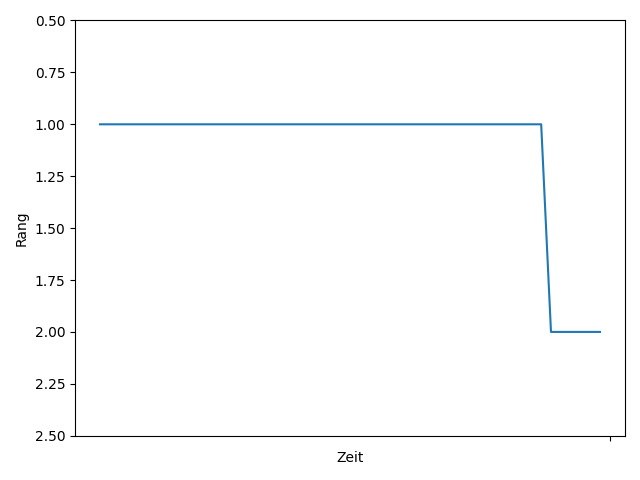
\includegraphics[scale=.25]{JavaTIOBE.png}
    %     \end{subfigure}
    %     \begin{subfigure}[h!]{.5\textwidth}
    %         \caption{Java GitHut 2.0-Index}
    %         \centering
    %         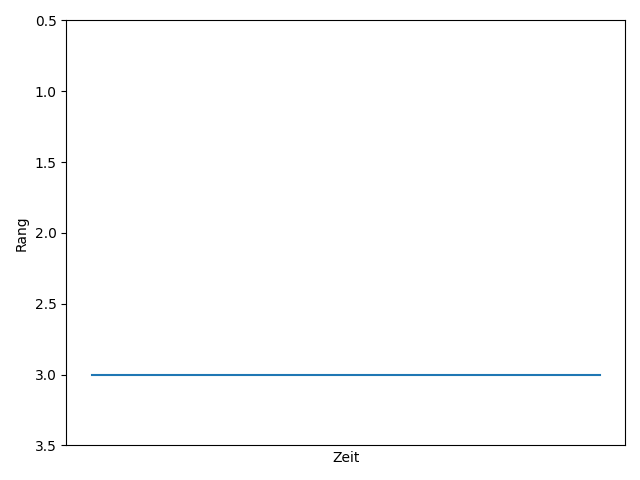
\includegraphics[scale=.25]{JavaGitHut.png}
    %     \end{subfigure}
    % \end{figure}\\
    % Der Verlauf im TIOBE Index deutet an, dass nach Java immer weniger gesucht wird. Das kann daran liegen, dass die Sprache nicht mehr so modern und beliebt ist, oder dass sehr viele Entwickler bereits Java kennen. Auf GitHub ist Java seit dem Quartal 03/2015 auf Platz 3.\\
    % Letztendlich würde ich sagen, dass Java nicht mehr so gefragt ist, wie es mal war. Da jedoch sehr viele Unternehmen noch Java verwenden, und Java bei Android als noch eine große Rolle spielt, wird Java die nächsten Jahre bis Jahrzehnte weiterhin bestehen.\\\\
    % \textbf{Python} wurde von Guido Van Rossum, am "Centrum Wiskunde \& Informatica", im Dezember 1989 angefangen zu Entwickeln. Die erste, öffentliche Version, erschien im Jahr 1991. Python wurde hauptsächlich dafür Entwickelt, eine Programmiersprache zu haben, die Lesbar ist. Die Syntax von Python erlaubt den Entwicklern Konzepte in weniger Codezeilen auszudrücken als mit Java oder C++. \cite{PythonHistory1}\\
    % Python ist eine general purpose Programmiersprache, denn Python wird für so ziemlich alles eingesetzt. Ein Paar verwendungen von Python sind für die Mobile Entwicklung, Spieleentwicklung, Webentwicklung, \nameref{internetofthings} und Datascience. \cite{PythonHistory2}\\
    % Die letzte Version ist Python 3.9, welche am 05. Oktober 2020 veröffentlicht wurde. \cite{PythonLatestRelease} Dies liegt in der 18 Monate Grenze. Daher wird der Verlauf der Beliebtheit auch hier graphisch angegeben:
    % \begin{figure}[h!]
    %     \begin{subfigure}[h!]{.5\textwidth}
    %         \caption{Python TIOBE-Index}
    %         \centering
    %         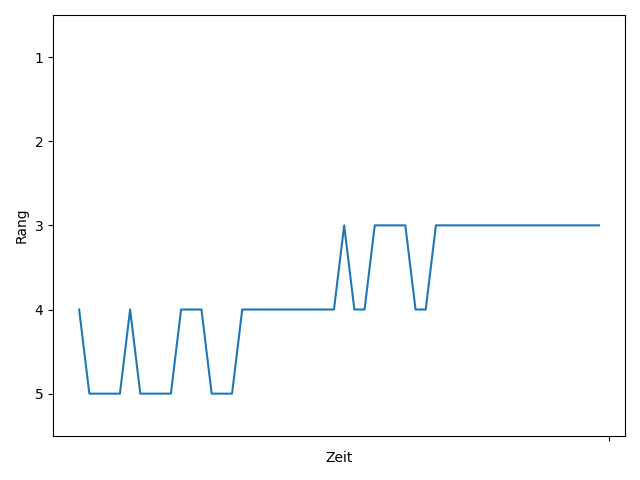
\includegraphics[scale=.25]{PythonTIOBE.png}
    %     \end{subfigure}
    %     \begin{subfigure}[h!]{.5\textwidth}
    %         \caption{Python GitHut 2.0-Index}
    %         \centering
    %         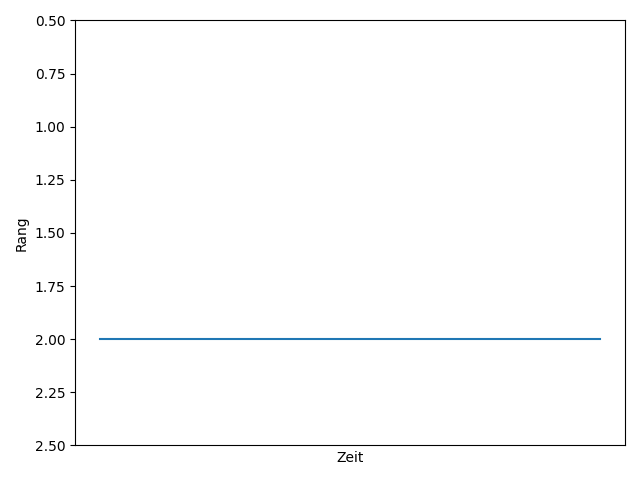
\includegraphics[scale=.25]{PythonGitHut.png}
    %     \end{subfigure}
    % \end{figure}\\
    % Wie bei Java ist auch bei Python die Beliebtheit auf GitHub gleich geblieben, nur dass Python mit Platz 2 beliebter ist als Java.\\
    % Im TIOBE Index hat die beliebtheit am Anfang zwischen Platz 4 und 5 geschwankt, bi dem späteren Verlauf wurde Python jedoch beliebter, bis sie seit einigen Monaten auf Platz 3 liegt. Ein Grund dürfte die, zur Zeit, sehr hohe Nachfrage nach Python sein.\\
    % Da Python immer mehr auf Suchmaschinen gesucht wird und die Beliebtheit bei Pull-Requests auf GitHub die zweithöchste ist, würde ich Python als sehr Zukunftssicher einstufen.\\\\
    % \textbf{C$\sharp$} wurde von Anders Hejlsberg bei Microsoft im Jahr 2000 entwickelt. Die Programmiersprache ist sehr ähnlich zu Java, was daran liegt, dass Microsoft Änderungen an Java vornehmen wollte, Sun es jedoch verboten hat. Das war die Geburtsstunde von C$\sharp$. Sie wurde für die Entwicklung im .NET Framework erstellt und braucht auch die .NET Umgebung um Lauffähig zu sein. Sie ist vor allem sehr gut für die Desktop Entwicklung unter Windows und der Spieleentwicklung geeignet. Jedoch lassen sich mit C$\sharp$ auch Web Anwendungen und Mobile Anwendungen erstellen. \cite{CSharpHistory}\\
    % Die letzte stabile Version von C$\sharp$ ist die Version 8.0, zu welcher von Microsoft am 07. April 2020 ein Beitrag erstellt wurde, was in der Sprache neu ist. \cite{CSharpLatestRelease1}\\
    % Dazu kommt eine Vorschau zu C$\sharp$ 9.0, welche am 20.Mai 2020 veröffentlicht wurde. \cite{CSharpLatestRelease2}\\
    % Da die Vorschauversion keine 18 Monate entfernt veröffentlicht wurde, wird der Beliebtheitsverlauf von C$\sharp$ folgend graphisch dargestellt:
    % \begin{figure}[h!]
    %     \begin{subfigure}[h!]{.5\textwidth}
    %         \caption{C$\sharp$ TIOBE-Index}
    %         \centering
    %         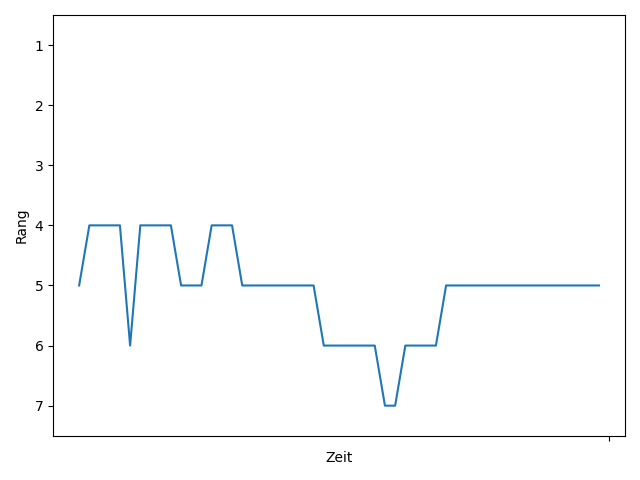
\includegraphics[scale=.25]{CSharpTIOBE.png}
    %     \end{subfigure}
    %     \begin{subfigure}[h!]{.5\textwidth}
    %         \caption{C$\sharp$ GitHut 2.0-Index}
    %         \centering
    %         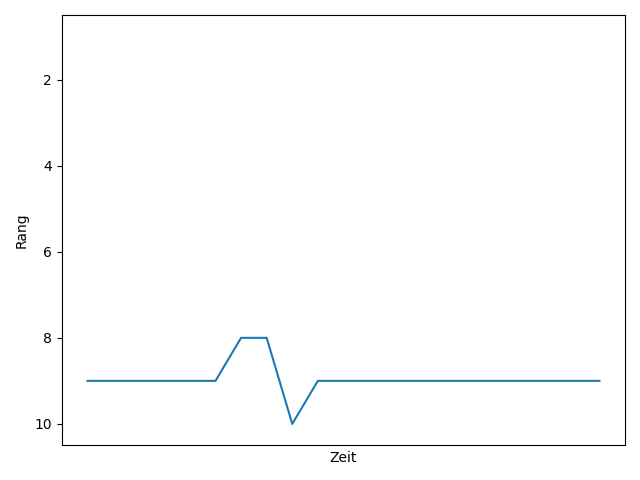
\includegraphics[scale=.25]{CSharpGitHut.png}
    %     \end{subfigure}
    % \end{figure}\newpage\noindent
    % C$\sharp$ ist zwar Syntax-Technisch sehr ähnlich zu Java, jedoch nicht so beliebt. Nach dem TIOBE Index hat C$\sharp$ bis vor wenige Monate einige Schwankungen von den Suchanfragen her. Es ist bis vor wenige Monate ein ständiges Steigen und Fallen, jedoch hält sich C$\sharp$ insgesamt ungefähr auf Platz 5. Anders sieht es auf GitHub aus. Hier sind sehr wenige Schwankungen. Auch hier bleibt insgesamt der Rang von C$\sharp$ ziemlich gleich, auf Platz 9.\\
    % Da C$\sharp$ nicht unbeliebter wird und vor allem sehr viel Verwendung im .NET Framework für die Desktop, Mobile, Web und Spieleentwicklung hat, schätze ich C$\sharp$ als sehr Zukunftssicher ein. Ein Hauptfaktor hierfür ist noch, dass Microsoft, als ein gigantisches Unternehmen, hinter C$\sharp$ steht.\\\\
    % \textbf{Visual Basic .NET} wurde, wie C$\sharp$, von Microsoft entwickelt und 2002 mit dem .NET Framework veröffentlicht. Visual Basic .NET beruht auf Visual Basic, diese können aber nicht miteinander interagieren. Auch mit Visual Basic .NET kann für Windows Dektop, für das Web, Mobile Anwendungen und Office entwickeln. \cite{VBNETHistory}\\
    % Visual Basic .NET scheint zuletzt am 24. Oktober 2018 ein Update erhalten zu haben. \cite{VBNETLatestRelease1}\\
    % Geplant ist die Unterstützung von weiteren Tools in .NET 5, jedoch keine Weiterentwicklung der Programmiersprache selbst. \cite{VBNETLatestRelease2}\\
    % Visual Basic .NET wird nicht mehr weiter betrachtet, da das letzte Update 2 Jahre her ist und die Programmiersprache nicht mehr neue Features bekommt.\\\\
    % \textbf{PHP} wurde 1994 von Rasmus Lerdorf entwickelt. Anfangs war PHP ein Tool, um die Besucherzahlen von seinem online Lebenslauf zu zählen. In Laufe der Zeit hat Rasmus mehr Funktionalitäten hinzugefügt, bis er PHP schließlich neu schrieb. Im Laufe der Zeit erhielt PHP unter anderem eine eingebaute Unterstützung für einige Datenbanksysteme, eigene Funktionen und Cookies. PHP wird Hauptsächlich für die Webentwicklung eingesetzt. \cite{PHPHistory}\\
    % Die letzten Veröffentlichungen von PHP waren am 01. Oktober 2020. \cite{PHPLatestRelease} Damit is PHP in der 18 Monatsgrenze und der Verlauf der Beliebtheit wird auch hier graphisch angezeigt:
    % \begin{figure}[h!]
    %     \begin{subfigure}[h!]{.5\textwidth}
    %         \caption{PHP TIOBE-Index}
    %         \centering
    %         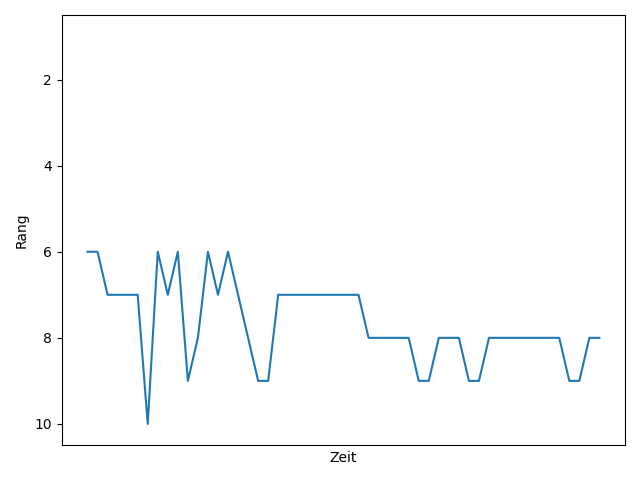
\includegraphics[scale=.25]{PHPTIOBE.png}
    %     \end{subfigure}
    %     \begin{subfigure}[h!]{.5\textwidth}
    %         \caption{PHP GitHut 2.0-Index}
    %         \centering
    %         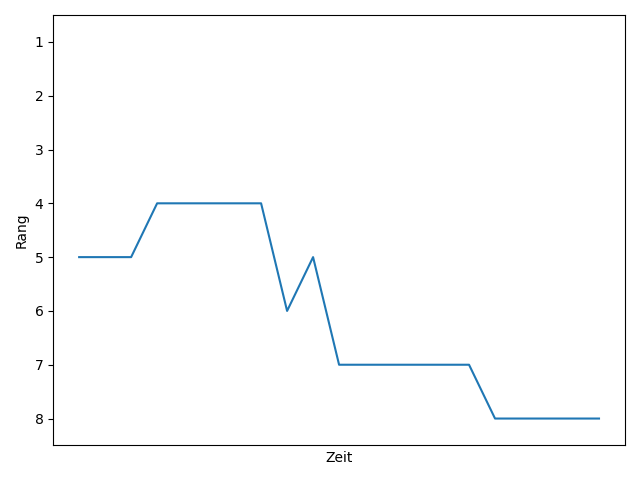
\includegraphics[scale=.25]{PHPGitHut.png}
    %     \end{subfigure}
    % \end{figure}\newpage\noindent
    % Bei PHP gibt es im TIOBE Index anfangs starke Schwankungen der Beliebtheit. Nur sind diese Schwankungen bei PHP stärker. PHP fing an auf Platz 6, und schwankt dann zwischen Platz 6 und 10, bis sie letztendlich zwischen Platz 8 und 9 schwankt. Sichtbar ist hier eine sinkende Tendenz der Beliebtheit.\\
    % Auch auf GitHub kann sich PHP immer weniger auf hohen Plätzen halten. Die Sprache ist erst leicht beliebter geworden, bis sie letztendlich von Platz 5 am Anfang auf Platz 8 im letzten Quartal abgerutscht ist.\\
    % Allerdings wird PHP sehr viel als Backend Sprache auf den Servern eingesetzt.\\
    % Ich stufe PHP nicht als ganz Zukunftssicher ein. Sie wird wahrscheinlich noch sehr lange Zeit Updates erhalten, da scheinbar aber immer weniger Entwickler mit PHP arbeiten wollen, sehe ich keine sehr große Zukunft für PHP.\\\\
    % \textbf{Delhpi/Object Pascal}: Delphi basiert auf Object Pascal. Pascal wurde 1971 von Niklaus Wirth und 1973 entwickelt. Mit Pascal war es möglich, neue Datenstrukturen aus bestehenden zu bilden. Auch wurde dynamische Datenstrukturen unterstützt, so war es möglich Objekte im Laufe des Programms vergrößern oder verkleinern zu können.\\
    % Pascal wurde dafür entwickelt, eine Lehrsprache für Schüler in Programmierklassen zu sein.\\
    % Delphi ist eine Umwandlung von Pascal in eine Objektorientierte Programmiersprache, die auch Datenbankzugriffe erlaubt. \cite{DelphiHistory}\\
    % Die letzte Version von Delphi wurde, laut dem Freepascal Wikipedia, im November 2018 veröffentlich. \cite{DelphiLatestRelease} Daher wird Delhpi/Object Pascal nicht mehr vom Beliebtheitsverlauf betrachtet.\\\\
    % \textbf{Groovy} wurde das erste Mal im Jahr 2003 von James Strachan in seinem Blog erwähnt. Die ersten Veröffentlichungen kamen in den Jahren 2004-2006. Nach einer Versionsumbenennung erschien Groovy 1.0 im Jahr 2007. Leider ist nicht mehr zu der Intention hinter Groovy bekannt, auch in anderen Artikeln. Groovy läuft auf der JVM, wodurch alle Bibliotheken, die unter anderem in Java geschrieben wurden, auch on Groovy verwendet werden können. \cite{GroovyHistory}\\
    % Die letzte Version von Groovy erschien am 26. September 2020 auf dem GitHub Repository. \cite{GroovyLatestRelease} Damit liegt Groovy in der 18 Monate Grenze und der Beliebtheitsverlauf von Groovy wird folgend graphisch angegeben:
    % \begin{figure}[h!]
    %     \begin{subfigure}[h!]{.5\textwidth}
    %         \caption{Groovy TIOBE-Index}
    %         \centering
    %         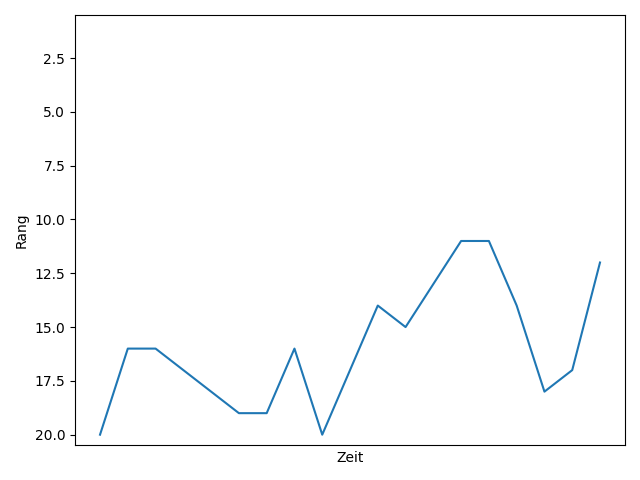
\includegraphics[scale=.25]{GroovyTIOBE.png}
    %     \end{subfigure}
    %     \begin{subfigure}[h!]{.5\textwidth}
    %         \caption{Groovy GitHut 2.0-Index}
    %         \centering
    %         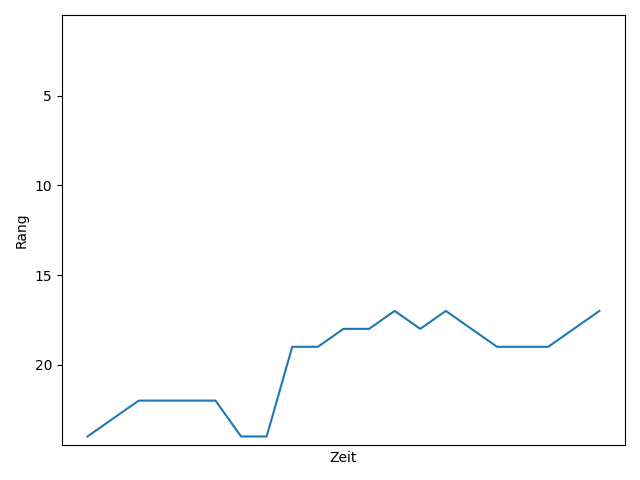
\includegraphics[scale=.25]{GroovyGitHut.png}
    %     \end{subfigure}
    % \end{figure}\\
    % Bei Groovy ist der Trend nicht ganz erkennbar.\\
    % Der TIOBE Index zeigt am Anfang einen Anstieg der Suchen nach Groovy, danach werden die Anfragen jedoch wieder weniger. Später erreicht Groovy seinen Höhepunkt auf Platz 11, jedoch fällt die Nachfrage direkt wieder und steigt dann wieder auf Platz 12.\\
    % Auch auf GitHub steigert Groovy sich vom Platz und fällt wenig später wieder. Dann steigt Groovy wieder, fällt und steigt.\\
    % Ich würde dennoch Groovy als Zukunftssicher einstufen, denn insgesamt wurde die Beliebtheit von Groovy nicht schlechter als sie am Anfang war. Sie steigert sich sogar im Vergleich vor 4-5 Jahren. Nach dem TIOBE Index sind es zwar extreme Unterschiede, jedoch ist der Anstieg auf GitHub stärker als der Fall.\\\\
    % \textbf{Scala} wurde 2001 von Martin Odersky angefangen zu Entwickeln und 2004 veröffentlicht. Da Odersky bei der Entwicklung von Javac (primärer Java Compiler) und Generic Java dabei war, ist Scala ähnlich zu Java. Scala läuft, wie Java und Groovy, ebenfalls auf der JVM. Sie wurde entwickelt, um eine bessere Sprache zu sein. \cite{ScalaHistory}\\
    % Die neueste Version von Scala, 2.12.12, wurde am 13. Juli 2020 veröffentlich. Damit liegt auch Scala in der 18 Monate Grenze. Der Beliebtheitsverlauf wird folgend graphisch dargestellt:
    % \begin{figure}[h!]
    %     \begin{subfigure}[h!]{.5\textwidth}
    %         \caption{Scala TIOBE-Index}
    %         \centering
    %         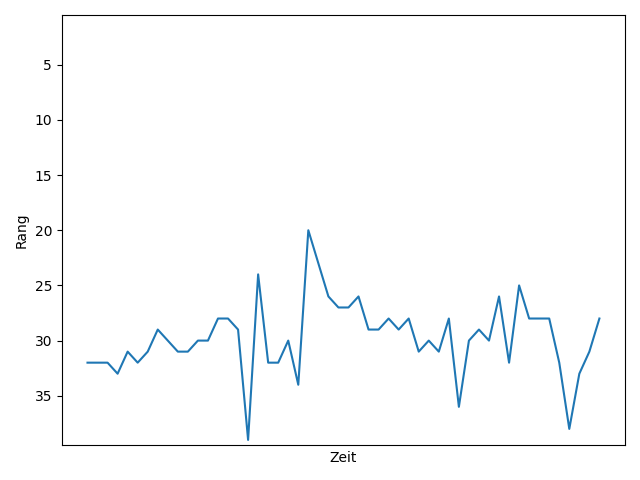
\includegraphics[scale=.25]{ScalaTIOBE.png}
    %     \end{subfigure}
    %     \begin{subfigure}[h!]{.5\textwidth}
    %         \caption{Scala GitHut 2.0-Index}
    %         \centering
    %         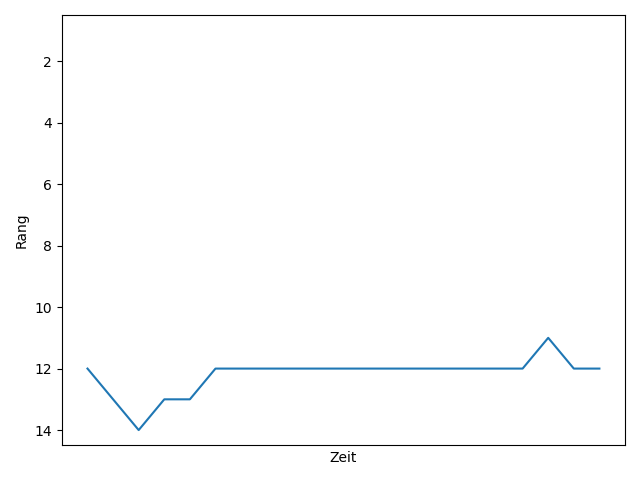
\includegraphics[scale=.25]{ScalaGitHut.png}
    %     \end{subfigure}
    % \end{figure}\newpage\noindent
    % In dem TIOBE Index schwankt der Rang von Scala als hin und her.\\
    % Anfangs wird Scala beliebter von den Suchanfragen her, dann fällt die Beliebtheit. Dann steigt die Beliebtheit noch höher, und fällt direkt wieder. Zurzeit steigt die Beliebtheit wider, wie lange der Anstieg anhält, ist jedoch nicht klar. Nach dem TIOBE Index ist Scala nicht die beliebteste Sprache, jedoch bleibt der Rang auf die Zeit betrachtet ziemlich gleich.\\
    % Scala bewegt sich in dem GitHut Index auf die ganze Zeit gesehen meist auf Platz 12. Es gibt wenige Abweichungen. Damit ist Scala ziemlich stabil von den Pull Requests.\\
    % Ich stufe Scala auch als Zukunftssicher ein. Der Grund ist die hohe Stabilität auf GitHub. Die Suchanfragen nach Scala bringen die Sprache zwar ins Schwanken, aber letztendlich ist Scala auch im TIOBE Index Trendmäßig gleichgeblieben.\\\\
    % \textbf{Kotlin} wurde von Jetbrains 2010 angefangen zu entwickeln. Mit Kotlin kann für Androit, JavaScript, Native und JVM entwickelt werden. Die Programmiersprache ist nicht nur Objektorientiert, sondern auch Funktional. Es werden auch Mischungen erlaubt. Sie wurde entwickelt, um kompakter Programmieren zu können. So lassen sich Programme mit bis zu 40\% weniger Code schreiben. \cite{KotlinHistory}\\
    % Die Letzte Version von Kotlin wurde am 07. September 2020 veröffentlicht. Damit liegt auch Kotlin in der 18 Monate Grenze und der graphische Verlauf der Beliebtheit wird graphisch dargestellt:
    % \begin{figure}[h!]
    %     \begin{subfigure}[h!]{.5\textwidth}
    %         \caption{Kotlin TIOBE-Index}
    %         \centering
    %         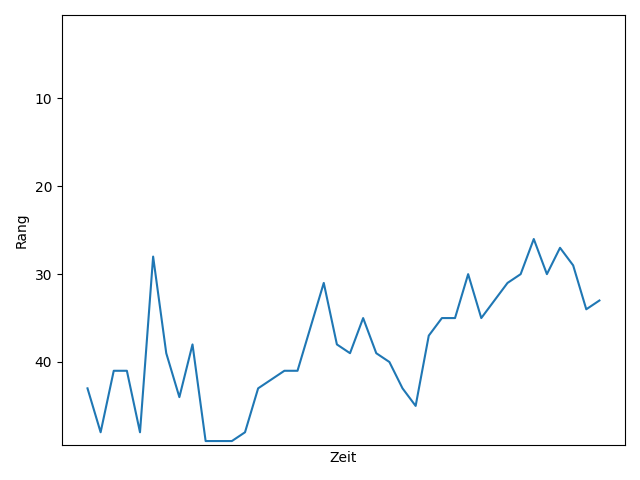
\includegraphics[scale=.25]{KotlinTIOBE.png}
    %     \end{subfigure}
    %     \begin{subfigure}[h!]{.5\textwidth}
    %         \caption{Kotlin GitHut 2.0-Index}
    %         \centering
    %         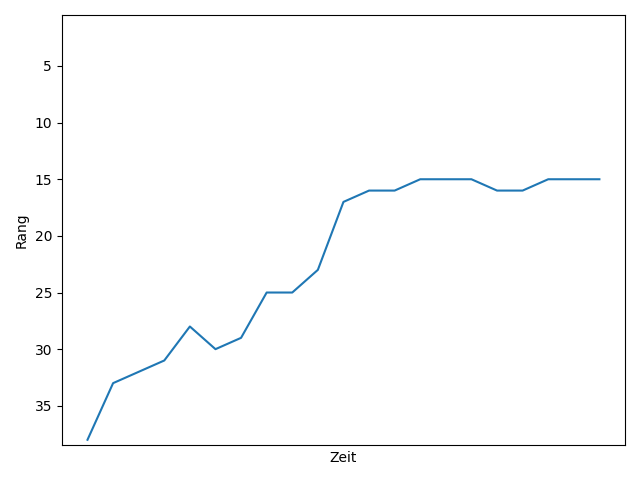
\includegraphics[scale=.25]{KotlinGitHut.png}
    %     \end{subfigure}
    % \end{figure}\newpage\noindent
    % Wie bei Scala ist auch bei Kotlin ein dauerhaftes Schwanken im TIOBE Index.\\
    % Bei Kotlin hingegen ist der Rang letztendlich wesentlich höher als am Anfang.\\
    % Auf GitHub erfreut sich Kotlin immer größerer Beliebtheit. Im Gegensatz zum Anfang hat sich der Rang mehr als verdoppelt und stabilisiert sich letztendlich um den Rang 15.\\
    % Durch den letztendlich höheren Rang im TIOBE Index und den viel höheren Rang im GitHut Index stufe ich Kotlin als Zukunftssicher ein.\\\\
    % Nicht alle Programmiersprachen aus dem ersten Abschnitt wurden als Zukunftssicher eingestuft. Folgende Programmiersprachen werden, da sie als Zukunftssicher eingestuft wurden, für die Ausführungs- und Entwicklungszeiten betrachtet:\\
    % Java, Python, C$\sharp$, Groovy, Scala und Kotlin.
    % \subsubsection{Ausführungsgeschwindigkeit der Programmiersprachen}
    % In diesem Abschnitt werden zuerst allgemeine Performanzvergleiche, wie in \nameref{nonBinaryIntro} beschrieben, herausgesucht.\\
    % Für die "Grobsuche" (Suche nach "Programming language execution performance") werden unter anderem folgende Resultate erhalten:\\
    % Ein Artikel auf Newstack.io beschäftigt sich mit dem Stromverbrauch von 27 verschiedenen Programmiersprachen. Es ist nicht nur der Stromverbrauch, sondern auch der Speicherverbrauch und vor allem die Ausführungszeit von den Programmiersprachen dargestellt. Unter den 27 Programmiersprachen ist Java, C$\sharp$ und Python. Groovy, Scala und Kotlin sind leider nicht mit betrachtet.\\
    % Für den Vergleich in dem Artikel wurden, von 6 Portugisichen Forschern, 10 Probleme von den "Computer Language Benchmarks Game" \cite{Computer Language Benchmarks Game} genommen.\\
    % Nach den Tests zufolge ist, von den übrigen Programmiersprachen aus dem vorherigen Schritt, folgende Reihenfolge der Performanz (Erst genannte Programmiersprachen sind schneller als letzter genannte):\\
    % \begin{enumerate}
    %     \item Java
    %     \item C$\sharp$
    %     \item Python
    % \end{enumerate}
    % \cite{PowerUseage}
    % Dieses Ergebnis ist nicht wirklich verwunderlich, denn Java und C$\sharp$ werden beide in ein Zwischenformat kompiliert und dann ausgeführt, während Python interpretiert wird. Interpretierte Programmiersprachen sind meistens langsamer als kompilierte Programmiersprachen und Programmiersprachen mit einer Zwischenschicht.\\
    % In dem GitHub Repository von attractivechaos wurden verschiedene Algorithmen mit unterschiedlichen Programmiersprachen und Compilern entwickelt. Die Resultate wurden in einer Tabelle dargstellt. \cite{ExecutionPerformance}\\
    % Auf dem ersten Blick ist zu erkennen, dass verschiedene Compiler verschiedene Ausführungsgeschwindigkeiten bei den Programmiersprachen haben.\\\\
    % Überblick über die verschiedenen Compiler:\\
    % \textbf{C$\sharp$}:\\
    % Mono-2.10.1 ist eine Open Source Variante des .NET Frameworks, welches auf Unix, Windows, macOS und anderen Betriebssystemen lauffähig ist. \cite{MonoCSharp}\\
    % \textbf{Java}:\\
    % \texttt{JRE-1.6.0\char`_25} ist das Java Runtime Environment von Oracle, welche Java offiziell verwalten. \cite{JREJava}\\
    % \textbf{Python}:\\
    % PyPy-1.4.1 ist eine JIT Variante von Python, welche meistens schneller läuft, als die standart Python Variante. \cite{PythonPyPy}\\
    % CPython-3.2 und CPython-2.7.1 sind die Interpreter von der offiziellen Python Software Foundation. Die Nummern geben die Version an. \cite{CPython}\\
    % Mono-2.10.1 bietet auch einen Python Interpreter. Durch IronPython ist es möglich Python mit .NET zu verwenden. \cite{IronPython}\\
    % \texttt{JRE-1.6.0\char`_25} erlaubt die Interaktion von Python und Java. Python kann somit von Java ausgeführt und Java von Python ausgeführt werden. \cite{Jython}\\
    % GCC-4.3.2 mit ShedKin-09 ist ein Experiment um Python in C++ umzuwandeln. Es werden allerdings nicht so viele Bibliotheken unterstützt. \cite{ShedSkin}\\\\
    % Für Python wird der CPython Interpreter mit der Version 3.2 betrachtet, da dieser von der Offiziellen Webseite ist und im Vergleich die neuere Version ist.\\\\
    % Nachfolgend werden die 4 auf der GitHub Weiseite betrachteten Programmiersprachen nach der Ausführungszeit und Algorithmus geordnet. A $>$ B bedeutet, dass Programmiersprache A schneller als Programmiersprache B abgeschnitten hat.\\
    % \textbf{sudoku:t}: Java $>$ C$\sharp$ $>$ Python\\
    % \textbf{matmul:t}: Java $>$ C$\sharp$ $>$ Python\\
    % \textbf{matmul:m}: C$\sharp$ $>$ Java $>$ Python\\
    % \textbf{patmch:1t}: Python $>$ Java $>$ C$\sharp$\\
    % \textbf{patmch:2t}: Java $>$ Python $>$ C$\sharp$\\
    % \textbf{dict:t}: Python $>$ C$\sharp$ $>$ Java\\
    % \textbf{dict:m}: C$\sharp$ $>$ Python $>$ Java\\\\
    % Wie zu erkennen ist, sind ist jede der Programmiersprachen mindestens einmal schneller als die anderen 3.\\
    % Da die Ausführungszeit hier unterschiedlich ist und nicht der Ausführungszeitreihenfolge aus der ersten Quelle direkt nachkommt, werde ich eigene Tests schreiben. Diese Tests werden im nächsten Abschnitt genauer beschrieben, nachdem nach bestimmten Bibliotheken gesucht wurde.
    % \subsubsection{Entwicklungszeit der Programmiersprachen}
    % In diesem Abschnitt wird für die Programmiersprachen herausgesucht, ob Bibliotheken für Datenbankverbindungen und INI Dateien einlesen vorhanden sind.\\
    % Als Suchkriterien dienen die Suchen "$<$Programmiersprache$>$ database connection low level" und "$<$Programmiersprache$>$ ini file library".\\
    % Für die Datenbankverbindung werden low level Datenbankbibliotheken bevorzugt, denn diese erlauben den vollen Zugriff auf die Datenbank ohne limitierungen. Außerdem sind diese schneller als Abstraktionen. Anhand dieser Bibliotheken werden dann Performanzvergleiche geführt. Dazu wird eine Datenbank eingerichtet, welche 10.000 Einträge in einer Tabelle enthält. Anschließend wird diese Tabelle ausgelesen und die Datenbankeinträge in einer Liste gespeichert. Weiterhin wird eine INI Datei mit 4 Kategorien und jeweils 5 Einträgen pro Katergorie erstellt. Diese wird eingelesen, jeder Eintrag in einer Liste gespeichert, der letzte Eintrag jeder Kategorie verändert und wieder zurückverändert.\\
    % Die Ausführungsgeschwindigkeit wird mithilfe von der Systemzeit gemessen. Dazu wird die aktuelle Systemzeit vor dem Codeblock gespeichert und diese Zeit von der Systemzeit nach dem Codeblock subtrahiert. Die Programme werden jeweils 50x ausgeführt und der Mittelwert der Ergebnisse genommen.\\
    % Für Entwicklungsgeschwindigkeit wird anhand der notwendigen Codezeilen und dem notwendigen Overhead beurteilt.\\\\
    % Folgende Bibliotheken wurden für die Programmiersprachen gefunden und für den Vergleich genommen:
    % \begin{tabularx}{\textwidth}{|X|X|X|}
    %     \hline
    %     \textbf{Programmiersprache}&\textbf{Datenbank}&\textbf{INI Datei}\\
    %     \hline
    %     \textbf{Java}&JDBC&ini4j\\
    %     \hline
    %     \textbf{Python}&SQLAlchemy&configparser\\
    %     \hline
    %     \textbf{C$\sharp$}&SqlConnection(in System.Data)&ini-parser\\
    %     \hline
    %     \textbf{Groovy}&groovy-sql&ini4j\\
    %     \hline
    %     \textbf{Scala}&JDBC&ini4j\\
    %     \hline
    %     \textbf{Kotlin}&JDBC&ini4j\\
    %     \hline
    % \end{tabularx}
    %%%%%%%%%%%%%%%%%%%%%%%%%%Legende%%%%%%%%%%%%%%%%%%%%%%%%%%
    % \newpage
    % \section{Legende}
    % \fancyhead[R]{Legende}
    % \labelText{\textbf{Computer}}{clientComputer} Hier sind alle möglichen Geräte gemeint, die eine Benutzeroberfläche zur Interaktion haben, auf denen eigene Programme installiert werden können(z.B. PC, Laptop, Smartphone)\\\\
    % \labelText{\textbf{UI}}{nativeApplicationUI} = User Interface. Dies ist die Benutzeroberfläche, also der Teil, mit dem der Nutzer von dem \nameref{clientComputer} interagiert.\\\\
    % \labelText{\textbf{SDK}}{nativeApplicationSDK} = Software Development Kit. Ein SDK ist eine Sammlung von Entwicklungswerkzeugen, wie einen Debugger und Compiler, die die Entwicklung einer Anwendung vereinfachen.\\\\
    % \labelText{\textbf{API}}{crossPlatformAPI} = Application Programming Interface. Eine API wird verwendet, um eine Kommunikation zwischen verschiedenen Software-Anwendungen zu ermöglichen.\\\\
    % \labelText{\textbf{Time Machine}}{timeMachine} Mithilfe der Time Machine lassen sich Webseiten von einem vergangenen Zeitpunk anschauen. Die Time Machine sammelt fast jede aktualisierung einer Webseite, wodurch ein Zugriff auf eine vergange Webseite ermöglicht wird.\\\\
    % \labelText{\textbf{Level}}{programmingLanguageLevel} Das Level einer Programmiersprache gibt an, wie Hardwarenahe diese Programmiersprache ist. Hier wird zwischen "Low Level", "Middle Level" und "High Level" unterschieden. Dabei ist "Low" (z.B. Assembler) sehr Hardwarenahe, "Middle" (z.B. C) abstrakter als "Low" und "High" (z.B. Java) abstrakter als "Middle".
    % \labelText{\textbf{LoC}}{linesOfCode} = Lines of Code. Hiermit sind die Codezeilen eines Programms gemeint, die keine Kommentare sind.\\\\
    % \labelText{\textbf{IoT}}{internetofthings} = Internet of Things. Hierbei kommunizieren Computer mit anderen Maschinen, wobei ein ständiger Datenaustausch stattfindet.\\\\
    % \labelText{\textbf{DOM}}{documentObjectModel} = Document Object Model. Eine Schnittstelle, die XML und HTML Dokumente als Baum betrachtet, in welchem jeder Knoten ein Objekt ist, welches einen Teil des Dokuments darstellt.\\\\
    % \labelText{\textbf{JIT}}{justInTime} = Just in Time. Beim JIT Compiler wird der Code während der Laufzeit kompiliert, anstatt diesen vorher zu kompilieren.
    % References
    \newpage
    \fancyhead[R]{Literatur}
    \begin{thebibliography}{9}
        \bibitem[1]{Native app vs Web app: Multi-criteria decision-making for optimised mobile solution}
        Randleff, Veronica: "Native app vs Web app: Multi-criteria decision-making for optimised mobile solution" (2018): \url{http://kth.diva-portal.org/smash/record.jsf?pid=diva2%3A1231519&dswid=-9092}
        \bibitem[2]{Extending browser platforms with native capabilities}
        Nicklas, Schultz: "Extending browser platforms with native capabilities, enabling additional features in a media streaming context" (2015): \url{http://liu.diva-portal.org/smash/record.jsf?pid=diva2%3A828065&dswid=-8186}
        \bibitem[3]{Cross-platform development of smartphone applications: An evaluation of React Native}
        Furuskog, Martin; Wemyss, Stuart: "Cross-platform development of smartphone applications: An evaluation of React Native" (2016): \url{http://uu.diva-portal.org/smash/record.jsf?pid=diva2%3A948617&dswid=7703}
        \bibitem[NAD]{Native Application Development}
        Native Entwicklung: \url{https://searchsoftwarequality.techtarget.com/definition/native-application-native-app} (23.10.2020)
        \bibitem[BNA]{NativeAdvantages}
        Vorteile nativer Anwendungen\url{https://mlsdev.com/blog/native-app-development-vs-web-and-hybrid-app-development} (26.10.2020)
        \bibitem[DANA]{NativeDisadvantages}
        Vor- und Nachteile einer Nativen, Web und Hybriden Anwendung\url{https://threefourteen.ie/blog/advantages-and-disadvantages-of-web-native-and-hybrid-apps/} (26.10.2020)
        \bibitem[CPD]{CrossPlatform}
        Cross-Platform Definition: \url{https://www.techopedia.com/definition/30026/cross-platform-development} (26.10.2020)
        \bibitem[CPDA]{CrossPlatformA}
        Cross-Platform Vorteile: \url{https://medium.com/successivetech/benefits-of-cross-platform-development-bfa5f708c0a4} (26.10.2020)
        \bibitem[CPDD]{CrossPlatformD}
        Cross-Platform Vorteile: \url{https://www.focaloid.com/blog/the-pros-and-cons-of-cross-platform-apps} (26.10.2020)
        \bibitem[CPDDA]{CrossPlatformAD}
        Cross-Platform Vor- und Nachteile: \url{https://codeburst.io/native-vs-cross-platform-app-development-pros-and-cons-49f397bb38ac} (26.10.2020)
        \bibitem[WDD]{WebDevelopment2}
        Web Entwicklung Definition: \url{https://www.techopedia.com/definition/23889/web-development} (01.10.2020)
        \bibitem[WDF]{WebDevelopment}
        Web Entwicklung Funktionsweise: \url{https://networkencyclopedia.com/web-application/} (01.10.2020)
        \bibitem[BWD]{AdvantagesWebDevelopment}
        Vorteile Web Entwicklung: \url{https://www.nirvanacanada.com/businessonline/the-benefits-of-web-application-development-for-businesses/} (01.10.2020)
        \bibitem[ADWD]{ADWebDevelopment}
        Vor- und Nachteile Web Entwicklung: \url{https://en.yeeply.com/blog/advantages-and-disadvantages-of-web-app-development/} (06.10.2020)
        \bibitem[DWD]{DisadvantagesWebDevelopment}
        Nachteile Web Entwicklung: \url{https://www.linkedin.com/pulse/advantages-disadvantages-web-app-development-luis-picurelli} (01.10.2020)
        \bibitem[HD]{HybrideDevelopment}
        Vorteile Web Entwicklung: \url{https://clearbridgemobile.com/mobile-app-development-native-vs-web-vs-hybrid/} (06.10.2020)
        \bibitem[TI]{TIOBE Index}
        TIOBE Index Beschreibung (über erste Tabelle): \url{https://www.tiobe.com/tiobe-index/} (30.10.2020)
        \bibitem[GH2.0]{GitHut 2.0}
        GitHut 2.0 Beschreibung (unter PI-Chart): \url{https://madnight.github.io/githut/#/pull_requests/2020/3} (30.10.2020)
        \bibitem[HLLL]{High level Low level languages}
        "Hochsprachen" und "Tiefsprachen": \url{https://careerkarma.com/blog/high-level-and-low-level-languages/} (30.10.2020)
        \bibitem[TI1219]{TIOBE Index 12.2019}
        TIOBE Index von Dezember 2019: \url{https://web.archive.org/web/20191231193250/https://www.tiobe.com/tiobe-index/} (30.10.2020)
        \bibitem[TI0120]{TIOBE Index 01.2020}
        TIOBE Index von Januar 2020: \url{https://web.archive.org/web/20200131222240/https://www.tiobe.com/tiobe-index/} (30.10.2020)
        \bibitem[TI0220]{TIOBE Index 02.2020}
        TIOBE Index von Februar 2020: \url{https://web.archive.org/web/20200229165403/https://www.tiobe.com/tiobe-index/} (30.10.2020)
        \bibitem[TI0320]{TIOBE Index 03.2020}
        TIOBE Index von März 2020: \url{https://web.archive.org/web/20200328111140/https://www.tiobe.com/tiobe-index/} (30.10.2020)
        \bibitem[TI0420]{TIOBE Index 04.2020}
        TIOBE Index von April 2020: \url{https://web.archive.org/web/20200430164914/https://www.tiobe.com/tiobe-index/} (30.10.2020)
        \bibitem[TI0520]{TIOBE Index 05.2020}
        TIOBE Index von Mai 2020: \url{https://web.archive.org/web/20200531144216/https://www.tiobe.com/tiobe-index/} (30.10.2020)
        \bibitem[TI0620]{TIOBE Index 06.2020}
        TIOBE Index von Juni 2020: \url{https://web.archive.org/web/20200627171928/https://www.tiobe.com/tiobe-index/} (30.10.2020)
        \bibitem[TI0720]{TIOBE Index 07.2020}
        TIOBE Index von Juli 2020: \url{https://web.archive.org/web/20200731064026/https://www.tiobe.com/tiobe-index/} (30.10.2020)
        \bibitem[TI0820]{TIOBE Index 08.2020}
        TIOBE Index von August 2020: \url{https://web.archive.org/web/20200831103505/https://www.tiobe.com/tiobe-index/} (30.10.2020)
        \bibitem[TI0920]{TIOBE Index 09.2020}
        TIOBE Index von September 2020: \url{https://web.archive.org/web/20200929231011/https://www.tiobe.com/tiobe-index/} (30.10.2020)
        \bibitem[TI1020]{TIOBE Index 10.2020}
        TIOBE Index von Oktober 2020: \url{https://web.archive.org/web/20201028100442/https://www.tiobe.com/tiobe-index/} (30.10.2020)
        \bibitem[GH419]{GitHut 2.0 4/2019}
        GitHut 2.0 vom Quartal 4/2019: \url{https://madnight.github.io/githut/#/pull_requests/2019/4} (31.10.2020)
        \bibitem[GH120]{GitHut 2.0 1/2020}
        GitHut 2.0 vom Quartal 1/2020: \url{https://madnight.github.io/githut/#/pull_requests/2020/1} (31.10.2020)
        \bibitem[GH220]{GitHut 2.0 2/2020}
        GitHut 2.0 vom Quartal 2/2020: \url{https://madnight.github.io/githut/#/pull_requests/2020/2} (31.10.2020)
        \bibitem[GH320]{GitHut 2.0 3/2020}
        GitHut 2.0 vom Quartal 3/2020: \url{https://madnight.github.io/githut/#/pull_requests/2020/3} (31.10.2020)
        \bibitem[JL1]{JavaLevel1}
        Java Sprachlevel Oracle: \url{https://docs.oracle.com/javase/specs/jls/se8/html/jls-1.html} (01.11.2020)
        \bibitem[JL2]{JavaLevel2}
        Java Sprachlevel Medium: \url{https://medium.com/@escalesolutions/java-tutorial-best-five-tutorials-to-master-java-programming-language-in-2018-9916987df48} (01.11.2020)
        \bibitem[CL1]{CLevel1}
        C Sprachlevel Course Report: \url{https://www.coursereport.com/blog/a-guide-to-low-level-programming-for-beginners} (01.11.2020)
        \bibitem[CL2]{CLevel2}
        C Sprachlevel Medium: \url{https://medium.com/swlh/a-high-level-introduction-to-the-c-programming-language-f5ada5a5bd5d} (01.11.2020)
        \bibitem[C++L]{C++Level1}
        C++ Sprachlevel GeeksForGeeks: \url{https://www.geeksforgeeks.org/introduction-to-c-programming-language/} (01.11.2020)
        \bibitem[PL1]{PythonLevel1}
        Python Sprachlevel Python: \url{https://www.python.org/doc/essays/blurb/} (01.11.2020)
        \bibitem[PL2]{PythonLevel2}
        Python Sprachlevel hackr.io: \url{https://hackr.io/blog/python-programming-language} (01.11.2020)
        \bibitem[C$\sharp$L1]{CSLevel1}
        C$\sharp$ Sprachlevel Medium: \url{https://medium.com/sololearn/why-is-c-among-the-most-popular-programming-languages-in-the-world-ccf26824ffcb} (01.11.2020)
        \bibitem[C$\sharp$L2]{CSLevel2}
        C$\sharp$ Sprachlevel Cateer Karma: \url{https://careerkarma.com/blog/c-plus-plus-vs-c-sharp/} (01.11.2020)
        \bibitem[VBNETL1]{VBNLevel1}
        Visual Basic .NET Sprachlevel Researchgate: \url{https://www.researchgate.net/publication/267788607_CIL_Programming_Under_the_Hood_of_NET} (01.11.2020)
        \bibitem[VBNETL2]{VBNLevel2}
        Visual Basic .NET Sprachlevel Acseduonline: \url{https://www.acseduonline.com/courses/information-technology-computers-5/visual-basic-net-bit101-442.aspx} (01.11.2020)
        \bibitem[JSL1]{JSL1}
        JavaScript Sprachlevel PluralsightPluralsight: \url{https://www.pluralsight.com/paths/javascript-core-language} (01.11.2020)
        \bibitem[JSL2]{JSL2}
        JavaScript Sprachlevel Tutsplus: \url{https://code.tutsplus.com/tutorials/what-is-javascript--cms-26177} (01.11.2020)
        \bibitem[PHPL]{PHPLevel}
        PHP Sprachlevel EDUCBA: \url{https://www.educba.com/high-level-languages-vs-low-level-languages/} (02.11.2020)
        \bibitem[SQLL]{SQLLevel}
        SQL Sprachlevel Oracle Patches: \url{https://oracle-patches.com/en/databases/sql/4191-sql-programming-language-and-oracle-novations} (02.11.2020)
        \bibitem[SWL1]{SwiftLevel1}
        Swift Sprachlevel bestprogramminglanguagefor.me: \url{https://www.bestprogramminglanguagefor.me/why-learn-swift} (02.11.2020)
        \bibitem[SWL2]{SwiftLevel2}
        Swift Sprachlevel Infoq: \url{https://www.infoq.com/news/2014/06/apple-swift/} (02.11.2020)
        \bibitem[RL1]{RubyLevel1}
        Ruby Sprachlevel bestprogramminglanguagefor.me: \url{https://www.bestprogramminglanguagefor.me/why-learn-ruby} (02.11.2020)
        \bibitem[RL2]{RubyLevel2}
        Ruby Sprachlevel isleofruby: \url{http://isleofruby.org/learn-ruby-over-other-programming-languages/} (02.11.2020)
        \bibitem[DL2]{DelphiLevel1}
        Delphi/Object Pascal Sprachlevel isleofruby: \url{http://docwiki.embarcadero.com/RADStudio/Sydney/en/Language_Overview} (02.11.2020)
        \bibitem[DL2]{DelphiLevel2}
        Delphi/Object Pascal Sprachlevel isleofruby: \url{https://kolmck.net/general-information-delphi-programming-language/} (02.11.2020)
        \bibitem[OCL]{ObjCLevel}
        Objective-C Sprachlevel gsdh: \url{https://www.gsdh.org/en/objectivec.html} (02.11.2020)
        \bibitem[ASL1]{AssLanLevel1}
        Assembly Language Sprachlevel isleofruby: \url{https://www.tutorialspoint.com/assembly_programming/index.htm} (02.11.2020)
        \bibitem[ASL2]{AssLanLevel2}
        Assembly Language Sprachlevel gsdh: \url{https://www.educba.com/what-is-assembly-language/} (02.11.2020)
        \bibitem[GL]{GoLevel}
        Go Sprachlevel Medium: \url{https://medium.com/@imdanielsp/go-programming-language-analysis-i-989eab66a34a} (02.11.2020)
        \bibitem[RL]{RLevel}
        R Sprachlevel Codementor: \url{https://www.codementor.io/@sayantinideb/r-vs-python-best-programming-language-for-data-science-and-analysis-te05xgx98} (03.11.2020)
        \bibitem[MLL]{MATLABLevel}
        MATLAB Sprachlevel Springerprofessional: \url{https://www.springerprofessional.de/en/matlab-programming-for-numerical-analysis/1903816} (03.11.2020)
        \bibitem[MLL]{DLevel1}
        D Sprachlevel Dlang: \url{https://dlang.org/overview.html} (03.11.2020)
        \bibitem[MLL]{DLevel2}
        D Sprachlevel Computerhope: \url{https://www.computerhope.com/jargon/d/dlang.htm} (03.11.2020)
        \bibitem[VBL]{PerlLevel1}
        Perl Sprachlevel Perl Dokumentation: \url{https://perldoc.perl.org/perlfaq1} (03.11.2020)
        \bibitem[VBL]{PerlLevel2}
        Perl Sprachlevel GeeksForGeeks: \url{https://www.geeksforgeeks.org/perl-programming-language/} (03.11.2020)
        \bibitem[RL]{RustLevel}
        Rust Sprachlevel dev.to: \url{https://dev.to/lambdude/comment/1okc} (03.11.2020)
        \bibitem[GL]{GroovyLevel}
        Groovy Sprachlevel cs.com: \url{https://wiki.c2.com/?GroovyLanguage} (03.11.2020)
        \bibitem[DTL1]{DartLevel1}
        Dart Sprachlevel codecarbon: \url{https://codecarbon.com/pros-cons-dart-language/} (03.11.2020)
        \bibitem[DTL2]{DartLevel2}
        Dart Sprachlevel javatpoint: \url{https://www.javatpoint.com/dart-programming} (03.11.2020)
        \bibitem[TS]{TypeScript}
        Typescript offizielle Webseite: \url{https://www.typescriptlang.org/} (03.11.2020)
        \bibitem[SCL1]{ScalaLevel1}
        Scala Sprachlevel offizielle Webseite: \url{https://www.scala-lang.org/} (03.11.2020)
        \bibitem[SCL2]{ScalaLevel2}
        Scala Sprachlevel Toptal: \url{https://www.toptal.com/scala/why-should-i-learn-scala} (03.11.2020)
        \bibitem[KL]{KotlinLanguage}
        Kotlin offizielle Webseite: \url{https://kotlinlang.org/} (03.11.2020)
        \bibitem[LL]{LuaLevel}
        Lua Sprachlevel Medium: \url{https://medium.com/turing-ninjas/the-double-edged-programming-language-lua-easy-for-kids-to-learn-and-also-powerful-enough-for-ca772e24a32b} (03.11.2020)
        \bibitem[Vaadin]{JavaVaadin}
        Java Vaadin Framework: \url{https://vaadin.com/} (04.11.2020)
        \bibitem[Anvil]{PythonAnvil}
        Python Anvil Framework: \url{https://anvil.works/} (04.11.2020)
        \bibitem[Radzen]{CSharpRadzen}
        C$\sharp$ Radzen (Blazor) Framework: \url{https://www.radzen.com/blog/build-web-applications-with-radzen-blazor-csharp-no-javascript-required/} (04.11.2020)
        \bibitem[WF1]{WebForms1}
        Artikel über WebForms: \url{https://docs.microsoft.com/en-us/archive/msdn-magazine/2001/may/asp-net-web-forms-let-you-drag-and-drop-your-way-to-powerful-web-apps} (05.11.2020)
        \bibitem[WF2]{WebForms2}
        WebForms Webseite: \url{https://dotnet.microsoft.com/apps/aspnet/web-forms} (05.11.2020)
        \bibitem[WX]{Webix}
        Webix Webseite: \url{https://webix.com/} (06.11.2020)
        \bibitem[IP]{impresspages}
        Impresspages: \url{https://www.impresspages.org/} (06.11.2020)
        \bibitem[RS]{raudus}
        Raudus Webseite: \url{https://www.raudus.com/} (07.11.2020)
        \bibitem[TSW]{TSWebix}
        TypeScript Webix: \url{https://blog.webix.com/typescript-types-in-webix-ui-framework/} (08.11.2020)
        \bibitem[SV]{ScalaVaadin}
        Scala Vaadin: \url{https://vaadin.com/docs/v8/framework/getting-started/getting-started-scala.html} (08.11.2020)
        \bibitem[KV]{KotlinVaadin}
        Kotlin Vaadin: \url{https://vaadin.com/kotlin} (08.11.2020)
        \bibitem[JH]{JavaHistory}
        Java Gründung: \url{https://www.javatpoint.com/history-of-java} (11.11.2020)
        \bibitem[JLR]{JavaLatestRelease}
        Java letztes Update: \url{https://www.codejava.net/java-se/java-se-versions-history} (11.11.2020)
        \bibitem[PH1]{PythonHistory1}
        Python Gründung Teil 1: \url{https://www.geeksforgeeks.org/history-of-python/} (12.11.2020)
        \bibitem[PH2]{PythonHistory2}
        Python Gründung Teil 2: \url{https://www.javatpoint.com/python-history} (12.11.2020)
        \bibitem[PLR]{PythonLatestRelease}
        Python letztes Update: \url{https://www.python.org/downloads/} (12.11.2020)
        \bibitem[CSH]{CSharpHistory}
        C$\sharp$ Gründung: \url{https://medium.com/sololearn/why-is-c-among-the-most-popular-programming-languages-in-the-world-ccf26824ffcb} (12.11.2020)
        \bibitem[CSLR1]{CSharpLatestRelease1}
        C$\sharp$ letztes Update 8.0: \url{https://docs.microsoft.com/en-us/dotnet/csharp/whats-new/csharp-8} (12.11.2020)
        \bibitem[CSLR2]{CSharpLatestRelease2}
        C$\sharp$ letztes Update 9.0: \url{https://devblogs.microsoft.com/dotnet/welcome-to-c-9-0/} (12.11.2020)
        \bibitem[VBNETH]{VBNETHistory}
        Visual Basic .NET Gründung: \url{https://www.guru99.com/vb-net-introduction-features.html} (12.11.2020)
        \bibitem[VBNETLR1]{VBNETLatestRelease1}
        Visual Basic .NET letztes Update 16.0: \url{https://docs.microsoft.com/en-us/dotnet/visual-basic/whats-new/#visual-basic-160} (12.11.2020)
        \bibitem[VBNETLR2]{VBNETLatestRelease2}
        Visual Basic .NET weiteres Update: \url{https://devblogs.microsoft.com/vbteam/visual-basic-support-planned-for-net-5-0/} (12.11.2020)
        \bibitem[JSH]{JavaScriptHistory}
        JavaScript Gründung: \url{https://careerkarma.com/blog/javascript-history/} (13.11.2020)
        \bibitem[JSLR]{JavaScriptLatestRelease}
        JavaScript letztes Update: \url{https://www.freecodecamp.org/news/javascript-new-features-es2020/} (13.11.2020)
        \bibitem[PHPH]{PHPHistory}
        PHP Gründung: \url{https://www.php.net/manual/en/history.php.php} (13.11.2020)
        \bibitem[PHPLR]{PHPLatestRelease}
        PHP letzte Veröffentlichung: \url{https://www.php.net/releases/index.php} (13.11.2020)
        \bibitem[DH]{DelphiHistory}
        Delphi/Object Pascal Gründung: \url{https://vakrio.medium.com/history-of-delphi-from-pascal-to-embarcadero-delphi-xe-2-c6809366ae45} (13.11.2020)
        \bibitem[DLR]{DelphiLatestRelease}
        Delphi/Object Pascal letzte Veröffentlichung: \url{https://wiki.freepascal.org/Delphi} (13.11.2020)
        \bibitem[GH]{GroovyHistory}
        Groovy Gründung: \url{https://www.cleverism.com/skills-and-tools/groovy/} (13.11.2020)
        \bibitem[GLR]{GroovyLatestRelease}
        Groovy letztes Update: \url{https://github.com/apache/groovy/releases} (13.11.2020)
        \bibitem[TSH]{TypeScriptHistory}
        TypeScript Gründung: \url{https://coderlipi.com/typescript/typescript-history} (15.11.2020)
        \bibitem[TSLR]{TypeScriptLatestRelease}
        TypeScript letztes Update: \url{https://github.com/microsoft/TypeScript/releases} (15.11.2020)
        \bibitem[SH]{ScalaHistory}
        Scala Gründung: \url{https://www.educative.io/courses/learn-scala-from-scratch/39BnN6DMZxr} (16.11.2020)
        \bibitem[SLR]{ScalaLatestRelease}
        Scala letztes Update: \url{https://github.com/scala/scala/releases} (16.11.2020)
        \bibitem[SH]{KotlinHistory}
        Kotlin Gründung: \url{https://kotlinlang.org/docs/reference/faq.html} (16.11.2020)
        \bibitem[SLR]{KotlinLatestRelease}
        Kotlin letztes Update: \url{https://kotlinlang.org/releases.html} (16.11.2020)
        \bibitem[CLBG]{Computer Language Benchmarks Game}
        Computer Language Benchmarks Game: \url{https://en.wikipedia.org/wiki/The_Computer_Language_Benchmarks_Game} (17.11.2020)
        \bibitem[PU]{PowerUseage}
        Stromvergleich von Thenewstack.io: \url{https://thenewstack.io/which-programming-languages-use-the-least-electricity/} (19.11.2020)
        \bibitem[EP]{ExecutionPerformance}
        Aufsührungszeit vergleich von attractivechaos: \url{https://attractivechaos.github.io/plb/} (20.11.2020)
        \bibitem[MCS]{MonoCSharp}
        Mono-2.10.1: \url{https://www.mono-project.com/docs/about-mono/releases/2.10.1/} (20.11.2020)
        \bibitem[JREJ]{JREJava}
        \texttt{JRE-1.6.0\char`_25}: \url{https://blogs.oracle.com/ebstech/sun-jre-16025-certified-with-oracle-e-business-suite} (20.11.2020)
        \bibitem[V8JS]{JavaScriptV8}
        V8-r8384: \url{https://v8.dev/} (20.11.2020)
        \bibitem[JMJS]{JavaScriptJaegerMonkey}
        JaegarMonkey-a95d42642281: \url{https://wiki.mozilla.org/JaegerMonkey} (20.11.2020)
        \bibitem[PPP]{PythonPyPy}
        PyPy: \url{https://www.pypy.org/} (20.11.2020)
        \bibitem[CP]{CPython}
        CPython: \url{https://github.com/python/cpython} (20.11.2020)
        \bibitem[IP]{IronPython}
        IronPython: \url{https://ironpython.net/} (20.11.2020)
        \bibitem[J]{Jython}
        Jython: \url{https://www.jython.org/} (20.11.2020)
        \bibitem[SS]{ShedSkin}
        ShedSkin: \url{https://github.com/shedskin/shedskin} (20.11.2020)
        \bibitem[TD]{TIOBEDefinition}
        TIOBE Definition: \url{https://www.tiobe.com/tiobe-index/programming-languages-definition/} (29.11.2020)
        \bibitem[JWF1]{JavaWebFramework1}
        Mehrere Java Frameworks Vorstellung: \url{https://hackr.io/blog/java-frameworks} (14.12.2020)
        \bibitem[JVD]{JavaVaadinDesigner}
        Vaadin Designer: \url{https://vaadin.com/designer} (14.12.2020)
        \bibitem[JJC]{JavaJudo}
        Judo.codes: \url{https://www.judo.codes/features} (15.12.2020)
        \bibitem[JOSBP]{JavaOSBP}
        Eclipse OSBP: \url{https://www.eclipse.org/osbp/index.html} (15.12.2020)
        \bibitem[OEP]{OEP Main Page}
        Opcenter Execution Pharma Hauptseite: \url{https://www.plm.automation.siemens.com/global/de/products/manufacturing-operations-center/simatic-it-ebr.html} (21.12.2020)
        \bibitem[KKV]{Kotlin KVision}
        KVision GitHub Seite: \url{https://github.com/rjaros/kvision} (29.12.2020)
        \bibitem[KCO]{Kotlin Codename One}
        Codename One: \url{https://www.codenameone.com/} (29.12.2020)
        \bibitem[PWB]{Python Webbot}
        Webbot Webseite: \url{http://www.webbot.ws/Home} (31.12.2020)
        \bibitem[PW]{Python Widgy}
        Widgy Webseite: \url{https://wid.gy/} (31.12.2020)
        \bibitem[CSW]{CSharp Wisej}
        Wisey: \url{https://wisej.com/} (31.12.2020)
        \bibitem[JD]{JSFDeveloper}
        JSF Entwickler: \url{https://www.oracle.com/java/technologies/javaserverfaces.html} (02.01.2021)
        \bibitem[JLA]{JSFLatestUpdate}
        JSF Entwickler: \url{https://jcp.org/en/jsr/detail?id=372} (02.01.2021)
        \bibitem[JC]{JSFCompaniesUsing}
        Unternehmen, die JSF nutzen: \url{https://www.wappalyzer.com/technologies/web-frameworks/javaserver-faces/} (02.01.2021)
        \bibitem[VD]{VaadinDeveloper}
        Vaadin Entwickler: \url{https://vaadin.com/} (02.01.2021)
        \bibitem[VLA]{VaadinReleases}
        Vaadin letzte Updates: \url{https://vaadin.com/releases} (02.01.2021)
        \bibitem[VC]{VaadinCompanies}
        Unternehmen, die Vaadin nutzen: \url{https://medium.com/javarevisited/top-companies-brands-using-vaadin-framework-5360d0cc09b9} (02.01.2021)
        \bibitem[KVD]{KVisionDeveloper}
        KVision Entwickler: \url{https://github.com/rjaros} (02.01.2021)
        \bibitem[KVLA]{KVisionReleases}
        KVision letzte Updates: \url{https://github.com/rjaros/kvision/releases} (02.01.2021)
        \bibitem[COD]{CodenameOneDeveloper}
        Codename One Entwickler: \url{https://www.codenameone.com/about-us.html} (02.01.2021)
        \bibitem[COLA1]{CodenameOneReleases1}
        Codename One letzte Updates 1: \url{https://plugins.jetbrains.com/plugin/7357-codename-one/versions} (02.01.2021)
        \bibitem[COLA2]{CodenameOneReleases2}
        Codename One letzte Updates 2: \url{http://plugins.netbeans.org/plugin/42406/codename-one} (02.01.2021)
        \bibitem[COC]{CodenameOneCompanies}
        Unternehmen, die Codename One nutzen: \url{https://enlyft.com/tech/products/codename-one} (02.01.2021)
        \bibitem[WBD]{WebBotDeveloper}
        WebBot Entwickler: \url{https://pypi.org/project/webbot/} (02.01.2021)
        \bibitem[WBLA]{WebBotReleases}
        WebBot letzte Updates: \url{https://pypi.org/project/webbot/#files} (02.01.2021)
        \bibitem[WBD]{AnvilDeveloper}
        Anvil Entwickler: \url{https://anvil.works/about-us} (02.01.2021)
        \bibitem[WBLA]{AnvilReleases}
        Anvil letzte Updates: \url{https://github.com/anvil-works/anvil-runtime} (02.01.2021)
        \bibitem[WBC]{AnvilCompanies}
        Unternehmen, die Anvil nutzen: \url{https://anvil.works/} (02.01.2021)
        \bibitem[DD]{DjangoDeveloper}
        Django Entwickler: \url{https://www.djangoproject.com/foundation/} (02.01.2021)
        \bibitem[WD]{WidgyDeveloper}
        Widgy Entwickler: \url{https://wid.gy/} (02.01.2021)
        \bibitem[DLA]{DjangoReleases}
        Django letzte Updates: \url{https://pypi.org/project/Django/#history} (02.01.2021)
        \bibitem[WLA]{WidgyReleases}
        Widgy letzte Updates: \url{https://pypi.org/project/django-widgy/} (02.01.2021)
        \bibitem[WBC]{DjangoCompanies}
        Unternehmen, die Django nutzen: \url{https://medium.com/@thakuramit92/8-popular-companies-use-django-for-their-web-applications-531cdd21ac38} (02.01.2021)
        \bibitem[WD]{WisejDeveloper}
        Wisej Entwickler: \url{https://wisej.com/contact/} (02.01.2021)
        \bibitem[WLA]{WisejReleases}
        Wisej letzte Updates: \url{https://wisej.com/builds/} (02.01.2021)
        \bibitem[WC]{WisejCompanies}
        Unternehmen, die Wisej nutzen: \url{https://madewithwisej.com/page/3/} (02.01.2021)
        \bibitem[WFD]{WebFormsDeveloper}
        WebForms Entwickler: \url{https://docs.microsoft.com/en-us/aspnet/web-forms/what-is-web-forms} (02.01.2021)
        \bibitem[WFLA]{WebFormsReleases}
        WebForms letzte Updates: \url{https://docs.microsoft.com/en-us/aspnet/web-forms/overview/getting-started/getting-started-with-aspnet-45-web-forms/} (02.01.2021)
        \bibitem[RD]{RadzenDeveloper}
        Radzen Entwickler: \url{https://www.radzen.com/about/} (03.01.2021)
        \bibitem[RLA]{RadzenReleases}
        Radzen letzte Updates: \url{https://www.radzen.com/documentation/changelog/} (03.01.2021)
        \bibitem[RC]{RadzenCompanies}
        Unternehmen, die Radzen nutzen: \url{https://www.radzen.com/} (03.01.2021)
        \bibitem[BD]{BlazorDeveloper}
        Blazor Entwickler: \url{https://dotnet.microsoft.com/apps/aspnet/web-apps/blazor} (03.01.2021)
        \bibitem[BLA]{BlazorReleases}
        Blazor letzte Updates: \url{https://github.com/dotnet/blazor/releases} (03.01.2021)
        \bibitem[BC]{BlazorCompanies}
        Unternehmen, die Blazor nutzen: \url{https://stackshare.io/blazor} (03.01.2021)
    \end{thebibliography}
\end{document}

% const rows = document.querySelectorAll("#top20 tbody tr");
% let result = []
% for (let i = 0; i < rows.length; i++){
% result.push(rows[i].childNodes[3].innerText);
% }
% result.join(", ");